% Options for packages loaded elsewhere
\PassOptionsToPackage{unicode}{hyperref}
\PassOptionsToPackage{hyphens}{url}
\PassOptionsToPackage{dvipsnames,svgnames,x11names}{xcolor}
%
\documentclass[
  letterpaper,
  DIV=11]{scrreprt}

\usepackage{amsmath,amssymb}
\usepackage{iftex}
\ifPDFTeX
  \usepackage[T1]{fontenc}
  \usepackage[utf8]{inputenc}
  \usepackage{textcomp} % provide euro and other symbols
\else % if luatex or xetex
  \usepackage{unicode-math}
  \defaultfontfeatures{Scale=MatchLowercase}
  \defaultfontfeatures[\rmfamily]{Ligatures=TeX,Scale=1}
\fi
\usepackage{lmodern}
\ifPDFTeX\else  
    % xetex/luatex font selection
\fi
% Use upquote if available, for straight quotes in verbatim environments
\IfFileExists{upquote.sty}{\usepackage{upquote}}{}
\IfFileExists{microtype.sty}{% use microtype if available
  \usepackage[]{microtype}
  \UseMicrotypeSet[protrusion]{basicmath} % disable protrusion for tt fonts
}{}
\makeatletter
\@ifundefined{KOMAClassName}{% if non-KOMA class
  \IfFileExists{parskip.sty}{%
    \usepackage{parskip}
  }{% else
    \setlength{\parindent}{0pt}
    \setlength{\parskip}{6pt plus 2pt minus 1pt}}
}{% if KOMA class
  \KOMAoptions{parskip=half}}
\makeatother
\usepackage{xcolor}
\setlength{\emergencystretch}{3em} % prevent overfull lines
\setcounter{secnumdepth}{5}
% Make \paragraph and \subparagraph free-standing
\ifx\paragraph\undefined\else
  \let\oldparagraph\paragraph
  \renewcommand{\paragraph}[1]{\oldparagraph{#1}\mbox{}}
\fi
\ifx\subparagraph\undefined\else
  \let\oldsubparagraph\subparagraph
  \renewcommand{\subparagraph}[1]{\oldsubparagraph{#1}\mbox{}}
\fi


\providecommand{\tightlist}{%
  \setlength{\itemsep}{0pt}\setlength{\parskip}{0pt}}\usepackage{longtable,booktabs,array}
\usepackage{calc} % for calculating minipage widths
% Correct order of tables after \paragraph or \subparagraph
\usepackage{etoolbox}
\makeatletter
\patchcmd\longtable{\par}{\if@noskipsec\mbox{}\fi\par}{}{}
\makeatother
% Allow footnotes in longtable head/foot
\IfFileExists{footnotehyper.sty}{\usepackage{footnotehyper}}{\usepackage{footnote}}
\makesavenoteenv{longtable}
\usepackage{graphicx}
\makeatletter
\def\maxwidth{\ifdim\Gin@nat@width>\linewidth\linewidth\else\Gin@nat@width\fi}
\def\maxheight{\ifdim\Gin@nat@height>\textheight\textheight\else\Gin@nat@height\fi}
\makeatother
% Scale images if necessary, so that they will not overflow the page
% margins by default, and it is still possible to overwrite the defaults
% using explicit options in \includegraphics[width, height, ...]{}
\setkeys{Gin}{width=\maxwidth,height=\maxheight,keepaspectratio}
% Set default figure placement to htbp
\makeatletter
\def\fps@figure{htbp}
\makeatother

\KOMAoption{captions}{tableheading}
\titlehead{
\includegraphics[width=6in]{img/irtlib-cover.png}}
\makeatletter
\@ifpackageloaded{tcolorbox}{}{\usepackage[skins,breakable]{tcolorbox}}
\@ifpackageloaded{fontawesome5}{}{\usepackage{fontawesome5}}
\definecolor{quarto-callout-color}{HTML}{909090}
\definecolor{quarto-callout-note-color}{HTML}{0758E5}
\definecolor{quarto-callout-important-color}{HTML}{CC1914}
\definecolor{quarto-callout-warning-color}{HTML}{EB9113}
\definecolor{quarto-callout-tip-color}{HTML}{00A047}
\definecolor{quarto-callout-caution-color}{HTML}{FC5300}
\definecolor{quarto-callout-color-frame}{HTML}{acacac}
\definecolor{quarto-callout-note-color-frame}{HTML}{4582ec}
\definecolor{quarto-callout-important-color-frame}{HTML}{d9534f}
\definecolor{quarto-callout-warning-color-frame}{HTML}{f0ad4e}
\definecolor{quarto-callout-tip-color-frame}{HTML}{02b875}
\definecolor{quarto-callout-caution-color-frame}{HTML}{fd7e14}
\makeatother
\makeatletter
\makeatother
\makeatletter
\@ifpackageloaded{bookmark}{}{\usepackage{bookmark}}
\makeatother
\makeatletter
\@ifpackageloaded{caption}{}{\usepackage{caption}}
\AtBeginDocument{%
\ifdefined\contentsname
  \renewcommand*\contentsname{Inhaltsverzeichnis}
\else
  \newcommand\contentsname{Inhaltsverzeichnis}
\fi
\ifdefined\listfigurename
  \renewcommand*\listfigurename{Abbildungsverzeichnis}
\else
  \newcommand\listfigurename{Abbildungsverzeichnis}
\fi
\ifdefined\listtablename
  \renewcommand*\listtablename{Tabellenverzeichnis}
\else
  \newcommand\listtablename{Tabellenverzeichnis}
\fi
\ifdefined\figurename
  \renewcommand*\figurename{Abbildung}
\else
  \newcommand\figurename{Abbildung}
\fi
\ifdefined\tablename
  \renewcommand*\tablename{Tabelle}
\else
  \newcommand\tablename{Tabelle}
\fi
}
\@ifpackageloaded{float}{}{\usepackage{float}}
\floatstyle{ruled}
\@ifundefined{c@chapter}{\newfloat{codelisting}{h}{lop}}{\newfloat{codelisting}{h}{lop}[chapter]}
\floatname{codelisting}{Listing}
\newcommand*\listoflistings{\listof{codelisting}{Listingverzeichnis}}
\makeatother
\makeatletter
\@ifpackageloaded{caption}{}{\usepackage{caption}}
\@ifpackageloaded{subcaption}{}{\usepackage{subcaption}}
\makeatother
\makeatletter
\@ifpackageloaded{tcolorbox}{}{\usepackage[skins,breakable]{tcolorbox}}
\makeatother
\makeatletter
\@ifundefined{shadecolor}{\definecolor{shadecolor}{rgb}{.97, .97, .97}}
\makeatother
\makeatletter
\makeatother
\makeatletter
\makeatother
\ifLuaTeX
\usepackage[bidi=basic]{babel}
\else
\usepackage[bidi=default]{babel}
\fi
\babelprovide[main,import]{ngerman}
% get rid of language-specific shorthands (see #6817):
\let\LanguageShortHands\languageshorthands
\def\languageshorthands#1{}
\ifLuaTeX
  \usepackage{selnolig}  % disable illegal ligatures
\fi
\IfFileExists{bookmark.sty}{\usepackage{bookmark}}{\usepackage{hyperref}}
\IfFileExists{xurl.sty}{\usepackage{xurl}}{} % add URL line breaks if available
\urlstyle{same} % disable monospaced font for URLs
\hypersetup{
  pdftitle={IRTlib Dokumentation},
  pdfauthor={Ulf Kroehne},
  pdflang={de},
  colorlinks=true,
  linkcolor={blue},
  filecolor={Maroon},
  citecolor={Blue},
  urlcolor={Blue},
  pdfcreator={LaTeX via pandoc}}

\title{IRTlib Dokumentation}
\usepackage{etoolbox}
\makeatletter
\providecommand{\subtitle}[1]{% add subtitle to \maketitle
  \apptocmd{\@title}{\par {\large #1 \par}}{}{}
}
\makeatother
\subtitle{Software zur Administration von computerbasierten Assessments}
\author{Ulf Kroehne}
\date{Letzte Änderung: 3. December, 2023}

\begin{document}
\maketitle
\ifdefined\Shaded\renewenvironment{Shaded}{\begin{tcolorbox}[frame hidden, borderline west={3pt}{0pt}{shadecolor}, sharp corners, interior hidden, breakable, boxrule=0pt, enhanced]}{\end{tcolorbox}}\fi

\renewcommand*\contentsname{Inhaltsverzeichnis}
{
\hypersetup{linkcolor=}
\setcounter{tocdepth}{2}
\tableofcontents
}
\bookmarksetup{startatroot}

\hypertarget{einfuxfchrung}{%
\chapter{Einführung}\label{einfuxfchrung}}

\let\standardclearpage\clearpage
\let\clearpage\relax

\bookmarksetup{startatroot}

\hypertarget{einfuxfchrung-1}{%
\chapter{Einführung}\label{einfuxfchrung-1}}

\emph{IRTlib} ist eine Software zur Auslieferung computerbasierter
Tests. Sie besteht aus zwei Komponenten:

\begin{itemize}
\tightlist
\item
  \emph{IRTLib Editor}: Eine Software für Test-Autoren, welche verwendet
  wird um \emph{Studien} zu konfigurieren.
\item
  \emph{IRTlib Player}: Eine Software zur \emph{Datenerhebung}, mit
  welcher Zielpersonen Aufgaben bearbeiten, die für eine \emph{Studie}
  konfiguriert sind.
\end{itemize}

Hinweise zur Installation und Einrichtung beider Programme zur ersten
Verwendung finden sich unter
\protect\hyperlink{download-installation}{Download}.

Vor der Verwendung der \emph{IRTlib Software} zur Konfiguration und
Erstellung von Auslieferungen, können mit dem CBA ItemBuilder die
Assessmentinhalte in Form von einzelnen Tasks erstellt werden.

Der \emph{CBA ItemBuilder} kann hier heruntergeladen werden:
\href{https://www.itembuilder.de/software}{www.itembuilder.de/software}

Die interaktive Dokumentation des \emph{CBA ItemBuilder} ist hier
zugänglich: \href{https://cba.itembuilder.de}{cba.itembuilder.de}

Die Entwicklung vom \emph{CBA ItemBuilder} und der \emph{IRTlib
Software} wird vom \href{https://tba.dipf.de/de/ueber-tba/}{Zentrum für
technologiebasiertes Assessment (TBA)} am
\href{https://www.dipf.de/}{DIPF \textbar{} Leibniz-Institut für
Bildungsforschung und Bildungsinformation} koordiniert.

\bookmarksetup{startatroot}

\hypertarget{download-installation}{%
\chapter{Download \& Installation}\label{download-installation}}

\let\clearpage\standardclearpage

Die \emph{IRTlib}-Software wird für die Offline-Nutzung (Windows) und
für die Online-Nutzung (Docker Container) bereitgestellt.

\hypertarget{offline-windows}{%
\section{Offline (Windows)}\label{offline-windows}}

Die \emph{IRTlib}-Software (\emph{IRTlib Editor} und \emph{IRTlib
Player}) für die Offline-Nutzung kann aus dem Abschnitt {[}Releases{]}
des Repository \url{https://github.com/DIPFtba/IRTlibDeploymentSoftware}
bezogen und heruntergeladen werden.

Im Abschnitt
\href{https://github.com/DIPFtba/IRTlibDeploymentSoftware/releases}{Releases}
stehen die beiden Archive \texttt{TestApp.Editor.Desktop.zip} und
\texttt{TestApp.Player.Desktop.zip} zum Download bereit.

\begin{tcolorbox}[enhanced jigsaw, colbacktitle=quarto-callout-note-color!10!white, coltitle=black, colframe=quarto-callout-note-color-frame, leftrule=.75mm, breakable, opacitybacktitle=0.6, toprule=.15mm, title=\textcolor{quarto-callout-note-color}{\faInfo}\hspace{0.5em}{Hinweis}, colback=white, titlerule=0mm, arc=.35mm, bottomtitle=1mm, toptitle=1mm, rightrule=.15mm, bottomrule=.15mm, left=2mm, opacityback=0]

Beachten Sie, dass der aktuellste Build im Abschnitt
\href{https://github.com/DIPFtba/IRTlibDeploymentSoftware/releases/tag/preview-231025}{Preview}
des \emph{Release}-Abschnitts des
\href{https://github.com/DIPFtba/IRTlibDeploymentSoftware/releases}{repository}
zu finden ist.

\end{tcolorbox}

\begin{tcolorbox}[enhanced jigsaw, colbacktitle=quarto-callout-warning-color!10!white, coltitle=black, colframe=quarto-callout-warning-color-frame, leftrule=.75mm, breakable, opacitybacktitle=0.6, toprule=.15mm, title=\textcolor{quarto-callout-warning-color}{\faExclamationTriangle}\hspace{0.5em}{Warnung}, colback=white, titlerule=0mm, arc=.35mm, bottomtitle=1mm, toptitle=1mm, rightrule=.15mm, bottomrule=.15mm, left=2mm, opacityback=0]

Die automatisch erstellten Vorschauversionen des \emph{IRTlib Editors}
und \emph{IRTlib Players} sind nicht signiert. Eine Warnmeldung des
Betriebssystems muss akzeptiert werden, bevor die Programme ausgeführt
werden können.

\end{tcolorbox}

\hypertarget{studienvorbereitung-mit-offline-editor}{%
\subsection{Studienvorbereitung mit Offline
Editor}\label{studienvorbereitung-mit-offline-editor}}

Der \emph{IRTlib Editor} für die Offline-Nutzung wird als ZIP-Archiv
(z.B. \texttt{TestApp.Editor.Desktop.zip}) bereitgestellt, das entpackt
werden muss. Nach dem Entpacken des Editors kann die Anwendung
\texttt{TestApp.Editor.Desktop.exe} auf einem Windows-Gerät gestartet
werden.

In den Abschnitten
\protect\hyperlink{uxfcbersicht-schritte-zur-verwendung-von-irtlib-editor-fuxfcr-die-studienvorbereitung}{Vorbereitung
\textgreater{} Übersicht},
\protect\hyperlink{vorbereitung-studien}{Vorbereitung \textgreater{}
Studien} und
\protect\hyperlink{vorbereitung-erhebungsteile}{Vorbereitung
\textgreater{} Erhebungsteile} ist dokumentiert, wie man mit Hilfe von
\emph{CBA ItemBuilder}-Items Datenerhebungen vorbereitet und
konfiguriert.

\hypertarget{studiendurchfuxfchrung-mit-offline-player}{%
\subsection{Studiendurchführung mit Offline
Player}\label{studiendurchfuxfchrung-mit-offline-player}}

Der \emph{IRTlib Player} ist auch als Windows-Anwendung für die
Offline-Nutzung verfügbar und wird als ZIP-Archiv (z.B.
\texttt{TestApp.Player.Desktop.zip}) bereitgestellt. Nach dem Entpacken
des \emph{IRTlib Player} ist eine veröffentlichte Studienkonfiguration
erforderlich, die zur Datenerhebung verwendet werden soll.

Nach dem Hinzufügen der als Studienkonfiguration bereitgestellten
Inhalte einer veröffentlichten Studie kann die ausführbare Datei
\texttt{TestApp.Player.Desktop.exe} gestartet werden (entweder mit oder
ohne Startparameter).

\begin{itemize}
\item
  \textbf{Kiosk Mode}: Der \emph{IRTlib Player} kann über die
  ausführbare Datei \texttt{TestApp.Player.Desktop.exe} auf dem
  Computer, auf dem er lokal ausgeführt wird, direkt zur Datenerhebung
  verwendet werden. Die \emph{Studie} kann dazu so konfirugiert werden,
  dass es in einem \emph{Kiosk Mode} auf einem Bildschirm angezeigt wird
  und nur über den \emph{Task Manager} oder das \emph{Testleitermenü}
  beendet werden kann (siehe \emph{Vollbildmodus} im Abschnitt
  \protect\hyperlink{konfiguration-zur-anzeige}{Konfiguration zur
  Anzeige}).
\item
  \textbf{Lokaler Server}: Der \emph{IRTlib Player} kann aber auch als
  lokaler Server ausgeführt werden. Nach dem Start des Programms
  \texttt{TestApp.Player.Server.exe} kann eine konfigurierte
  \emph{Studie} auch über \emph{Webbrowser} oder andere Browser mit
  \emph{Kiosk Mode} ausgeliefert werden (z.B. den
  \href{https://safeexambrowser.org/}{Safe Exam Browser}). Mit dieser
  Konfiguration lassen sich Datenerhebungen bspw. in Schulen ohne
  Internetverbindung aber mit einem als \emph{Bring-in}-Server
  fungierenden Notebook durchführen.
\end{itemize}

In den Abschnitten \href{data-collection-overview.qmd}{Datenerhebung
\textgreater{} Übersicht},
\href{data-collection-publish-and-export.qmd}{Datenerhebung
\textgreater{} Veröffentlichen \& Export} und
\href{data-collection-player-integration.qmd}{Datenerhebung
\textgreater{} Integration \& Auslieferung} ist dokumentiert, wie man
mit Hilfe des \emph{IRTlib Players} in den unterschiedlichen
Konstellationen Datenerhebungen durchführen kann.

\hypertarget{online-docker}{%
\section{Online (Docker)}\label{online-docker}}

Die \emph{IRTlib}-Software (\emph{IRTlib Editor} und \emph{IRTlib
Player}) für die Online-Nutzung kann als \emph{Docker}-Container bezogen
werden. Ein Beispiel ist unter
\url{https://github.com/DIPFtba/IRTlibDeploymentSoftware} zu finden.

Um den Docker-Container zu verwenden, wird empfohlen, das Repository auf
dem Zielgerät auszuchecken (erfordert git) und den Befehl
\texttt{./start.sh} im Ordner \texttt{docker} auszuführen (erfordert
installiertes \texttt{docker} und \texttt{docker\ compose}), um die
Software zu starten.

Wenn in der Datei \texttt{docker-compose.yml} nichts geändert wird, ist
der Editor über Port \emph{8002} und die Player-Software über Port
\emph{8001} erreichbar.

In dem Abschnitt
\href{data-collection-player-integration.qmd}{Datenerhebung
\textgreater{} Integration \& Auslieferung} finden sich weitere
Informationen zur Verwendung der \emph{Docker}-Container.

\bookmarksetup{startatroot}

\hypertarget{uxfcbersicht-schritte-zur-verwendung-von-irtlib-editor-fuxfcr-die-studienvorbereitung}{%
\chapter{\texorpdfstring{Übersicht: Schritte zur Verwendung von
\emph{IRTlib Editor} für die
Studienvorbereitung}{Übersicht: Schritte zur Verwendung von IRTlib Editor für die Studienvorbereitung}}\label{uxfcbersicht-schritte-zur-verwendung-von-irtlib-editor-fuxfcr-die-studienvorbereitung}}

\let\clearpage\standardclearpage

\bookmarksetup{startatroot}

\hypertarget{uxfcbersicht-schritte-zur-verwendung-von-irtlib-editor-fuxfcr-die-studienvorbereitung-1}{%
\chapter{\texorpdfstring{Übersicht: Schritte zur Verwendung von
\emph{IRTlib Editor} für die
Studienvorbereitung}{Übersicht: Schritte zur Verwendung von IRTlib Editor für die Studienvorbereitung}}\label{uxfcbersicht-schritte-zur-verwendung-von-irtlib-editor-fuxfcr-die-studienvorbereitung-1}}

Die Vorbereitung eines computerbasierten Assessments auf der Grundlage
von \emph{CBA ItemBuilder}-Inhalten beginnt mit der Verwendung des
\emph{IRTlib-Editors} zur Erstellung einer Studienkonfiguration. Dies
umfasst in der Regel die folgenden Schritte:

\begin{tcolorbox}[enhanced jigsaw, colbacktitle=quarto-callout-caution-color!10!white, coltitle=black, colframe=quarto-callout-caution-color-frame, leftrule=.75mm, breakable, opacitybacktitle=0.6, toprule=.15mm, title=\textcolor{quarto-callout-caution-color}{\faFire}\hspace{0.5em}{Optional}, colback=white, titlerule=0mm, arc=.35mm, bottomtitle=1mm, toptitle=1mm, rightrule=.15mm, bottomrule=.15mm, left=2mm, opacityback=0]

\begin{itemize}
\tightlist
\item
  \textbf{Voraussetzung}: Überprüfen Sie die Verfügbarkeit der
  \href{settings.qmd}{Runtime}. Der \emph{IRTlib Editor} kann zur
  Vorbereitung von Assessments mit im CBA ItemBuilder erstellten
  Inhalten verwendet werden. Für die Verwendung von CBA ItemBuilder
  \emph{Tasks}, die in \emph{Projektdateien} gespeichert sind, ist eine
  \emph{Runtime} (d.h. die Dateien \texttt{main.*.js} und
  \texttt{main.*.css}) in der Version erforderlich, die genau der
  Version des CBA ItemBuilders entspricht, der zur Erstellung der Items
  verwendet wurde (z.B. \texttt{9.9.0}). Bevor Sie den
  \emph{IRTLib-Editor} verwenden, vergewissern Sie sich, dass die
  erforderliche \emph{Runtime} enthalten ist, oder importieren Sie die
  Runtime-Dateien (siehe Abschnitt \href{settings.qmd}{Einstellungen}
  für Details).
\end{itemize}

Hinweis: Für die Verwendung von CBA ItemBuilder-Items ab Version 9.9 ist
dieser Schritt in der Regel nicht notwendig.

\end{tcolorbox}

\begin{itemize}
\tightlist
\item
  \textbf{Erstellen Sie eine neue ``Studie''}: Der \emph{IRTlib-Editor}
  wird verwendet, um sogenannte \emph{Studien} zu konfigurieren. Die
  Version von Studien kann im Editor nachverfolgt werden, und Studien
  können veröffentlicht (d.h. für die Datenerfassung \emph{versiegelt})
  werden. Um mit dem \emph{IRTlib-Editor} mit der Erstellung von
  Inhalten zu beginnen, muss zuerst eine Studie erstellt werden (siehe
  Abschnitt \protect\hyperlink{vorbereitung-studien}{Studien} für
  Details).
\end{itemize}

\begin{tcolorbox}[enhanced jigsaw, colbacktitle=quarto-callout-note-color!10!white, coltitle=black, colframe=quarto-callout-note-color-frame, leftrule=.75mm, breakable, opacitybacktitle=0.6, toprule=.15mm, title=\textcolor{quarto-callout-note-color}{\faInfo}\hspace{0.5em}{Hinweis}, colback=white, titlerule=0mm, arc=.35mm, bottomtitle=1mm, toptitle=1mm, rightrule=.15mm, bottomrule=.15mm, left=2mm, opacityback=0]

Beachten Sie, dass mindestens eine Studie im \emph{IRTlib Editor}
definiert sein muss, bevor eine Studienkonfiguration zur Datenerfassung
mit einem \emph{IRTlib Player} verwendet werden kann.

\end{tcolorbox}

\begin{itemize}
\item
  \textbf{Basiskonfigurationen'' für die Studie festlegen (Info)}: Zu
  den Basiskonfigurationen, die sich auf den Inhalt einer vorbereiteten
  Studie beziehen, gehören die Studienbezeichnung und -beschreibung, der
  Anmeldemodus, die Anzeigekonfiguration, das Menü für die
  Testadministratoren und die Angabe, wie nach Abschluss aller in einer
  Studie definierten Inhalte fortgefahren werden soll (siehe
  \protect\hyperlink{konfiguration-von-studien}{hier} für weitere
  Einzelheiten).
\item
  \textbf{Erstellen Sie einen neuen ``Erhebungsteil''}: Jede Studie
  besteht aus einem oder mehreren Umfrageteilen (siehe hier für
  Details). Teile werden als Segmente eines Assessments betrachtet, die
  zusammen verwaltet werden, wie z.B. Items aus einem bestimmten
  Bereich. Umfrageteile vom Typ ``CBA ItemBuilder'' können verwendet
  werden, um CBA ITemBuilder-Aufgaben in einer linearen Sequenz oder mit
  Blockly-basiertem Routing zu verwalten (siehe Routing über
  Umfrageteile hinweg für Details).
\end{itemize}

\begin{tcolorbox}[enhanced jigsaw, colbacktitle=quarto-callout-note-color!10!white, coltitle=black, colframe=quarto-callout-note-color-frame, leftrule=.75mm, breakable, opacitybacktitle=0.6, toprule=.15mm, title=\textcolor{quarto-callout-note-color}{\faInfo}\hspace{0.5em}{Hinweis}, colback=white, titlerule=0mm, arc=.35mm, bottomtitle=1mm, toptitle=1mm, rightrule=.15mm, bottomrule=.15mm, left=2mm, opacityback=0]

Beachten Sie, dass jede Studie mindestens einen im \emph{IRTlib Editor}
definierten \emph{Erhebungsteil} benötigt, bevor eine
Studienkonfiguration zur Datenerhebung mit einem \emph{IRTlib Player}
verwendet werden kann.

\end{tcolorbox}

\begin{itemize}
\item
  \textbf{Grundeinstellungen'' für Erhebungsteil konfigurieren (Info)}:
  Ein Erhebungsteil vom Typ \emph{CBA ItemBuilder} basiert auf einer
  Menge von CBA ItemBuilder-Projekten. Jedes CBA ItemBuilder-Projekt
  benötigt mindestens einen \emph{Task}, es werden aber auch Projekte
  mit mehreren \emph{Tasks} unterstützt. Wenn CBA ItemBuilder Inhalte
  mit einem gemeinsamen Zeitlimit über \emph{Tasks} hinweg administriert
  werden sollen, erlauben Erhebungsteil die Zuordnung von Aufgaben zu
  einer Struktur, die Assessmentinhalte unterscheidet, welche vor einem
  zeitlich begrenzten Abschnitt administriert werden (z.B.
  Instruktionen, im Abschnitt \emph{Vorspann-Items}), Inhalte die nach
  einem zeitlich begrenzten Abschnitt administriert werden (z.B.
  Danksagung, im Abschnitt \emph{Nachspann-Items}) und dazwischen
  liegende Aufgaben mit begrenzter Zeit (\emph{Items}, siehe Abschnitt
  \protect\hyperlink{assessmentinhalte-items}{Assessmentinhalte
  (Items)}).
\item
  \textbf{Bestimmen Sie ``Kernaufgaben'' (Items)}: Um die Definition
  eines Studienteils abzuschließen, müssen die CBA ItemBuilder-Aufgaben
  in den Abschnitt ``Items'' importiert werden. Standardmäßig wird davon
  ausgegangen, dass die Reihenfolge der CBA ItemBuilder-Aufgaben linear
  ist. Wenn jedoch das Routing für einen Studienteil aktiviert ist, kann
  das Blockly-basierte Routing (siehe Routing innerhalb von
  Studienteilen für Details) verwendet werden, um verschiedene
  Testdesigns zu implementieren (z. B. mehrere Hefte, mehrstufige Tests
  usw.).
\end{itemize}

\hypertarget{sec-embedded-help}{%
\section{Eingebettete Programhilfe}\label{sec-embedded-help}}

Für die Verwendung des \emph{IRTlib Editors} ist eine Programmhilfe
direkt in die Anwendung integriert, welche über das kleine
\texttt{?}-Symbol oben rechts eingeblendet werden kann.


\includegraphics[width=1\textwidth,height=\textheight]{img/screenshot-editor-embedded-help-de-DEU.png}

\begin{tcolorbox}[enhanced jigsaw, colbacktitle=quarto-callout-tip-color!10!white, coltitle=black, colframe=quarto-callout-tip-color-frame, leftrule=.75mm, breakable, opacitybacktitle=0.6, toprule=.15mm, title=\textcolor{quarto-callout-tip-color}{\faLightbulb}\hspace{0.5em}{Embedded Help}, colback=white, titlerule=0mm, arc=.35mm, bottomtitle=1mm, toptitle=1mm, rightrule=.15mm, bottomrule=.15mm, left=2mm, opacityback=0]

Die Inhalte dieser Hilfe-Seiten aus dem \emph{IRTlib Editor} sind in
diese \emph{IRTlib Dokumentation} integriert und werden immer in diesem
Rahmen mit der überschrift \emph{Embedded Help} dargestellt.

\end{tcolorbox}

\bookmarksetup{startatroot}

\hypertarget{vorbereitung-studien}{%
\chapter{Vorbereitung: Studien}\label{vorbereitung-studien}}

\bookmarksetup{startatroot}

\hypertarget{vorbereitung-studien-1}{%
\chapter{Vorbereitung: Studien}\label{vorbereitung-studien-1}}

Konfigurationen die mit dem \emph{IRTlib-Editor} erstellt werden, werden
in sogenannten \emph{Studien} zusammengefasst. Eine \emph{Studie} soll
die Assessmentinhalte zusammenfassen, welche in einer Erhebung oder
Sitzung administriert werden.

\hypertarget{studienverwaltung-1}{%
\section{Studienverwaltung}\label{studienverwaltung-1}}

Nach dem Start des \emph{IRTlib-Editors} wird die Ansicht \emph{Studien}
angezeigt. In dieser Ansicht ist der erste Schritt zur Vorbereitung
einer neuen Konfiguration das \textbf{Hinzufügen einer neuen Studie}:

\url{https://youtu.be/7VKf6U3oeM4}

Die erstellten \emph{Studie}n erscheinen als Karten in der Ansicht
\emph{Studien}. Beachten Sie, dass die Reihenfolge, in der die Studien
in der \emph{Studienansicht} angezeigt werden, keine Rolle spielt.

Eine detaillierte Anleitung zur Erstellung einer \emph{Studie} findet
sich hier in der eingebetteten Hilfe:

\begin{tcolorbox}[enhanced jigsaw, colbacktitle=quarto-callout-tip-color!10!white, coltitle=black, colframe=quarto-callout-tip-color-frame, leftrule=.75mm, breakable, opacitybacktitle=0.6, toprule=.15mm, title=\textcolor{quarto-callout-tip-color}{\faLightbulb}\hspace{0.5em}{Eingebettete Programmhilfe}, colback=white, titlerule=0mm, arc=.35mm, bottomtitle=1mm, toptitle=1mm, rightrule=.15mm, bottomrule=.15mm, left=2mm, opacityback=0]

\hypertarget{studien-anlegen-1}{%
\subsection{Studien Anlegen}\label{studien-anlegen-1}}

Mit dem \emph{IRTLib Editor} werden Konfigurationen für Studien
erstellt, welche dann in einem \emph{IRTLib Player} zur Durchführung
computerbasierter Assessments verwendet werden können.

\hypertarget{wie-gehts-los-1}{%
\subsubsection{Wie geht's los?}\label{wie-gehts-los-1}}

Um mit der Konfiguration einer Studie zu beginnen, klicken Sie auf das
Plus-Icon unten rechts:

\begin{figure}[H]


\includegraphics{img/icon-plus.png} \hfill{}

\end{figure}

Danach geben Sie bitte in dem Dialog \textbf{Neue Studie erstellen} eine
\emph{Bezeichnung} und optional eine \emph{Beschreibung} ein.

Achten Sie darauf, dass für die \emph{Bezeichnung} nur Buchstaben (Groß
und Kleinschreibung), Ziffer und ein \texttt{\_} erlaubt sind.

\begin{figure}[H]


\includegraphics[width=4.16667in,height=\textheight]{img/screenshot-new-study-empty-DEU.png} \hfill{}

\end{figure}

Klicken Sie anschließend auf \emph{Speichern}.

Bei Bedarf können Sie über das folgende Icon einer Studie auch ein Bild
zuordnen. Dieses Bild wird im \emph{IRTLib Editor} für diese Studie
verwendet:

\begin{figure}[H]


\includegraphics{img/icon-study-image.png} \hfill{}

\end{figure}

\hypertarget{wie-gehts-weiter-1}{%
\subsubsection{Wie geht's weiter?}\label{wie-gehts-weiter-1}}

Erstellten Studien werden in der Studienübersicht als Kacheln angezeigt:

\begin{figure}[H]


\includegraphics{img/screenshot-new-study-card.DEU.png} \hfill{}

\end{figure}

Um nun mit der Erstellung und Konfiguration einer Studie fortzufahren,
klicken Sie auf das kleine Bearbeiten-Icon:

\begin{figure}[H]


\includegraphics{img/icon-edit.png} \hfill{}

\end{figure}

\hypertarget{weitere-funktionen-und-hinweise-1}{%
\subsection{Weitere Funktionen und
Hinweise}\label{weitere-funktionen-und-hinweise-1}}

\begin{itemize}
\tightlist
\item
  \textbf{Studie Löschen}: Mit dem Papierkorb-Icon können Sie Studien
  auch wieder löschen. Das Löschen von Studien kann nicht rückgängig
  gemacht werden:
\end{itemize}

\begin{figure}[H]


\includegraphics{img/icon-delete.png} \hfill{}

\end{figure}

\begin{itemize}
\tightlist
\item
  \textbf{Sprache Wechseln}: Über den Menüpunkt \emph{Einstellungen}
  gelangen Sie zu dem Punkt \emph{Allgemeine Einstellungen}, wo sie die
  Sprache des \emph{IRTLib Editors} ändern können.
\end{itemize}

\begin{figure}[H]


\includegraphics{img/icon-settings-DEU.png} \hfill{}

\end{figure}

Über diesen Punkt erhalten Sie auch Zugriff auf die im \emph{IRTLib
Editor} verfügbaren \emph{CBA ItemBuilder Runtimes} (Unterstützung für
die Verwendung von \emph{CBA ItemBuilder}-Inhalten, die mit
unterschiedlichen Versionen des Programms erstellt wurden).

\end{tcolorbox}

\hypertarget{grundlegende-konfigurationen-1}{%
\section{Grundlegende
Konfigurationen}\label{grundlegende-konfigurationen-1}}

Die Konfigurationen einer bestimmten Studie, einschließlich
Versionierung und Veröffentlichung, werden innerhalb von Studien
verwaltet (d.h. nach dem Öffnen einer Studie zur Bearbeitung durch
Klicken auf das Bearbeitungssymbol am unteren rechten Rand der Karte).

Erstellte Studien, die im \emph{IRTlib Editor} in der Ansicht
\emph{Studien} angezeigt werden, können zur Bearbeitung geöffnet werden.

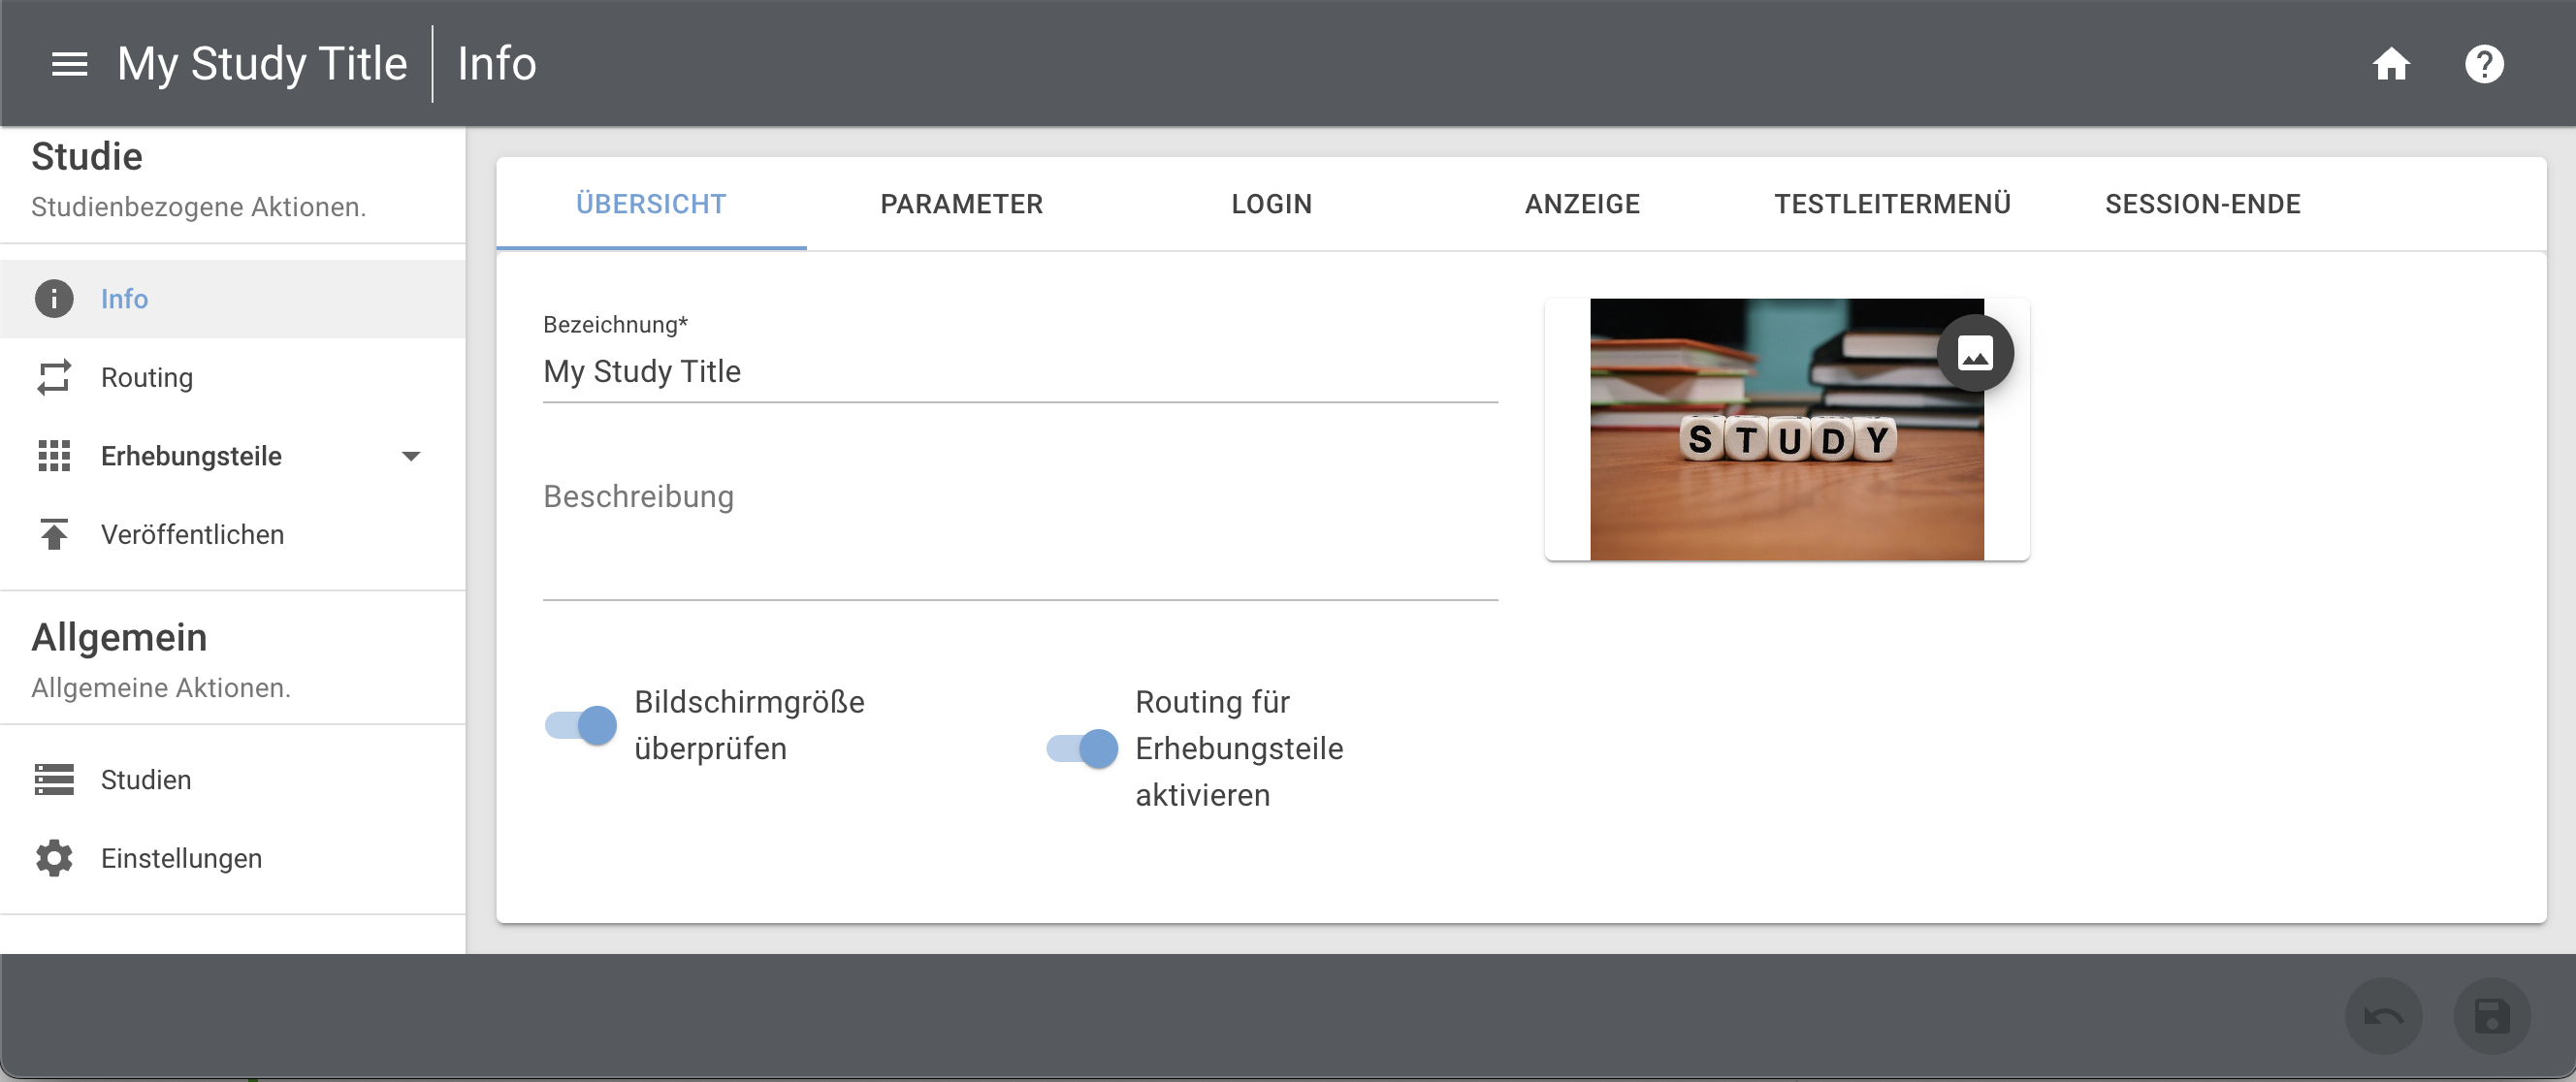
\includegraphics[width=1\textwidth,height=\textheight]{img/screenshot-studies-info.de-DEU.png}

Detaillierte Informationen zu der Grundkonfiguration einer Studie finden
sich hier in der eingebetteten Hilfe:

\begin{tcolorbox}[enhanced jigsaw, colbacktitle=quarto-callout-tip-color!10!white, coltitle=black, colframe=quarto-callout-tip-color-frame, leftrule=.75mm, breakable, opacitybacktitle=0.6, toprule=.15mm, title=\textcolor{quarto-callout-tip-color}{\faLightbulb}\hspace{0.5em}{Eingebettete Programmhilfe}, colback=white, titlerule=0mm, arc=.35mm, bottomtitle=1mm, toptitle=1mm, rightrule=.15mm, bottomrule=.15mm, left=2mm, opacityback=0]

\hypertarget{einstellungen-zur-studie-1}{%
\subsection{Einstellungen zur Studie}\label{einstellungen-zur-studie-1}}

\begin{itemize}
\item
  \textbf{Bezeichnung}: Wie soll die \emph{Studie} benannt werden?
  Achten Sie darauf, dass für die Bezeichnung nur Buchstaben (Groß- und
  Kleinschreibung), Ziffer und ein \texttt{\_} erlaubt sind.
\item
  \textbf{Beschreibung}: Um eine ausführliche Beschreibung der
  \emph{Studie} hinterlegen zu können, ist dieses optionle Feld
  vorgesehen. Hier können auch Sonderzeichen und Umlaute usw. eingegeben
  werden.
\item
  \textbf{Routing für Erhebungsteile aktivieren}: \emph{Studien}
  bestehen aus einem oder mehreren \emph{Erhebungsteilen}. Die
  \emph{Erhebungsteile} werden per Default als lineare Abfolge
  administriert. Wenn die Option \emph{Routing für Erhebungsteile
  aktivieren} ausgewählt ist, kann die Reihenfolge der
  \emph{Erhebungsteile} mit einem Blockly-basierten Routing definiert
  werden. Dadurch sind dynamische Abfolgen von \emph{Erhebungsteilen}
  möglich, wobei auch Aufrufparameter der Studie bspw. für die Zuordnung
  von unterschiedlichen Reihenfolgen genutzt werden können.
\item
  \textbf{Bildschirmgröße überprüfen}: In Erhebungen, bei denen die
  Bildschirmgröße nicht bekannt ist, kann mit dieser Option ein
  Größenvergleich von Objekten (EC-Karte, Banknote, Personalausweis) mit
  Darstellungen auf dem Bildschirm vorgenommen werden.
\end{itemize}

\begin{quote}
Die Geräteprüfung erfolgt mit folgendem Dialog:
\end{quote}

\begin{quote}
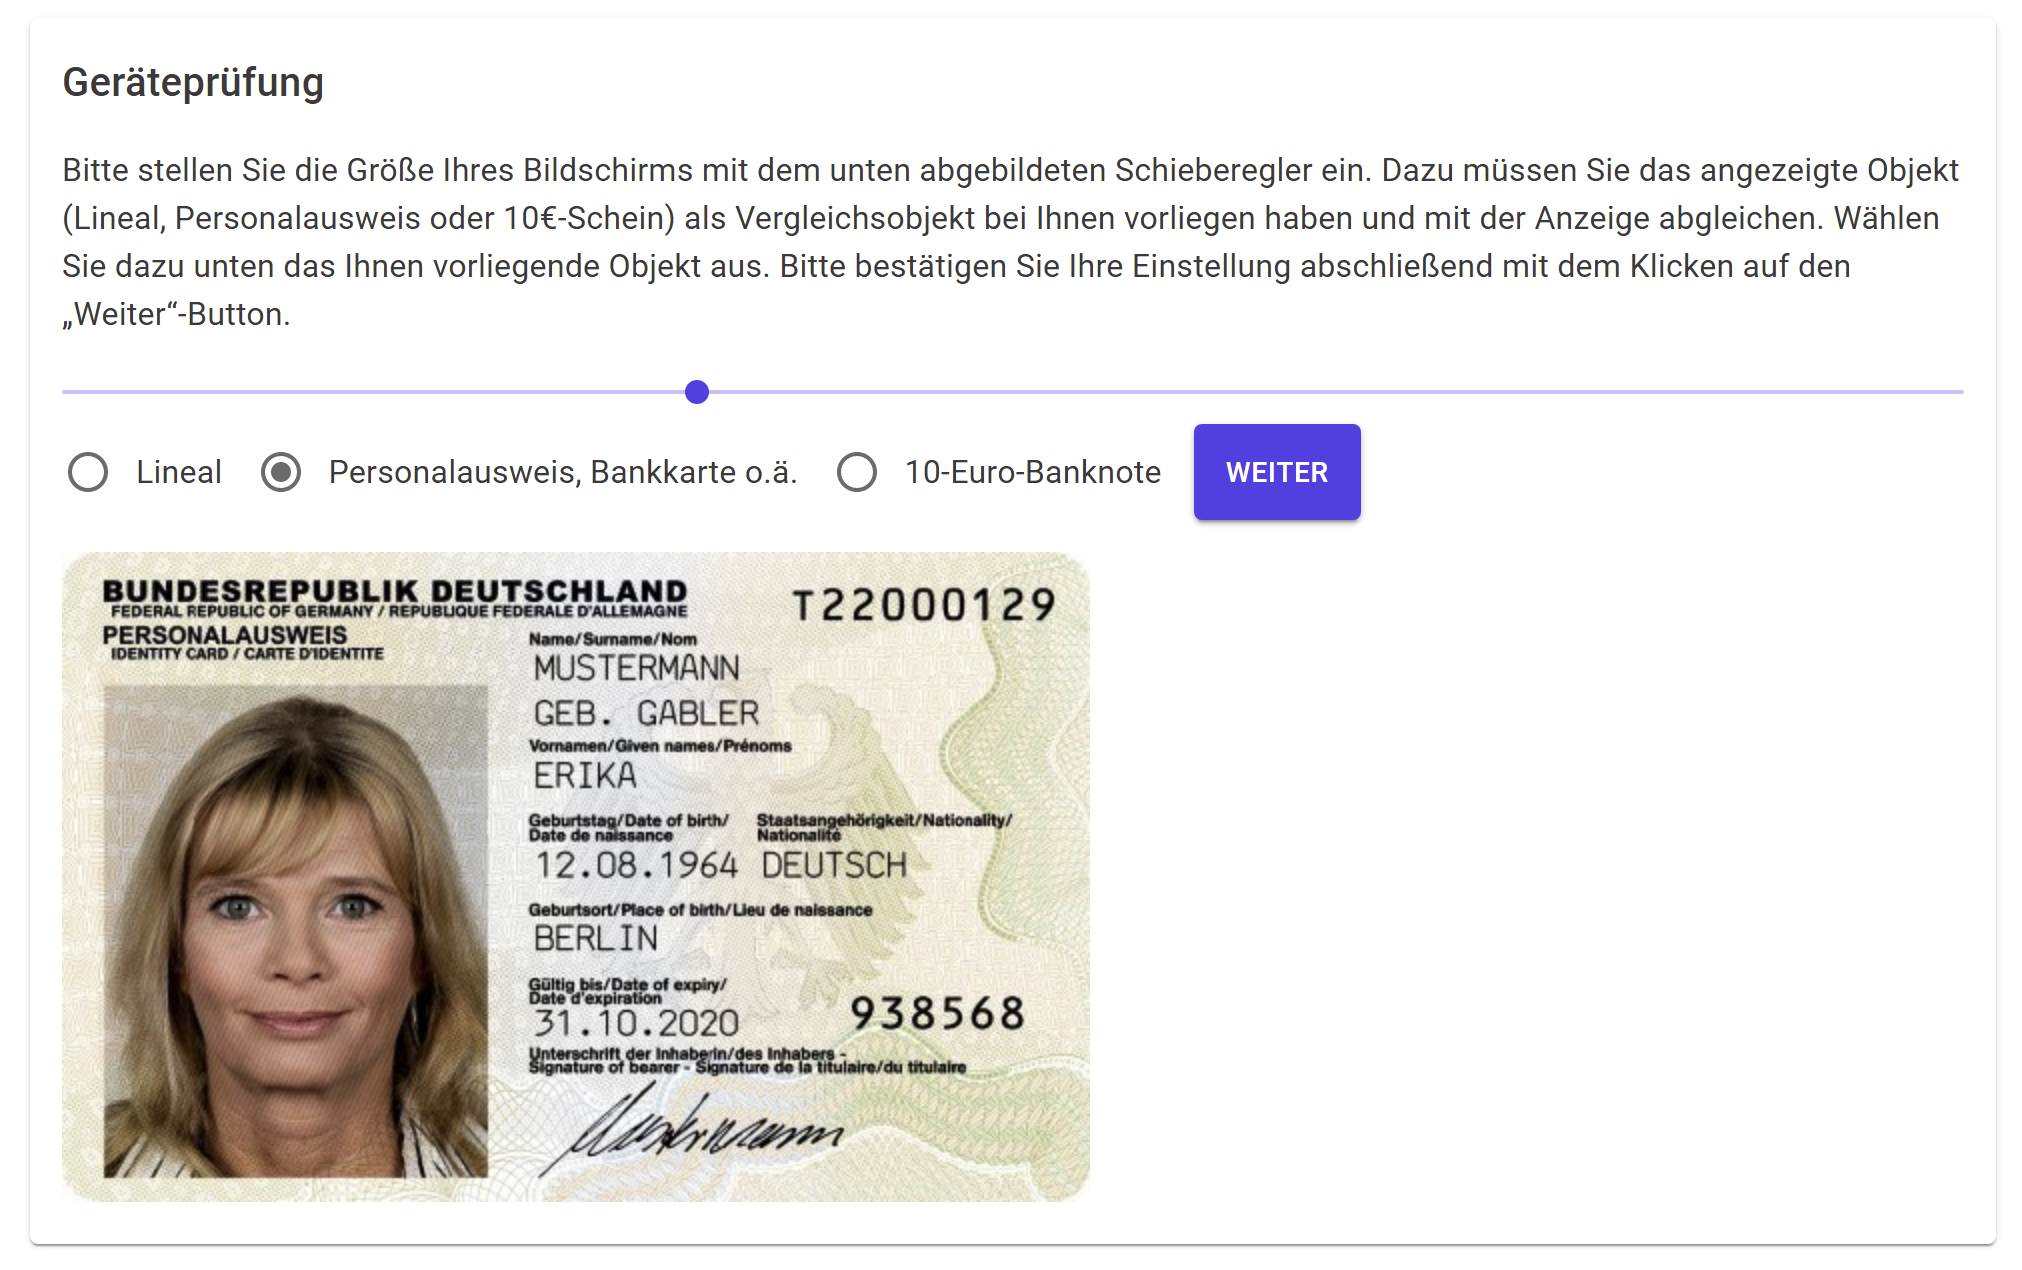
\includegraphics[width=4.16667in,height=\textheight]{img/screenshot-check-display-size-01-DEU.png}
\end{quote}

\begin{quote}
Wenn die Option \emph{Passende Bildschirmgröße erzwingen} (im Abschnitt
\emph{Anzeige}) nicht aktiviert ist, dann kann die Testbearbeitung
dennoch begonnen werden. Es wird, wenn die Auflösung zu klein ist,
folgender Dialog angezeigt:
\end{quote}

\begin{quote}
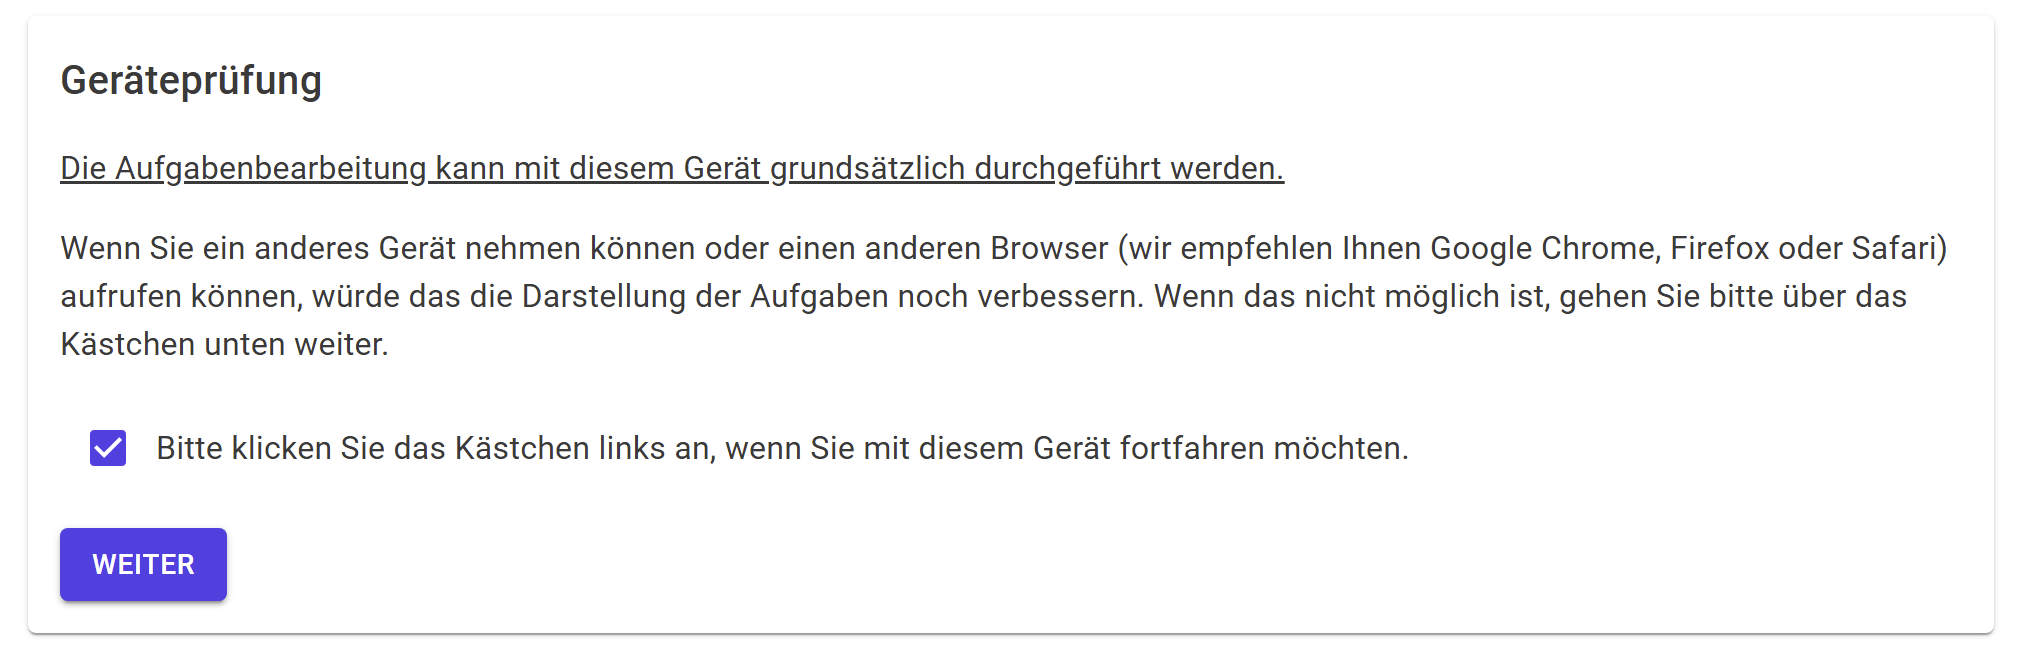
\includegraphics[width=4.16667in,height=\textheight]{img/screenshot-check-display-size-02-DEU.png}
\end{quote}

\begin{quote}
Hinweis: Diese Option ist zur Zeit nicht weiter konfigurierbar.
\end{quote}

Wenn geänderte Einstellungen erhalten bleiben sollen müssen die
Änderungen über das Disketten-Symbol gespeichert werden. Andernfalls
kann das Verwerfen-Symbol verwendet werden:

\begin{figure}[H]


\includegraphics[width=1.25in,height=\textheight]{img/screenshot-icons-undo-and-save-01.png} \hfill{}

\end{figure}

\end{tcolorbox}

\hypertarget{zugang-zu-studien-login-1}{%
\section{Zugang zu Studien (Login)}\label{zugang-zu-studien-login-1}}

Die \emph{IRTlib Software} unterstützt verschiedene Wege, wie sich
Personen (Testteilnehmer, Befragte, \ldots) für ein Assessment
Authentifizieren können. Die Konfiguratinen umfassen zwei Aspekte:

\begin{itemize}
\tightlist
\item
  \emph{Login-Modus}: Wird ein Zugang benötigt (Login, Login+Passwort,
  Passphrases/Token) oder nicht? Und wenn Zugangsdaten benötigt werden,
  was sind \emph{gültige Werge}?
\item
  \emph{Loginquelle}: Wie wird die Login-Information abgefragt (direkte
  Eingabe auf der Plattform, CBA ItemBuilder Item, \ldots.) oder
  übergeben (Login-Parameter oder Aufruf-Parameter)?
\end{itemize}

Detaillierte Informationen zu der Konfiguration der Anmeldung einer
\emph{Studie} finden sich hier in der eingebetteten Hilfe:

\begin{tcolorbox}[enhanced jigsaw, colbacktitle=quarto-callout-tip-color!10!white, coltitle=black, colframe=quarto-callout-tip-color-frame, leftrule=.75mm, breakable, opacitybacktitle=0.6, toprule=.15mm, title=\textcolor{quarto-callout-tip-color}{\faLightbulb}\hspace{0.5em}{Eingebettete Programmhilfe}, colback=white, titlerule=0mm, arc=.35mm, bottomtitle=1mm, toptitle=1mm, rightrule=.15mm, bottomrule=.15mm, left=2mm, opacityback=0]

\hypertarget{konfiguration-der-anmeldung-1}{%
\subsection{Konfiguration der
Anmeldung}\label{konfiguration-der-anmeldung-1}}

Im Abschnitt \emph{Login} kann konfiguriert werden, wie Testteilnehmer,
die ein Assessment starten (entweder durch Aufruf eines Links in einem
Browser der auf den Online-\emph{IRTlib-Player} verweist oder durch
Start des Offline-\emph{IRTlib-Players}), identifiziert oder
authentifiziert werden sollen.

\begin{itemize}
\item
  \textbf{Login-Modus}: Die \emph{IRTlib-Software} unterstützt
  verschiedene \emph{Login-Modi}.

  \begin{itemize}
  \item
    \emph{Zufälliger Inditifikator}: Wenn eine Sitzung zum ersten Mal
    gestartet wird, wird in diesem \emph{Login-Modus} ein Identifikator
    generiert. Diese zufällige, aber eindeutige Zeichenkette (eine
    sogenannte \emph{UUID}, d.h. ein \emph{Universally Unique
    Identifier}) wird als Personenidentifikator in allen Daten (d.h.
    Ergebnisdaten) und allen anderen gespeicherten Daten (z.B.
    Log-Daten/Trace-Daten, Snapshot-Daten, etc.) verwendet.
  \item
    \emph{Benutzername}: Wenn von den Testteilnehmern erwartet wird,
    dass sie sich durch eine eindeutige Zeichenfolge identifizieren
    (z.B. eine Zahl oder ein Text, der als Zugangskennung verwendet
    wird), kann eine \emph{Studie} mit dem \emph{Login-Modus}
    \emph{Benutzername} konfiguriert werden. Der Zugang zum Assessment
    ist dann nur möglich, wennd die als \emph{Benutzername} eingegebene
    Zeichenkette gültig ist. Die zugrundeliegende Idee ist, dass die
    Studienkonfiguration mit einer Liste gültiger Benutzernamen geladen
    wird und dass ein Testteilnehmer einen gültigen Benutzernamen
    eingeben muss, bevor er oder sie das Assessment starten kann. Nur
    authentifizierte Testteilnehmer können auf die als \emph{Studie}
    definierten Assessmentinhalte zugreifen und die Aufgaben bzw. Fragen
    beantworten.
  \item
    \emph{Benutzername und Passwort}: Wenn in einer \emph{Studie} nicht
    nur gültige Benutzernamen, sondern ein Passwort zur
    Authentifizierung der Testpersonen verwendet werden sollen,
    ermöglicht der \emph{Login-Modus} \emph{Benutzername und Passwort}
    eine Eingabe von Benutzernamen und Passwort. Analog zu
    \emph{Benutzername} müssen dann beide Informationen in der
    Studienkonfiguration hinterlegt sein.
  \item
    \emph{Zugriffstoken}: Wenn in der Studienkonfiguration die gültigen
    Benutzernamen nicht gespeichert werden sollen, kann die Option
    \emph{Zugriffstoken} verwendet werden. Jedes Token, das einem
    definierten Schema entspricht, wird dann akzeptiert und als
    Identifikator für die Testteilnehmer verwendet.
  \end{itemize}
\item
  \textbf{Speicher für Sessiondaten}: Bei Onlineauslieferungen kann nach
  einer Unterbrechung ein Assessment forgesetzt werden. Diese
  Funktionalität wird bspw. auch benötigt, wenn im Browser die Seite neu
  geladen wird (bspw. durch Erzwingen eines \emph{Reload}/F5, oder durch
  Schließen und erneutes Aufrufen der URL). Um sicherzustellen, dass
  Sitzungen, die von derselben Person (d.h. vom selben Browser) stammen,
  auch fortgesetzt werden können, kann die Software so konfiguriert
  werden, dass der Identifikator im Client gespeichert wird.
\item
  \textbf{Gültige Werte}: Die \emph{IRTlib-Software} bietet für die
  \emph{Login-Modu} \emph{Benutzername}, \emph{Benutzername + Passwort}
  und \emph{Zugriffstoken} folgende Mechanismen zur Validierung von
  Anmeldeinformationen:

  \begin{itemize}
  \item
    \emph{Liste}: Eine Liste gültiger Berechtigungen (Benutzername oder
    Benutzername und Passwort, je nach Konfiguration des
    \emph{Login-Modus}) kann als Teil der Studienkonfiguration definiert
    werden. Die Informationen können entweder im \emph{IRTlib-Editor}
    bearbeitet oder aus einer CSV-Datei importiert werden. Definierte
    Werte können auch als CSV-Datei exportiert werden.
  \item
    \emph{Code zur Prüfung}: Es kann eine \emph{Blockly}-Funktion
    angegeben werden, welche \emph{Wahr} zurückmeldet, wenn die
    übergebenen Anmeldedaten gültig sind (sonst \emph{Falsch}).
  \end{itemize}
\item
  \textbf{Gruppenlogin}: Je nach \emph{Login-Modus} dienen Benutzername
  oder Zugriffstoken als Personenidentifikator. Wenn die Option
  \emph{Gruppenanmeldung} aktiviert wird, dann werden diese übergebenen
  Anmeldedaten zur Authentifizierung verwendet, um den Testteilnehmer
  als Mitglied einer Gruppe zu identifizieren (d.~h. nur Testteilnehmer,
  die den Benutzernamen kennen, können sich als Teil der Gruppe
  authentifizieren). Innerhalb der Gruppe wird dann ein zusätzlicher
  Zufallsidentifikator generiert, um verschiedene Personen aus einer
  Gruppe zu unterscheiden.
\item
  \textbf{Loginquelle}: Die \emph{IRTlib-Software} unterstützt
  verschiedenen möglichen Optionen, wie für Anmeldeinformationen
  bereitgestellt werden können.

  \begin{itemize}
  \item
    \emph{Plattform}: Ein Anmeldedialog wird vom \emph{IRTlib-Player}
    (d.h. der Plattform) angezeigt. Die Überschrift zur Eingabe der
    Zugangsdaten, die Beschriftung der Eingabe für Benutzernamen und
    Passwort, die Beschriftung ddes Weiter-Buttons, dein Begrüßungs- und
    ein Instruktionstext sowie ein Fehlertextbei fehlgeschlagenen
    Login-Versuchen können konfiguriert werden.
  \item
    \emph{Parameter}: Gültige Anmeldedaten für Testteilnehmer können
    auch über die \emph{Befehlszeile} (d.h. Parameter beim Aufruf der
    Offline-Version des \emph{IRTlib Players}) oder über URL-Parameter
    (d.h. Parameter beim Aufruf der \emph{Studie} über einen Link auf
    eine Online-Version des \emph{IRTlib Players}) bereitgestellt
    werden. In diesem Fall wird kein Anmeldedialog oder Loginitem
    angezeigt.
  \item
    \emph{Item}: Alternativ zu einem Dialog des \emph{IRlLib-Players}
    kann auch ein \emph{CBA ItemBuilder}-Task konfiguriert werden, der
    als Login-Eingabemaske dient. Innerhalb des Items wird ein
    sogenannter \emph{ExternalPageFrame} verwendet, um zur Validierung
    einer Eingabe einen bestimmten JavaScript-Befehl an den
    \emph{IRlLib-Player} zu senden (ein Beispiel finden Sie
    \href{https://kroehne.github.io/CBAItemBuilderBook/items/10_00/IRTLibLoginExample.zip}{hier}).
  \end{itemize}
\end{itemize}

\begin{quote}
\begin{quote}
Das Login Item muss als \emph{CBA ItemBuilder} Projektdatei für die
konfigurierte Laufzeitumgebung (Runtime) verfügbar sein und der
Studienkonfiguration hinzugefügt werden. Um ein Login Item zur
Studienkonfiguration hinzuzufügen, kann der integrierte Importdialog
verwendet werden. Mehr Informationen zum Importieren von \emph{CBA
ItemBuilder}-Projekten findet sich in der Hilfe zum Abschnitt
\emph{Items} eines \emph{Erhebungsteils}.
\end{quote}
\end{quote}

\begin{itemize}
\item
  \textbf{Zusätzliche Parameter}: Neben der \emph{Authentifizierung} von
  Testteilnehmern können die Anmeldeinformationen in der
  \emph{IRTlib-Software} auch als zusätzlicher Parameter hinterlegt
  werden, die dann bspw. in der Ablaufsteuerung verwendet werden können.

  \begin{itemize}
  \item
    Parameter für Dateinamen: Der \texttt{RawDataPath} (d.h. der
    relative Pfad unter dem der Offline-\emph{IRTlib-Player} die
    Ergebnisdaten speichert) und der \texttt{MonitoringFile} (d.h. der
    Name der Datei in welcher der Offline-\emph{IRTlib-Player}
    Informationen fürs Studienmonitoring schreibt) können als Teil der
    Anmeldedaten konfiguriert werden.
  \item
    \emph{Blockly}-Variablen: Zusätzliche Parameter können auch als
    sogenannte \emph{Preload}-Variablen mit den Anmeldeinformationen
    hinterlegt werde.
  \end{itemize}
\end{itemize}

\hypertarget{tbl-letters}{}
\begin{longtable}[]{@{}
  >{\centering\arraybackslash}p{(\columnwidth - 10\tabcolsep) * \real{0.1667}}
  >{\centering\arraybackslash}p{(\columnwidth - 10\tabcolsep) * \real{0.1667}}
  >{\centering\arraybackslash}p{(\columnwidth - 10\tabcolsep) * \real{0.1667}}
  >{\centering\arraybackslash}p{(\columnwidth - 10\tabcolsep) * \real{0.1667}}
  >{\centering\arraybackslash}p{(\columnwidth - 10\tabcolsep) * \real{0.1667}}
  >{\centering\arraybackslash}p{(\columnwidth - 10\tabcolsep) * \real{0.1667}}@{}}
\caption{\label{tbl-letters}Zusammenfassung der Optionen, die als
\emph{Konfiguration der Anmeldung} kombiniert werden
können}\tabularnewline
\toprule\noalign{}
\begin{minipage}[b]{\linewidth}\centering
Login Modus
\end{minipage} & \begin{minipage}[b]{\linewidth}\centering
Speicher für Sessiondaten
\end{minipage} & \begin{minipage}[b]{\linewidth}\centering
Gruppenlogin
\end{minipage} & \begin{minipage}[b]{\linewidth}\centering
Gültige Werte
\end{minipage} & \begin{minipage}[b]{\linewidth}\centering
Loginquelle
\end{minipage} & \begin{minipage}[b]{\linewidth}\centering
Zusätzliche Parameter
\end{minipage} \\
\midrule\noalign{}
\endfirsthead
\toprule\noalign{}
\begin{minipage}[b]{\linewidth}\centering
Login Modus
\end{minipage} & \begin{minipage}[b]{\linewidth}\centering
Speicher für Sessiondaten
\end{minipage} & \begin{minipage}[b]{\linewidth}\centering
Gruppenlogin
\end{minipage} & \begin{minipage}[b]{\linewidth}\centering
Gültige Werte
\end{minipage} & \begin{minipage}[b]{\linewidth}\centering
Loginquelle
\end{minipage} & \begin{minipage}[b]{\linewidth}\centering
Zusätzliche Parameter
\end{minipage} \\
\midrule\noalign{}
\endhead
\bottomrule\noalign{}
\endlastfoot
Zufälliger Inditifikator & ja & nein & nein & keine & nein \\
Benutzername & ja & ja & Liste oder Code & Plattform, Item + Parameter &
Werte oder Parameter \\
Benutzername und Passwort & ja & ja & Liste oder Code & Plattform, Item
+ Parameter & Werte oder Parameter \\
Zugriffstoken & ja & ja & Schema oder Code & Plattform, Item + Parameter
& Parameter \\
\end{longtable}

\end{tcolorbox}

\hypertarget{anzeige-von-assessment-inhalten-1}{%
\section{Anzeige von
Assessment-Inhalten}\label{anzeige-von-assessment-inhalten-1}}

\emph{Studien} können festlegen, wie der \emph{CBA ItemBuilder}-Inhalt
dargestellt werden soll. Die Einstellungen im Aschnitt \emph{Anzeige}
können sich auf die Skalierung und die Ausrichtung der Inhalte sowie auf
das Verhalten der \emph{IRTlib Player}-Anwendung beziehen.

Detaillierte Informationen zu der Konfiguration der \emph{Anzeige} einer
\emph{Studie} finden sich hier in der eingebetteten Hilfe:

\begin{tcolorbox}[enhanced jigsaw, colbacktitle=quarto-callout-tip-color!10!white, coltitle=black, colframe=quarto-callout-tip-color-frame, leftrule=.75mm, breakable, opacitybacktitle=0.6, toprule=.15mm, title=\textcolor{quarto-callout-tip-color}{\faLightbulb}\hspace{0.5em}{Eingebettete Programmhilfe}, colback=white, titlerule=0mm, arc=.35mm, bottomtitle=1mm, toptitle=1mm, rightrule=.15mm, bottomrule=.15mm, left=2mm, opacityback=0]

\hypertarget{anzeigeeinstellungen-1}{%
\subsection{Anzeigeeinstellungen}\label{anzeigeeinstellungen-1}}

Für die Konfiguration der Anzeige stehen ausgewählte Optionen zur
Verfügung, die sich auf die Darstellung der Assessmentinhalte und die
Verwendung von \emph{CBA ItemBuilder}-Inhalten beziehen, welche mit
einem festgelegten Seitenverhältnis (Breite und Höhe) erstellt werden.

\hypertarget{fenstermodus-1}{%
\subsubsection{Fenstermodus}\label{fenstermodus-1}}

In der Auswahl \textbf{Fenstermodus} kann konfiguriert werden, ob ein
zusätzliches Fenster im \emph{IRTlib Player} angezeigt wird. Die
Konfiguration wird je nach Umgebung unterschiedlich umgesetzt:

\begin{itemize}
\tightlist
\item
  \emph{Window}: In diesem \emph{Fenstermodus} wird im
  Offline-\emph{IRTlib Player} ein reguläres Programmfenster verwendet,
  im Online-\emph{IRTlib Player} wird der Assessmentinhalt im normalen
  Browserbereich angezeigt, und die Adressleiste und die
  Navigationsschaltflächen des Browsers sind in diesem Modus sichtbar.
\end{itemize}

\begin{quote}
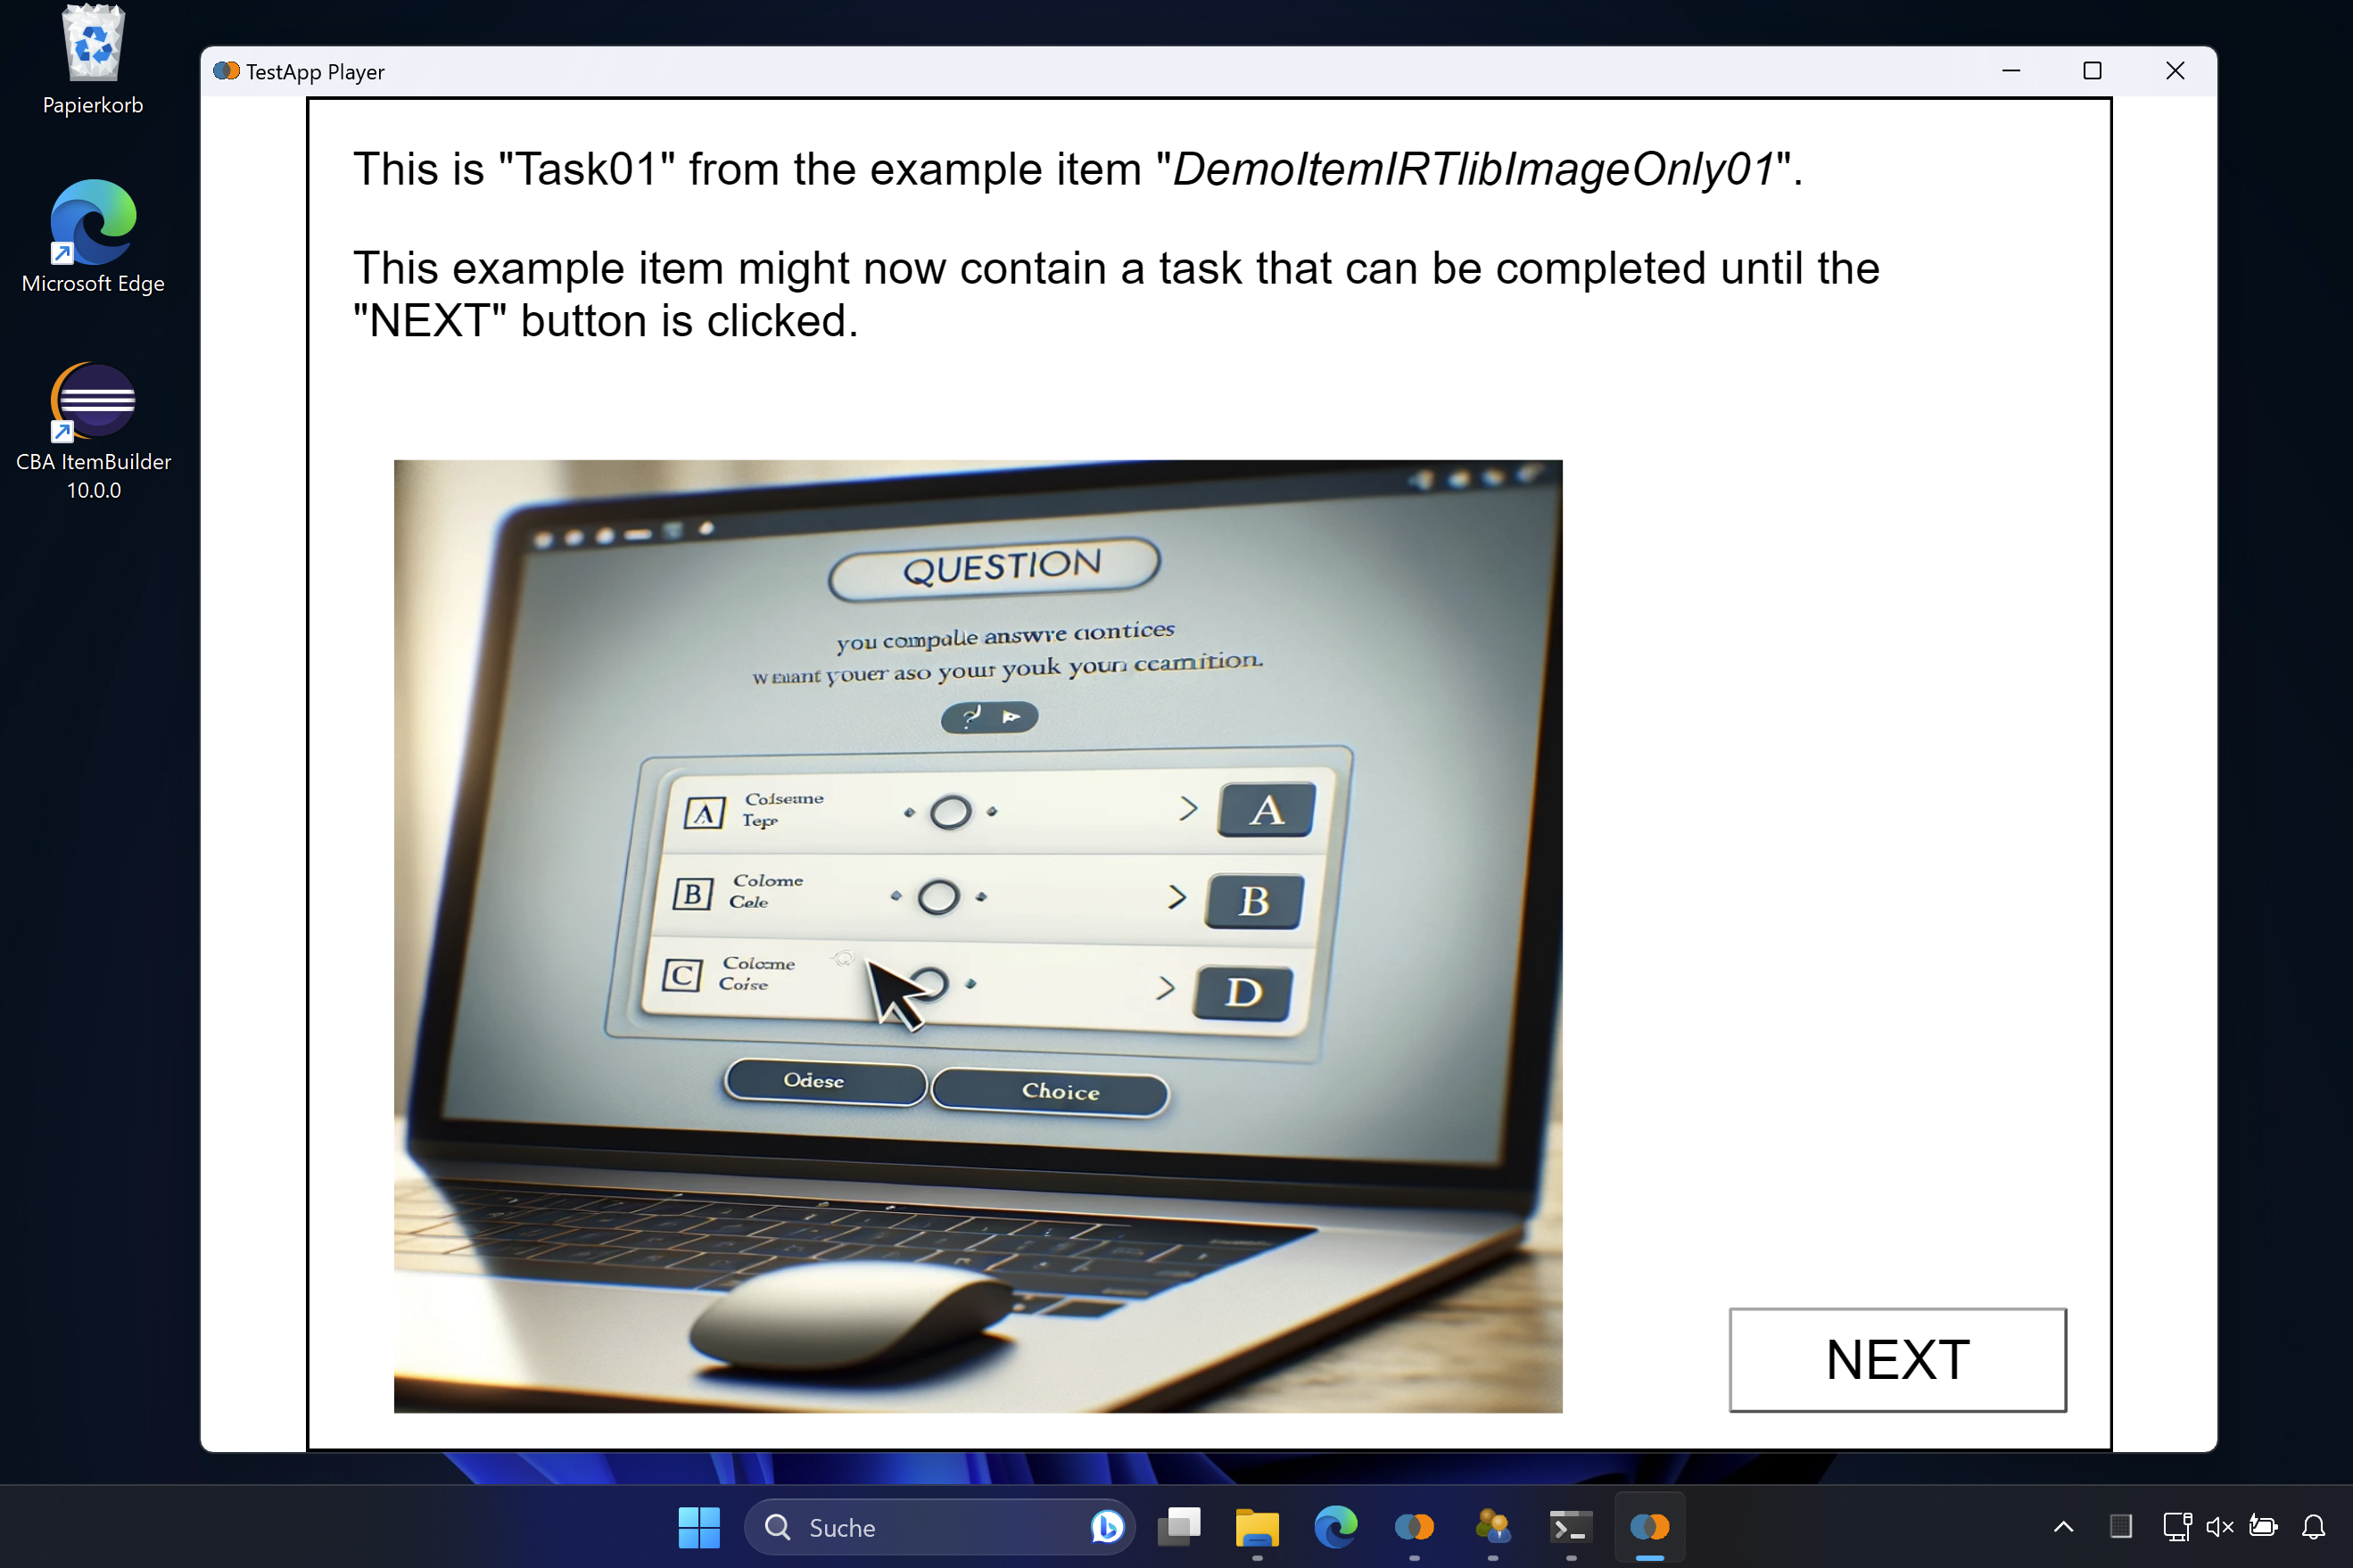
\includegraphics[width=0.8\textwidth,height=\textheight]{img/screenshot-window-mode-example-offline-player-01.png}
\end{quote}

\begin{itemize}
\tightlist
\item
  \emph{Vollbild}: Der Offline-\emph{IRTlib Player} startet direkt im
  Vollbildmodus, wenn diese Option konfiguriert ist. Damit verbunden ist
  auch ein \emph{Kiosk-Modus}, d.h. der Zugriff auf andere Programme und
  das (versehentliche) Beenden des Programms ist nur über den \emph{Task
  Manager} möglich. Soll die Möglichkeit zum Beenden der Testung bspw.
  für einen Testleiter möglich sein, muss ein \emph{Testleitermenü}
  konfiguriert sein.
\end{itemize}

\begin{quote}
Der Online-\emph{IRlLib Player} kann Assessmentinhalte auch im
Vollbildmodus an, wenn diese Option gewählt ist. Wird der Vollbildmodus
im Browser verlassen, wird dann der Assessmentinhalt ausgeblendet. Da
automatisiert nicht in einem Browser in den Vollbildmodus gewechselt
werden kann, sieht die Zielperson zunächst folgende Nachricht der
Plattform:
\end{quote}

\begin{quote}
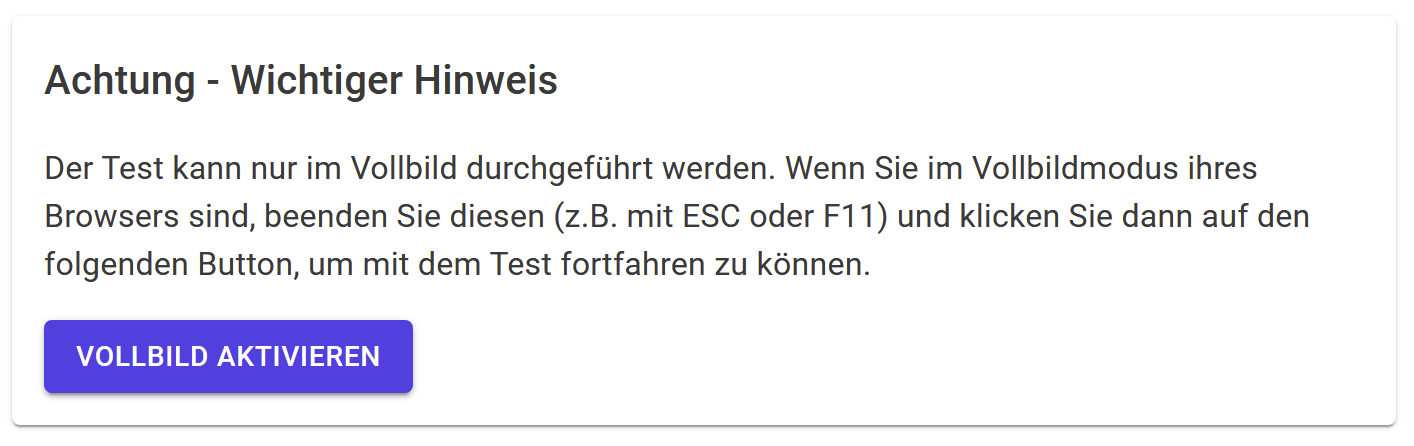
\includegraphics[width=0.8\textwidth,height=\textheight]{img/screenshot-irtlib-player-message-fullscreen-not-started-DEU.png}
\end{quote}

\begin{quote}
Durch klick auf den Button \emph{Vollbild Aktivieren} wird der
Vollbildmodus gestartet und der Assessmentinhalt dann ohne Fensterrahmen
und Navigationsflächen des Browsers dargestellt. Für kurze Zeit wird
dann von den Browser typischerweise ein Hinweis eingeblendet dass mit
\texttt{Esc}der Vollbildmodus wieder beendet werden kann.
\end{quote}

\begin{quote}
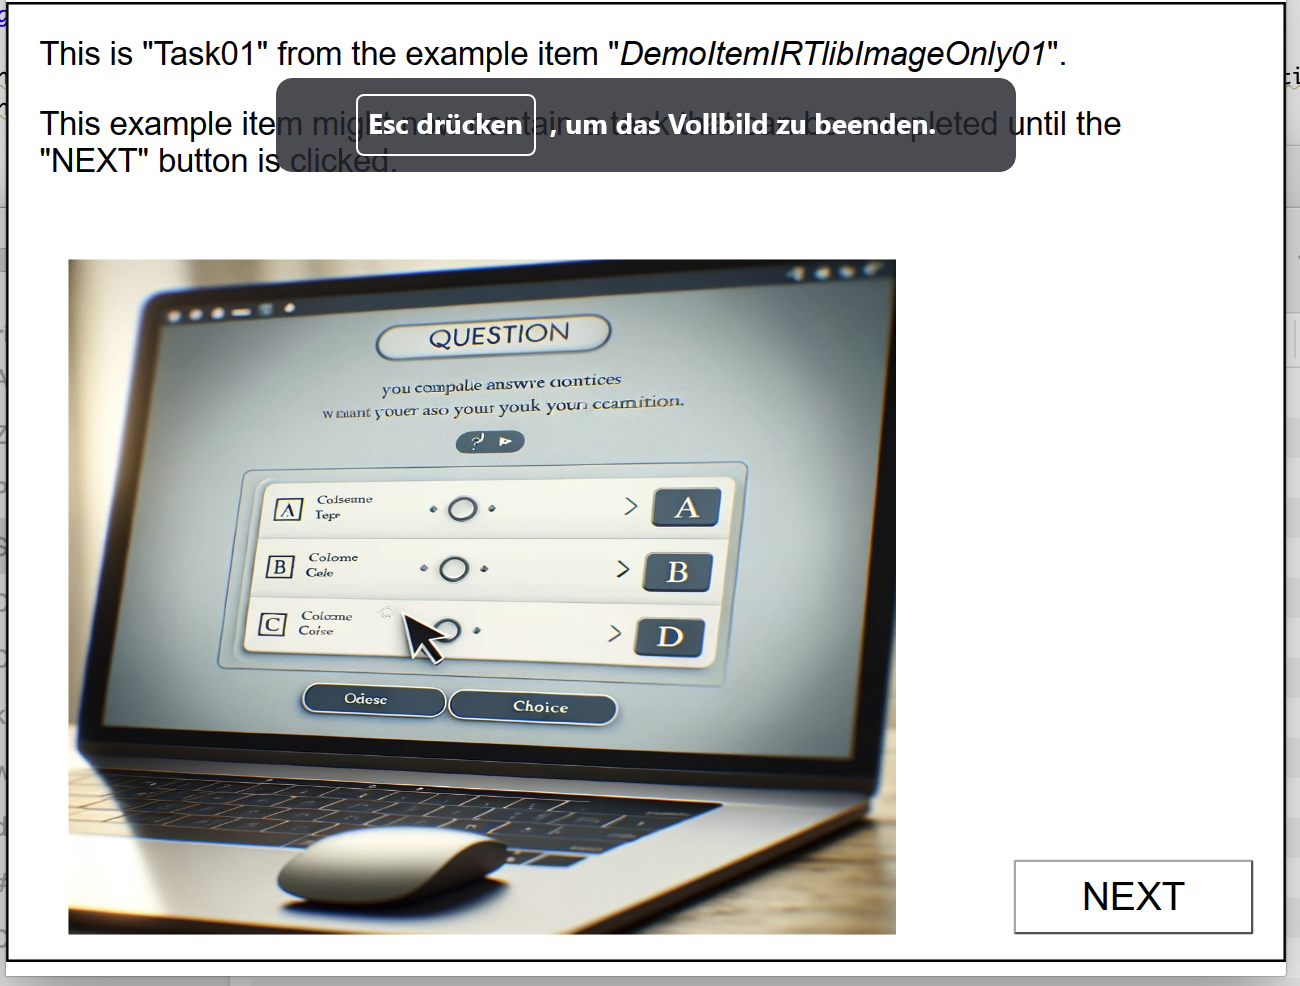
\includegraphics[width=0.8\textwidth,height=\textheight]{img/screenshot-irtlib-player-message-fullscreen-notification-DEU.png}
\end{quote}

\begin{quote}
Beachten Sie, dass diese Funktion nur in Browsern zur Verfügung steht,
die den Vollbildmodus unterstützen (insbesondere auf älteren mobilen
Geräten wird der Vollbildmodus nicht vollständig unterstützt; siehe für
Details z.B. auf
\href{https://caniuse.com/?search=fullscreen}{caniuse.com}).
\end{quote}

\begin{itemize}
\tightlist
\item
  \emph{Vollbild, wenn unterstützt}: In diesem Modus wird das Assessment
  im Online-\emph{IRTlib Player} nur dann im im Vollbildmodus angezeigt,
  wenn der Browser den Vollbildmodus unterstützt. Der Inhalt des
  computerbasierten Assessments wird jedoch im Fenstermodus angezeigt,
  wenn eine Studie online bereitgestellt wird und ein Browser verwendet
  wird, der den Vollbildmodus nicht unterstützt. Für den \emph{IRlLib
  Player} offline ist diese Konfiguration identisch mit \emph{Vollbild}.
\end{itemize}

\begin{quote}
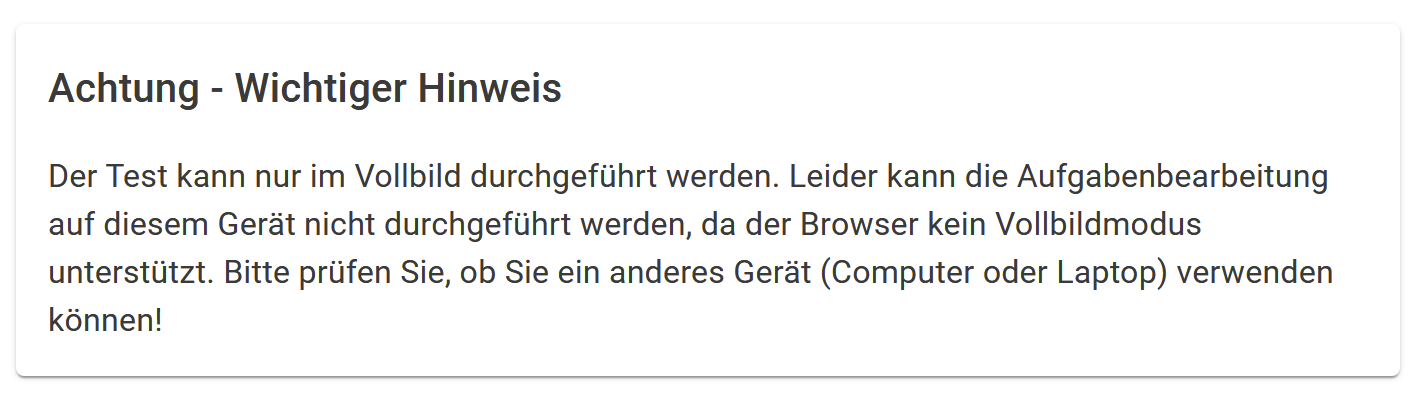
\includegraphics[width=0.8\textwidth,height=\textheight]{img/screenshot-irtlib-player-message-fullscreen-not-supported-DEU.png}
\end{quote}

\begin{itemize}
\tightlist
\item
  \emph{Debug}: Dieser Modus ermöglicht während der Testausführung den
  Zugriff auf die Entwicklerwerkzeuge des Browsers, die für die
  Fehlersuche von Softwareentwicklern vorgesehen sind.
\end{itemize}

\begin{quote}
Wennd der Offline-\emph{IRTlib Player} mit einer Studie gestartet wird,
welche als \emph{Festermodus} den Eintrag \emph{Debug} konfiguriert hat,
dann lassen sich über die rechte Maustaste während der
Aufgabenpräsentation die sogenannten Entwickertools (\emph{DevTools})
abrufen.
\end{quote}

\begin{quote}
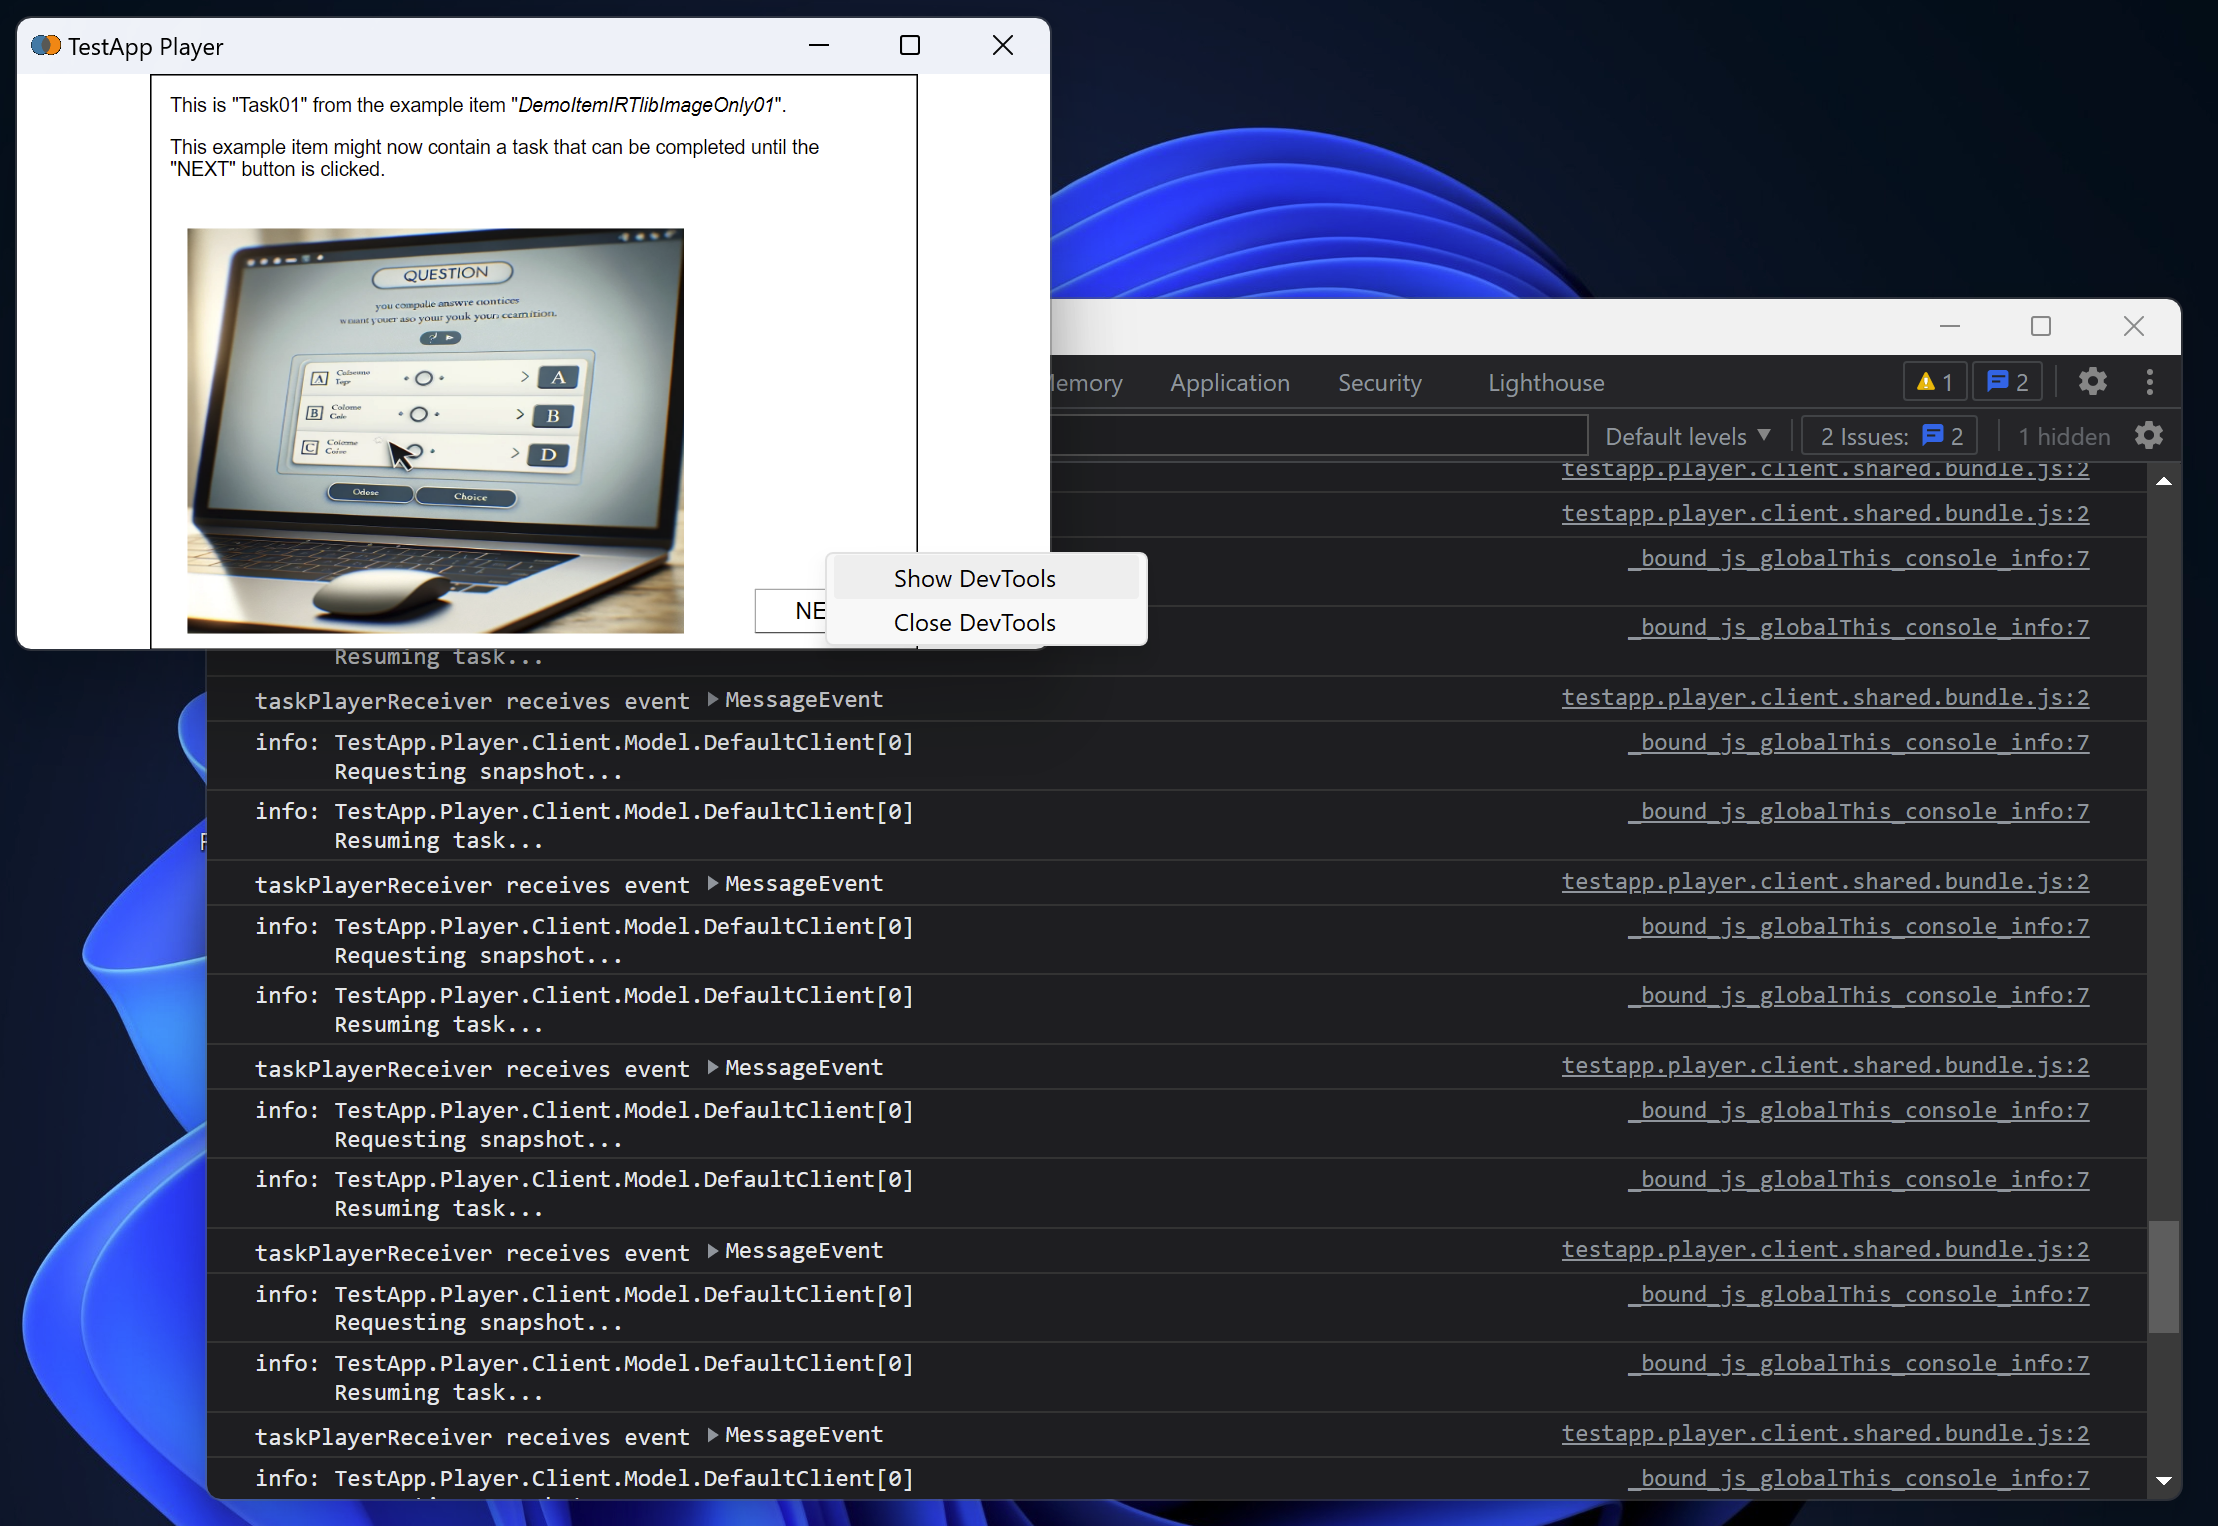
\includegraphics[width=0.8\textwidth,height=\textheight]{img/screenshot-debug-view-dev-tools-example-01.png}
\end{quote}

\hypertarget{skalierung-und-ausrichtung-1}{%
\subsection{Skalierung und
Ausrichtung}\label{skalierung-und-ausrichtung-1}}

Assessmentinhalte, die mit dem \emph{CBA ItemBuilder} erstellt werden,
werden für eine konkrete Größe in Pixeln (Breite mal Höhe) erstellt. Für
die Darstellung auf Geräten mit unterschiedlichen Bildschirmgröße und
Bildschirmauflösungen können die Inhalte dann skaliert werden. Im
\emph{CBA ItemBuilder} stehen deshalb in der \emph{Preview} die Optione
unter \emph{Scaling Options} zur Verfügung:

\begin{quote}
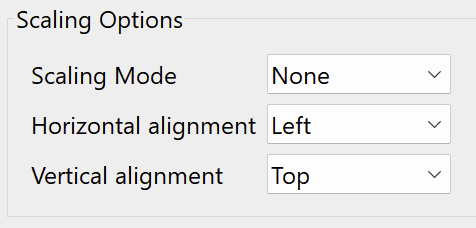
\includegraphics[width=2.08333in,height=\textheight]{img/screenshot-cba-itembuilder-preview-scaling-mode-01.png}
\end{quote}

Im \emph{IRTlib Editor} können analoge Einstellung vorgenommen werden.

\begin{itemize}
\item
  \textbf{Skalierung}: Einstellung wie Inhalte angepasst werden sollen,
  wenn verfügbarer Platz und Größe der Items abweichen (\emph{Scaling
  Mode}).

  \begin{itemize}
  \tightlist
  \item
    \emph{keine}: Die Inhalte werden ohne Anpassung an die verfügbare
    Fenster- bzw. Bildschirmgröße angezeigt (entspricht \texttt{None}).
  \item
    \emph{hochskalieren}: Inhalte werden vergrößert, damit der
    verfügbare Platz ausgenutzt wird (entspricht \texttt{Up}).
  \item
    \emph{runterskalieren}: Inhalte werden verkleinert, damit sie auf
    den Bildschirm/ins Fenster passen (entspricht \texttt{Down}).
  \item
    \emph{Fenstergröße}: Inhalte werden vergrößert und verkleinert
    (entspricht \texttt{Both}).
  \end{itemize}
\item
  \textbf{Horizontale Ausrichtung}: Die Optionen \emph{zentriert} /
  \emph{links} / \emph{rechts} werden genutzt um Iteminhalte horizontal
  auszurichten, wenn die Breite von Fenster oder Bildschirm größer ist
  als die Breite des Inhalts.
\item
  \textbf{Vertikale Ausrichtung}: Die Optionen \emph{zentriert} /
  \emph{oben} / \emph{unten} werden genutzt um Iteminhalte vertikal
  auszurichten, wenn die Höhe von Fenster oder Bildschirm größer ist als
  die Höhe des Inhalts.
\end{itemize}

\hypertarget{weitere-einstellungen-1}{%
\subsubsection{Weitere Einstellungen}\label{weitere-einstellungen-1}}

\begin{itemize}
\tightlist
\item
  \textbf{Passende Bildschirmgröße erzwingen}: Wenn bei
  \emph{Skalierung} nicht \emph{runterskalieren} oder
  \emph{Fenstergröße} ausgewählt ist, kann über diese Option erzwungen
  werden, dass man nur dann mit der Aufgabenbearbeitung starten kann,
  wenn die verfügbare Größe des Fensters bzw. Bildschirms größer ist als
  die benötigte Breite/Höhe der Items. Andernfalls wird folgende
  Nachricht angezeigt:
\end{itemize}

\begin{quote}
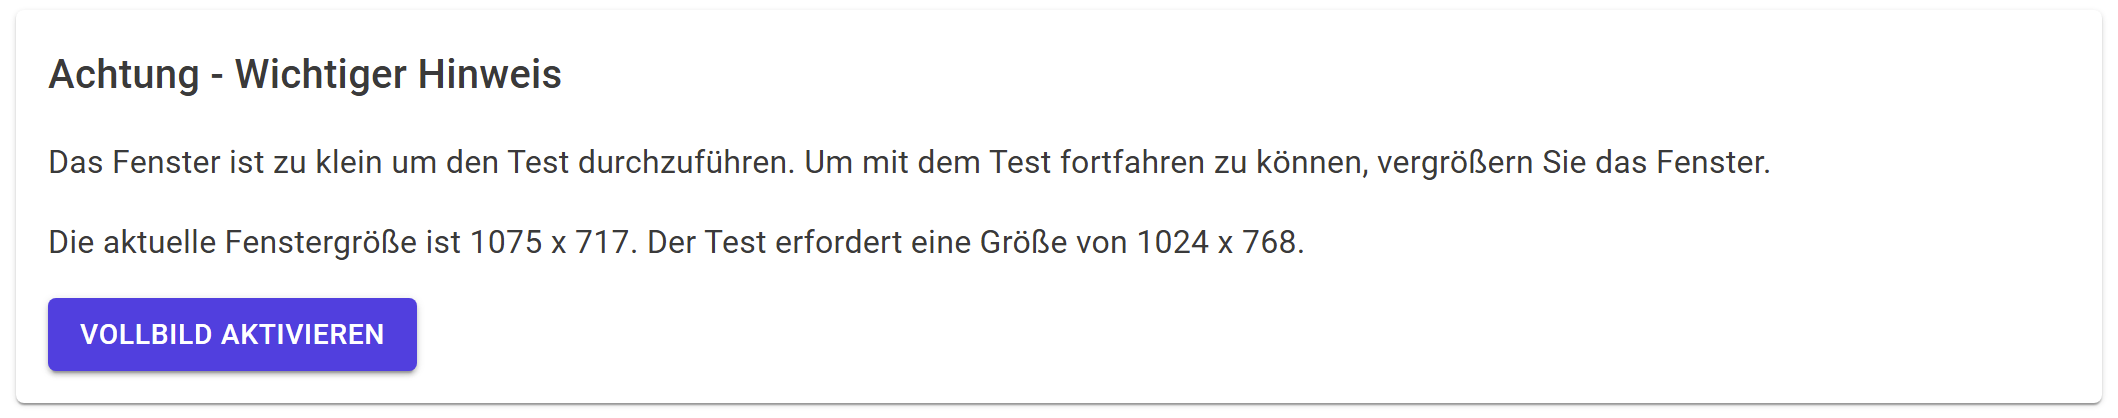
\includegraphics[width=0.8\textwidth,height=\textheight]{img/screenshot-irtlib-player-message-resolution-too-low-DEU.png}
\end{quote}

Hinweis: Die Einstellungen zur Anzeige beziehen sich auf alle
\emph{Erhebungsteile} innerhalb einer \emph{Studie}. Werden in einem
\emph{IRTlib-Player} mehrere Studien konfiguriert, müssen die
Einstellungen zueinander passen, d.h. es ist nicht mögliche mit einer
Instanz eines \emph{IRTlib-Players} gleichzeitig eine Studie im
\emph{Fenstermodus: Fenster} oder im \emph{Fenstermodus: Vollbild} zu
adminsitrieren.

Wenn geänderte Einstellungen erhalten bleiben sollen müssen die
Änderungen über das Disketten-Symbol gespeichert werden. Andernfalls
kann das Verwerfen-Symbol verwendet werden:

\begin{figure}[H]


\includegraphics[width=1.25in,height=\textheight]{img/screenshot-icons-undo-and-save-01.png} \hfill{}

\end{figure}

\end{tcolorbox}

\hypertarget{menuxfc-fuxfcr-testadministratoren-1}{%
\section{Menü für
Testadministratoren}\label{menuxfc-fuxfcr-testadministratoren-1}}

Wenn die Durchführung von Assessments begleitet durch Testleiter oder
Interviewer erfolgt, können Funktionen passwortgeschützt für Testleiter
definiert werden.

\begin{tcolorbox}[enhanced jigsaw, colbacktitle=quarto-callout-warning-color!10!white, coltitle=black, colframe=quarto-callout-warning-color-frame, leftrule=.75mm, breakable, opacitybacktitle=0.6, toprule=.15mm, title=\textcolor{quarto-callout-warning-color}{\faExclamationTriangle}\hspace{0.5em}{Warnung}, colback=white, titlerule=0mm, arc=.35mm, bottomtitle=1mm, toptitle=1mm, rightrule=.15mm, bottomrule=.15mm, left=2mm, opacityback=0]

Auch wenn Sie die Funktionalität eines Testadministratormenüs für die
Durchführung Ihrer Datenerfassung nicht benötigen, sollten Sie dennoch
ein Testadministratormenü definieren, wenn Sie planen, mit dem
\emph{IRTlib Player} Daten offline zu erfassen. Nur so können Sie
sicherstellen, dass Sie die Anwendung im Falle unvorhergesehener
Ereignisse ohne den Task-Manager (und ohne möglichen Datenverlust)
beenden können.

\end{tcolorbox}

Detaillierte Informationen zu der Konfiguration des
\emph{Testleitermenüs} finden sich hier in der eingebetteten Hilfe:

\begin{tcolorbox}[enhanced jigsaw, colbacktitle=quarto-callout-tip-color!10!white, coltitle=black, colframe=quarto-callout-tip-color-frame, leftrule=.75mm, breakable, opacitybacktitle=0.6, toprule=.15mm, title=\textcolor{quarto-callout-tip-color}{\faLightbulb}\hspace{0.5em}{Eingebettete Programmhilfe}, colback=white, titlerule=0mm, arc=.35mm, bottomtitle=1mm, toptitle=1mm, rightrule=.15mm, bottomrule=.15mm, left=2mm, opacityback=0]

\hypertarget{konzept-eines-testleitermenuxfcs-menuxfc-fuxfcr-testadministratoren-1}{%
\subsection{Konzept eines Testleitermenüs (Menü für
Testadministratoren)}\label{konzept-eines-testleitermenuxfcs-menuxfc-fuxfcr-testadministratoren-1}}

Die Konfiguration des Menü für Testadministratoren erfolgt in zwei
Schritten. Zunächst muss eine Tastenkombination definiert werden, mit
der das Testmanager-Menü aufgerufen werden kann. Wird diese
Tastenkombination während der Testbearbeitung gedrückt, erscheint ein
Fenster zur Passworteingabe. Testadministratoren geben das (nur) ihnen
bekannte Passwort ein und erhalten so Zugriff auf ausgewählte
Funktionen. Zu diesem Zweck müssen in einem zweiten Schritt eine oder
mehrere Rollen im \emph{IRTlib Editor} definiert werden.

\hypertarget{zugriff-fuxfcr-testleitung-1}{%
\subsubsection{Zugriff für
Testleitung}\label{zugriff-fuxfcr-testleitung-1}}

Zunächst muss eine Tastenkombination definiert werden.

\begin{itemize}
\item
  \textbf{Taste}: Die Konfiguration der Tastenkombination für das
  Testleitermenü erfordert zunächst die Definition einer Taste. Um eine
  Taste festzulegen klickt man in das Feld und drückt die Taste, welche
  für das Testleitermenü verwendet werden soll.
\item
  \textbf{Modifikatoren} (Alt, Strg und Shift): Für eine Taste kann dann
  zusätzlich festgelegt werden, ob eine oder mehrere Modifkatoren
  gedrück werden müssen damit das Testleitermenü geöffnet wird.
\end{itemize}

Beispiel:

\begin{itemize}
\tightlist
\item
  Die folgende Konfiguration definiert die Tastenkombination
  \texttt{Strg} + \texttt{Shift}+ \texttt{X}:
\end{itemize}

\begin{quote}
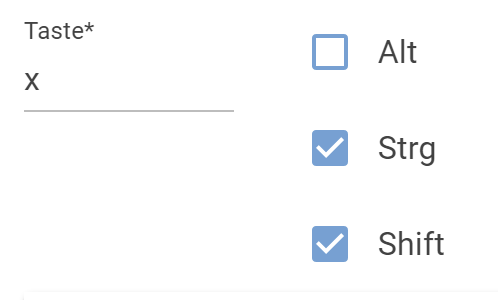
\includegraphics[width=2.08333in,height=\textheight]{img/screenshot-test-adminstrator-strg-shift-x-example-01.png}
\end{quote}

Die definierte Tastenkombination öffnet nur die Option zur Eingabe eines
Passowrt für Testleiter während der Testbearbeitung im \emph{IRTlib
Player}. Um die Funktion zu nutzen ist ein Passwot notwendig, welches
zusammen mit einer Rolle im zweiten Schritt definiert wird.

\hypertarget{rollen-1}{%
\subsubsection{Rollen}\label{rollen-1}}

Nach dem Aufruf der definierten Tastenkombination wird während der
Testbearbeitung die Aufforderung zur Eingabe eines Passworts angezeigt:

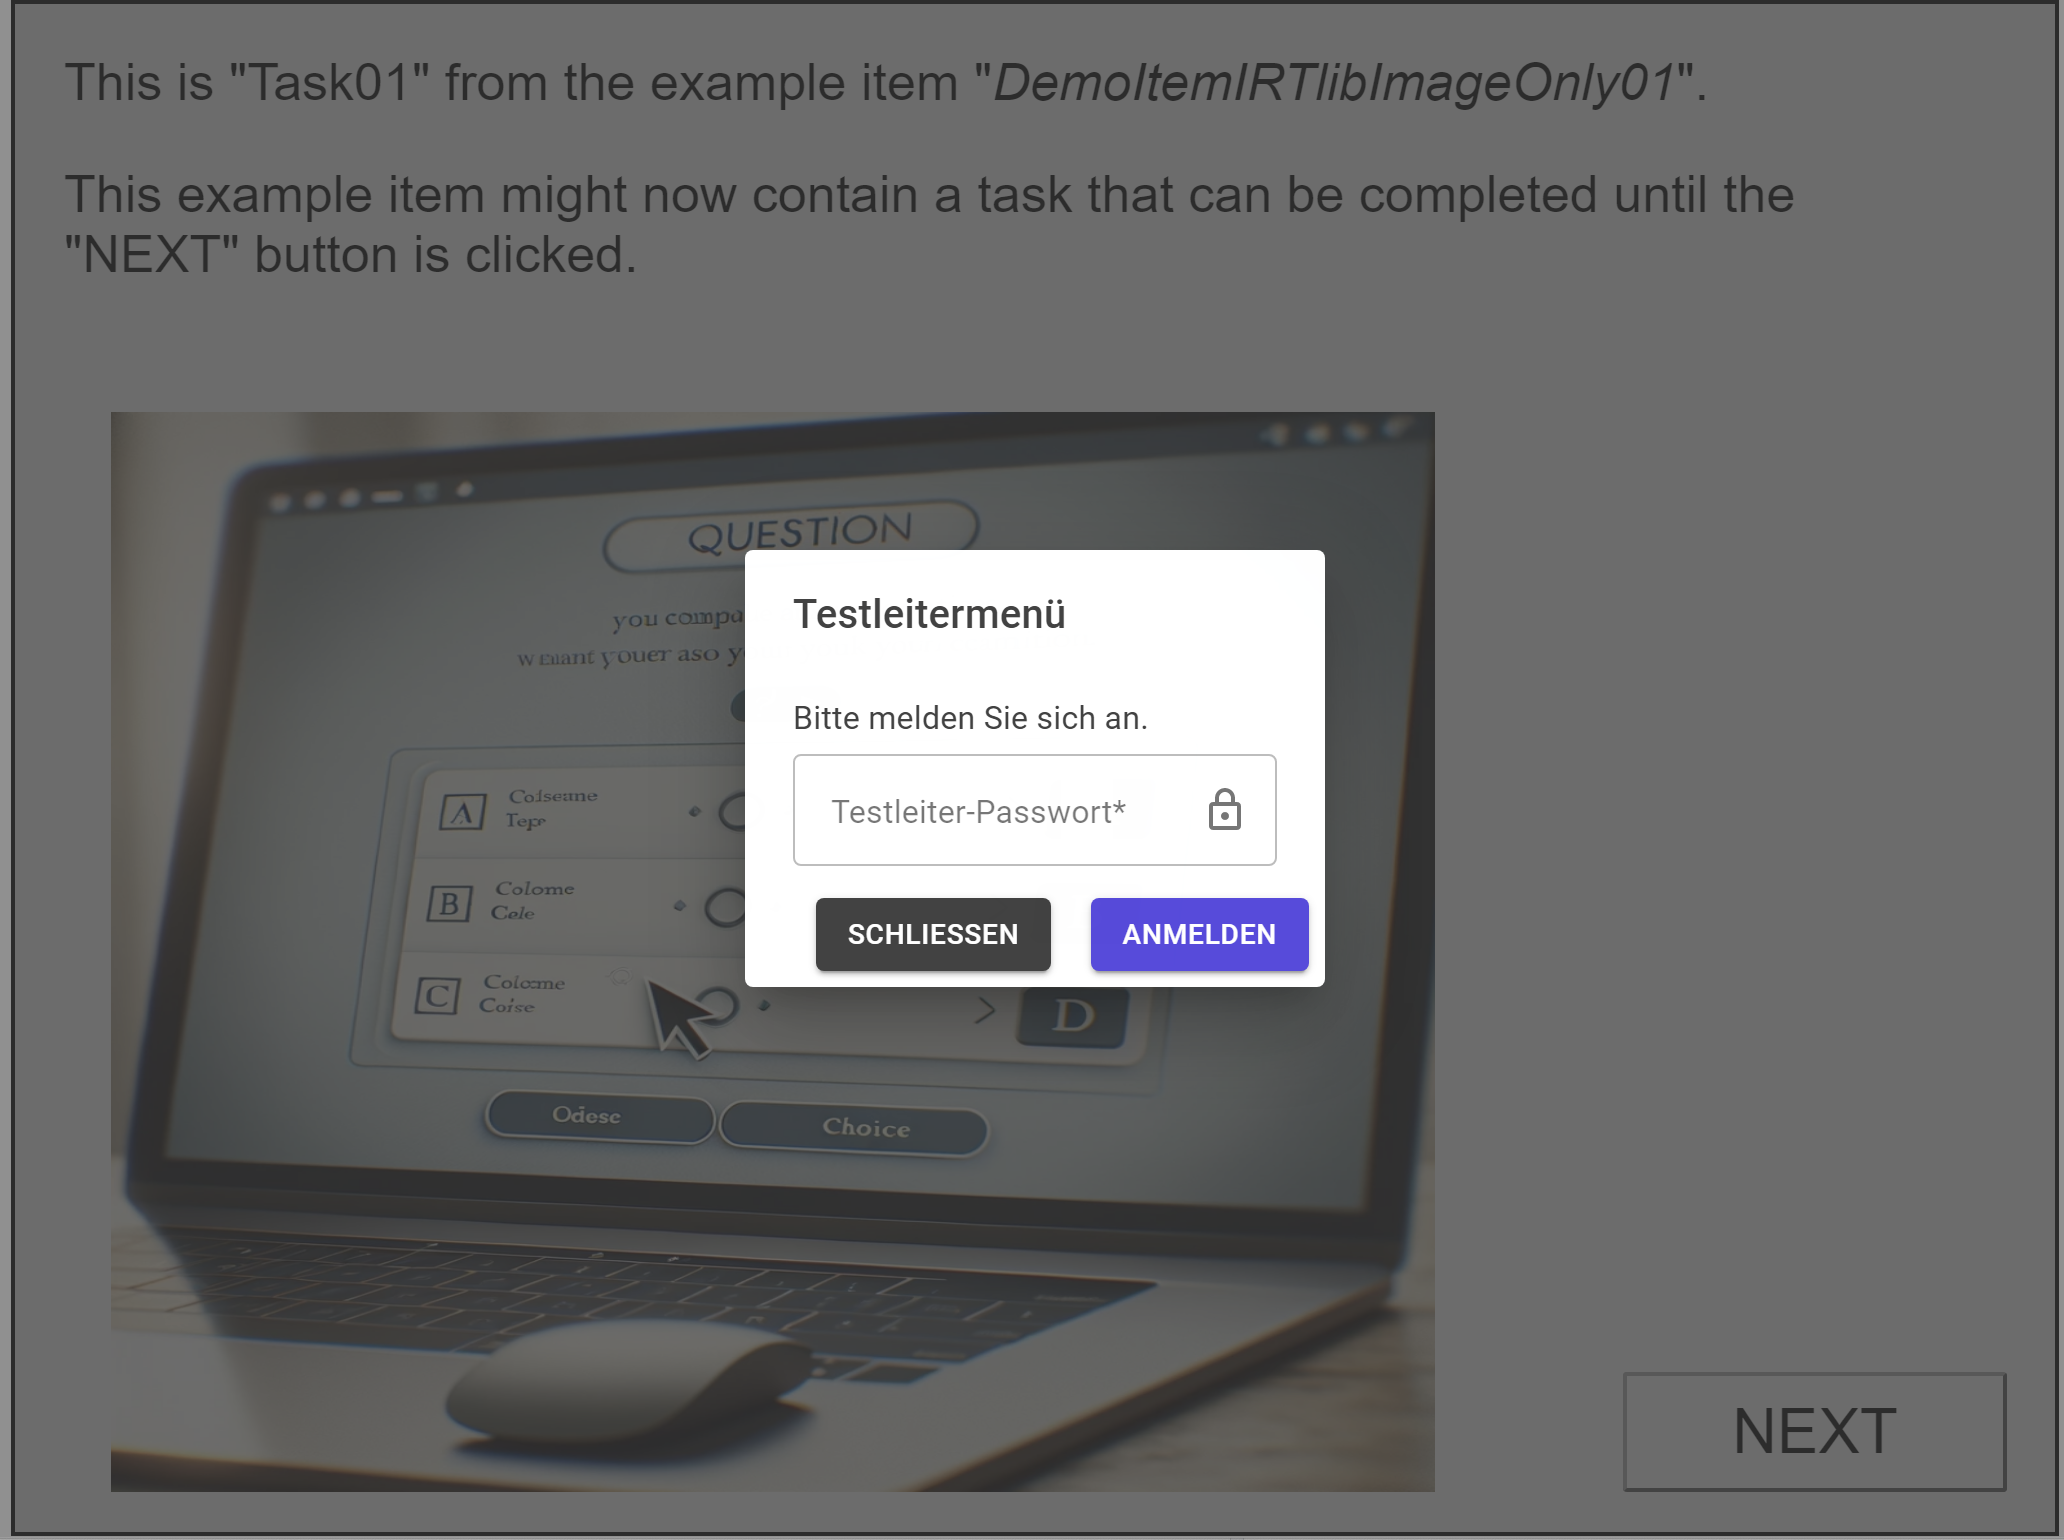
\includegraphics[width=0.8\textwidth,height=\textheight]{img/screenshot-test-adminstrator-menue-password-example-01-DEU.png}

Welche Funktionen nun wirklich zugreifbar sind wird dadurch gesteuert,
welches Passwort eingegeben wird. Nur wenn ein gültige Passwort bekannt
ist, können Funktionen der Testleitung aufgerufen werden.

Beispiel:

\begin{itemize}
\tightlist
\item
  In der folgenden Konfiguration können Testleiter mit diesem Passwort
  zur nächaten Aufgaben springen (\emph{Weiter}) oder die Anwendung
  beenden (\emph{Sitzung beenden}):
\end{itemize}

\begin{quote}
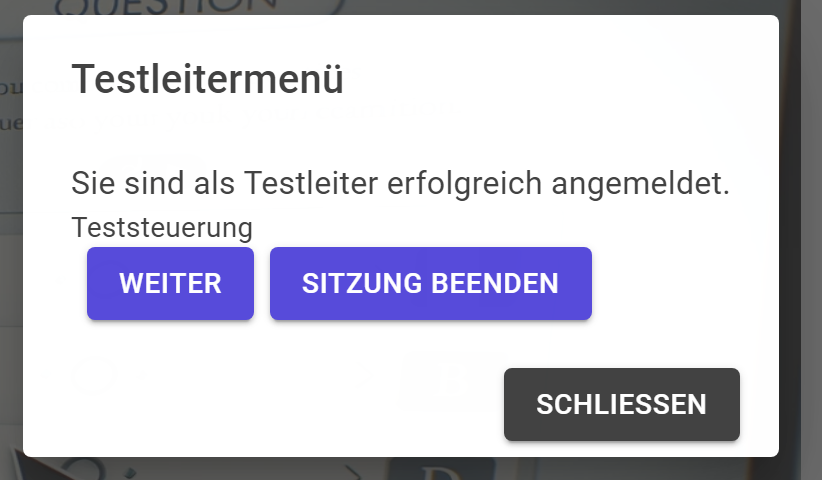
\includegraphics[width=2.60417in,height=\textheight]{img/screenshot-test-adminstrator-menue-two-functions-example-01-DEU.png}
\end{quote}

\begin{quote}
Um eine Rolle zu definieren, muss zunächst das \texttt{+}-Symbol unten
rechts geklickt werden. Danach kann der Name einer Rolle und ein
Passwort definiert:
\end{quote}

\begin{quote}
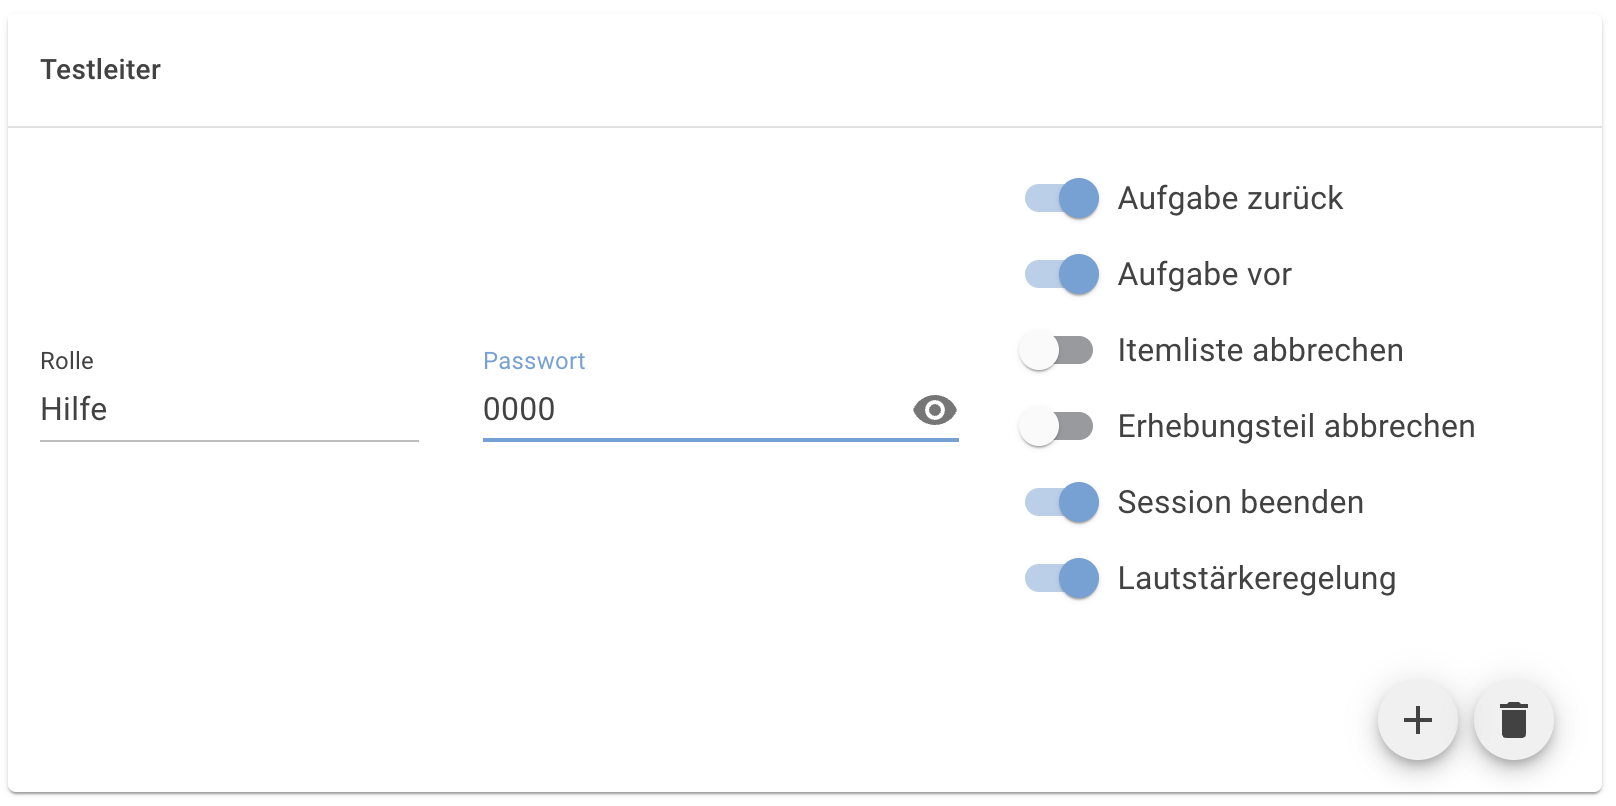
\includegraphics[width=4.6875in,height=\textheight]{img/screenshot-test-adminstrator-menue-example-configuration-01-DEU.png}
\end{quote}

\begin{quote}
Der Name der Rolle dient nur der Dokumentation. Entscheidend für die
Funktionalität ist die Vergabe eines eindeutigen Passwortes und die
Auswahl einer oder mehrerer der folgenden Funktionen:
\end{quote}

\begin{itemize}
\tightlist
\item
  \textbf{Aufgabe zurück}: Ermöglicht die Navigation zur vorherigen
  Aufgabe.
\item
  \textbf{Aufgabe vor}: Ermöglicht die Navigation zur nächsten Aufgabe
  an.
\item
  \textbf{Itemliste abbrechen}: Ermöglicht die Abarbeitung der aktuellen
  Itemliste abzubrechen. Diese Option ist insbesondere sinnvoll, wenn in
  einem \emph{Erhebungsteil} die Option \emph{Routing} aktiviert ist und
  die Definition von \emph{CBA ItemBuilder} Tasks mit Hilfe von
  Itemlisten umgesetzt ist.\\
\item
  \textbf{Erhebungsteil abbrechen}: Ermöglicht den Abbruch des aktuellen
  Erhebungsteils.
\item
  \textbf{Sitzung beenden}: Ermöglicht das Beenden der aktuellen
  Sitzung.
\item
  \textbf{Lautstärkeregelung}: Ermöglicht die Änderung der Lautstärke.
\end{itemize}

Die Audiodatei, welche zur Kontrolle der Audioausgabe abgespielt wird
nachdem die Lautstärke verändert wurde, kann im Abschnitt \emph{Audio
für Soundtest} eingefügt und in der Studienkonfiguration hinterlegt
werden.

Wenn geänderte Einstellungen erhalten bleiben sollen müssen die
Änderungen über das Disketten-Symbol gespeichert werden. Andernfalls
kann das Verwerfen-Symbol verwendet werden:

\begin{figure}[H]


\includegraphics[width=1.25in,height=\textheight]{img/screenshot-icons-undo-and-save-01.png} \hfill{}

\end{figure}

\end{tcolorbox}

\hypertarget{abschluss-von-erhebungen-1}{%
\section{Abschluss von Erhebungen}\label{abschluss-von-erhebungen-1}}

Für die Integration von Assessments in externe Abläufe besteht die
Möglichkeit zu konfiguriere, wie nach der Bearbeitung der
Assessmentinhalte in einer \emph{Session} vorgegangen werden soll, was
also am \emph{Session-Ende} geschehen wird.

\begin{tcolorbox}[enhanced jigsaw, colbacktitle=quarto-callout-tip-color!10!white, coltitle=black, colframe=quarto-callout-tip-color-frame, leftrule=.75mm, breakable, opacitybacktitle=0.6, toprule=.15mm, title=\textcolor{quarto-callout-tip-color}{\faLightbulb}\hspace{0.5em}{Eingebettete Programmhilfe}, colback=white, titlerule=0mm, arc=.35mm, bottomtitle=1mm, toptitle=1mm, rightrule=.15mm, bottomrule=.15mm, left=2mm, opacityback=0]

\hypertarget{session-und-session-ende-1}{%
\subsection{Session und Session-Ende}\label{session-und-session-ende-1}}

Eine \emph{Session} bezieht sich auf die Durchführung einer Erhebung mit
\emph{einer} Person zu \emph{einem} bestimmten Zeitpunkt. Der in einer
Session angezeigte Inhalt entspricht einer konfigurierten \emph{Studie},
wie sie im \emph{IRTlib Editor} erstellt werden kann. Nachdem alle in
einer \emph{Studie} definierten Erhebungsteile durchgeführt worden sind,
wird das \emph{Session-Ende} erreicht.

\hypertarget{konfiguration-des-session-endes-1}{%
\subsubsection{Konfiguration des
Session-Endes}\label{konfiguration-des-session-endes-1}}

Was nach einem \emph{Session-Ende} erfolgt, d.h. wie sich der
\emph{IRTlib Players} am Ende einer Sitzung verhält, kann mit den
folgenden Optionen festgelegt werden:

\begin{itemize}
\item
  \textbf{Neue Session starten}: Es wird eine neue Sitzung gestartet.
  Deses Verhalten ist nicht sinnvoll, wenn die Anmeldedaten übergeben
  werde (entweder als \emph{Startup-Parameter} oder als
  \emph{URL-Parameter}).
\item
  \textbf{Endtext anzeigen}: Wenn diese Option ausgewählt ist, zeigt die
  Plattform den konfigurierten Text an. Der Text kann als
  \emph{Nachricht auf Endseite} konfiguirert werden.
\item
  \textbf{End-Item anzeigen}: Analog zu einem \emph{Login-Item} kann
  auch ein \emph{CBA ItemBuilder}-Item definiert werden, das am Ende
  einer Sitzung angezeigt wird.
\end{itemize}

\begin{quote}
Das \emph{End-Item} kann schließlich das Beenden des
Offline-\emph{IRTlib Players} anstoßen. Ein Beispiel für ein
\emph{End-Item} mit dem notwendigen JavaScript-Aufruf findet sich
\href{https://kroehne.github.io/CBAItemBuilderBook/items/9_09/IRTLibEndItemExample.zip}{hier}.
\end{quote}

\begin{itemize}
\tightlist
\item
  \textbf{Redirect to Exit URL (Redirct zu Exit-Url)}: Bei
  Online-Lieferungen mit dem \emph{IRTlib Player} ist es möglich, auf
  eine URL umzuleiten. Die \emph{Weiterleitungs-URL} kann dann
  konfiguriert werden.
\end{itemize}

\hypertarget{weitere-optionen-1}{%
\subsubsection{Weitere Optionen}\label{weitere-optionen-1}}

\begin{itemize}
\tightlist
\item
  \textbf{Session ID kann wiederverwendet werden}: Wenn diese Option
  aktiviert ist, können mehrere Datenerfassungen mit einer Session-ID
  administriert werden.
\end{itemize}

Wenn geänderte Einstellungen erhalten bleiben sollen müssen die
Änderungen über das Disketten-Symbol gespeichert werden. Andernfalls
kann das Verwerfen-Symbol verwendet werden:

\begin{figure}[H]


\includegraphics[width=1.25in,height=\textheight]{img/screenshot-icons-undo-and-save-01.png} \hfill{}

\end{figure}

\end{tcolorbox}

\bookmarksetup{startatroot}

\hypertarget{vorbereitung-erhebungsteile}{%
\chapter{Vorbereitung:
Erhebungsteile}\label{vorbereitung-erhebungsteile}}

\let\clearpage\standardclearpage

\bookmarksetup{startatroot}

\hypertarget{vorbereitung-erhebungsteile-1}{%
\chapter{Vorbereitung:
Erhebungsteile}\label{vorbereitung-erhebungsteile-1}}

Assessments, die mit der \emph{IRTlib Software} administriert werden
bestehen aus sogenannten \emph{Erehebungsteilen}. Nach der Konfiguration
einer Studie muss zumindest ein \emph{Erhebungsteil} angelegt werden.

\hypertarget{erhebungsteilverwaltung-1}{%
\section{Erhebungsteilverwaltung}\label{erhebungsteilverwaltung-1}}

Nach dem Erstellen einer \emph{Studie} erfolgt in der Ansicht
\emph{Erhebungsteile} als nächster Schritt zur Vorbereitung einer
Testauslifierung das \textbf{Hinzufügen eines neuen Erhebungsteils}:

\url{https://youtu.be/YFgu8uz8nkc}

Die erstellten \emph{Erhebungsteile} erscheinen als Karten in der
Ansicht \emph{Erhebungsteile}. Wenn Studien aus mehreren Erhebunsteilen
bestehen, kann für \emph{lineare Abläufe} die Reihenfolge der
Erhebungsteile in der Ansichht \emph{Erhebungsteile} / \emph{Übersicht}
angepasst werden. Sollen \emph{Erhebungsteile} in Abhängigkeit von
Variablen (z.B. übergebene \emph{Preload}-Variablen oder andere
\emph{Blockly}-Variablen gesteuert werden, kann alternativ ein Routing
zwischen Erhebungsteilen konfiguriert werden.

Eine detaillierte Anleitung zur Erstellung von \emph{Erhebungsteilen}
findet sich hier in der eingebetteten Hilfe:

\begin{tcolorbox}[enhanced jigsaw, colbacktitle=quarto-callout-tip-color!10!white, coltitle=black, colframe=quarto-callout-tip-color-frame, leftrule=.75mm, breakable, opacitybacktitle=0.6, toprule=.15mm, title=\textcolor{quarto-callout-tip-color}{\faLightbulb}\hspace{0.5em}{Eingebettete Programmhilfe}, colback=white, titlerule=0mm, arc=.35mm, bottomtitle=1mm, toptitle=1mm, rightrule=.15mm, bottomrule=.15mm, left=2mm, opacityback=0]

\hypertarget{erhebungsteil-anlegen-1}{%
\subsection{Erhebungsteil Anlegen}\label{erhebungsteil-anlegen-1}}

Mit dem \emph{IRTLib Editor} werden Konfigurationen für \emph{Studien}
erstellt, welche dann in einem \emph{IRTLib Player} zur Durchführung
computerbasierter Assessments verwendet werden können. \emph{Studie}
bestehen aus einem oder mehreren \emph{Erhebungsteilen}.

\hypertarget{wie-gehts-1}{%
\subsubsection{Wie geht's?}\label{wie-gehts-1}}

Nachdem eine \emph{Studie} angelegt ist, kann nun über Plus-Icon unten
rechts ein \emph{Erhebungsteil} hinzugefügt werden:

\begin{figure}[H]


\includegraphics[width=0.52083in,height=\textheight]{img/icon-plus.png} \hfill{}

\end{figure}

Danach geben Sie bitte in dem Dialog \textbf{Neuen Erhebungsteil
erstellen} eine \emph{Bezeichnung} und optional eine \emph{Beschreibung}
ein.

Achten Sie darauf, dass für die \emph{Bezeichnung} wieder nur Buchstaben
(Groß und Kleinschreibung), Ziffer und ein \texttt{\_} erlaubt sind.

Klicken Sie anschließend auf \emph{Speichern}.

\begin{figure}[H]

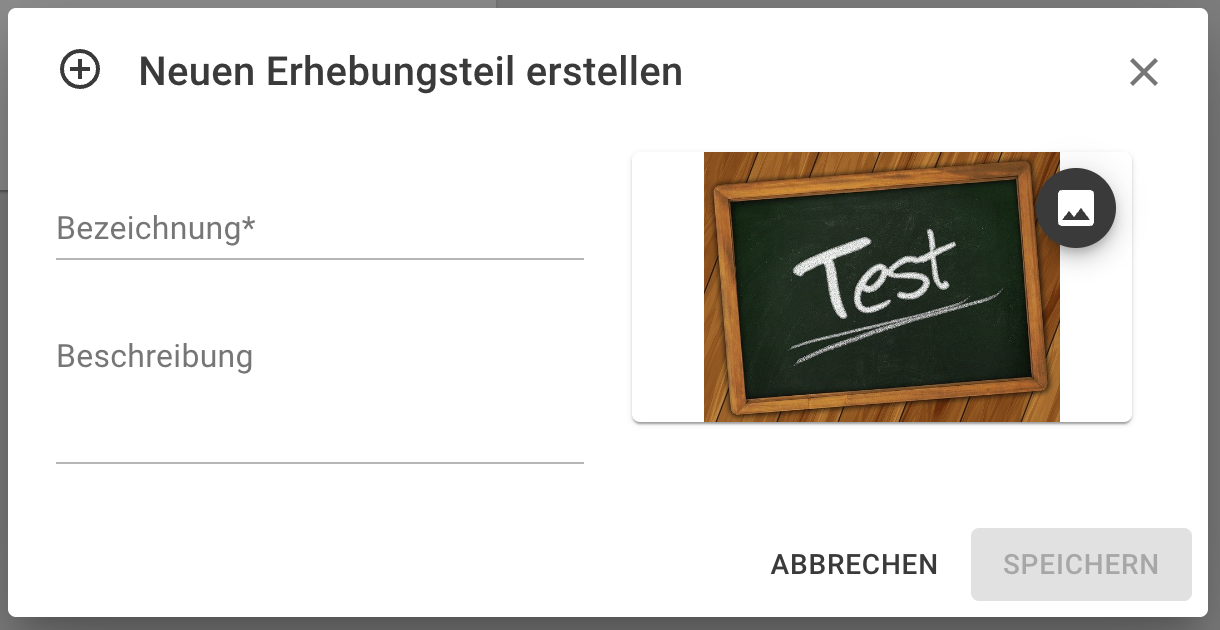
\includegraphics[width=4.16667in,height=\textheight]{img/screenshot-new-study-part-empty-DEU.png} \hfill{}

\end{figure}

Bei Bedarf können Sie über das folgende Icon einem \emph{Erhebungsteil}
auch ein Bild zuordnen. Dieses Bild wird im \emph{IRTLib Editor} für
diesen Erhebungsteil verwendet:

\begin{figure}[H]


\includegraphics{img/icon-study-image.png} \hfill{}

\end{figure}

\hypertarget{erhebungsteil-bearbeiten-1}{%
\subsubsection{Erhebungsteil
Bearbeiten}\label{erhebungsteil-bearbeiten-1}}

Erstellten \emph{Erhebungsteile} werden in der Erhebungsteilübersicht
als Kacheln angezeigt:

\begin{figure}[H]

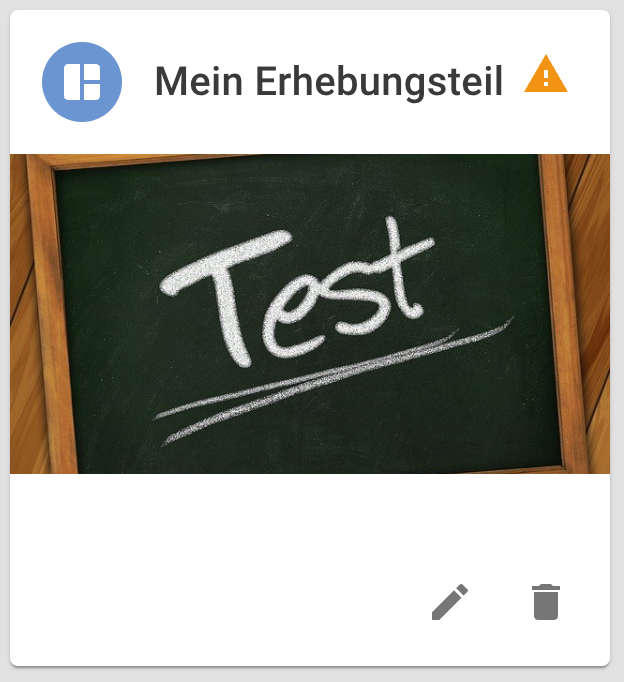
\includegraphics[width=3.125in,height=\textheight]{img/screenshot-new-study-part-card.DEU.png} \hfill{}

\end{figure}

\begin{itemize}
\tightlist
\item
  Um nun mit der Konfiguration eines \emph{Erhebungsteils} fortzufahren,
  klicken Sie auf das kleine Bearbeiten-Icon:
\end{itemize}

\begin{figure}[H]


\includegraphics{img/icon-edit.png} \hfill{}

\end{figure}

\begin{itemize}
\tightlist
\item
  \textbf{Erhebungsteil Löschen}: Mit dem Papierkorb-Icon können Sie
  \emph{Erhebungsteile} auch wieder löschen. Das Löschen von
  \emph{Erhebungsteilen} kann nicht rückgängig gemacht werden:
\end{itemize}

\begin{figure}[H]


\includegraphics{img/icon-delete.png} \hfill{}

\end{figure}

\hypertarget{erhebungsteile-sortieren-1}{%
\subsubsection{Erhebungsteile
Sortieren}\label{erhebungsteile-sortieren-1}}

Wenn in der Konfiguration einer \emph{Studie} in der Ansicht \emph{Info}
(Abschnitt \emph{Übersicht}) die Option \emph{Routing für Erhebungsteile
aktivieren} nicht ausgewählt ist, dann werden \emph{Erhebungsteile} in
der Reihenfolge administriert, in welcher sie in der
Erhebungsteilverwaltung angezeigt werden.

\begin{itemize}
\tightlist
\item
  \textbf{Erhebungsteile Verschieben}: Um per drag-and-drop die
  Reihenfolge von \emph{Erhebungsteilen} zu verändern, muss zunächst
  über folgendes Toggle-Icon der Modus \emph{Reihenfolge Ändern}
  aktiviert werden:
\end{itemize}

\begin{figure}[H]


\includegraphics[width=0.52083in,height=\textheight]{img/icon-toggle.png} \hfill{}

\end{figure}

\begin{quote}
Danach können die Kacheln in die gewünschte Reihenfolge gebracht werden.
Der Modus \emph{Reihenfolge Ändern} wird beendet, wenn das
Disketten-Symbol angeklickt oder die Änderungen verworfen werden:
\end{quote}

\begin{figure}[H]


\includegraphics[width=1.25in,height=\textheight]{img/screenshot-icons-undo-and-save-01.png} \hfill{}

\end{figure}

\end{tcolorbox}

Die Reihenfolge von \emph{Erhebunsteilen} kann in der Ansicht
\emph{Erhebungsteile} verändert werden:

\url{https://youtu.be/Ag0IcETZTdM}

Vor dem Hinzufügen bzw. Auswählen von CBA ItemBuilder Projekten, sie im
Abschnitt Assessmentinhalte (Items) beschrieben, können in der Ansicht
\emph{Info} ausgewählte Eintsellungen konfiguriert werden.

Eine detaillierte Beschreibung der findet sich hier in der eingebetteten
Hilfe:

\begin{tcolorbox}[enhanced jigsaw, colbacktitle=quarto-callout-tip-color!10!white, coltitle=black, colframe=quarto-callout-tip-color-frame, leftrule=.75mm, breakable, opacitybacktitle=0.6, toprule=.15mm, title=\textcolor{quarto-callout-tip-color}{\faLightbulb}\hspace{0.5em}{Eingebettete Programmhilfe}, colback=white, titlerule=0mm, arc=.35mm, bottomtitle=1mm, toptitle=1mm, rightrule=.15mm, bottomrule=.15mm, left=2mm, opacityback=0]

\hypertarget{grundkonfiguration-fuxfcr-erhebungsteile-1}{%
\subsection{Grundkonfiguration für
Erhebungsteile}\label{grundkonfiguration-fuxfcr-erhebungsteile-1}}

\hypertarget{bezeichnung-und-beschreibung-1}{%
\subsubsection{Bezeichnung und
Beschreibung}\label{bezeichnung-und-beschreibung-1}}

\begin{itemize}
\item
  \textbf{Bezeichnung}: Die interne Bezeichnung des Erhebungsteils,
  welche im \emph{IRTlib Editor} zur Bearbeitung und zur Definition des
  Ablaufs angezeigt wird. Bezeichnungen dürfen keine Sonderzeichen,
  Leerzeichen und Umlaute enthalten und nicht mit einer Ziffer beginnen.
\item
  \textbf{Beschreibung}: Optionale zusätzliche Beschreibung eines
  Erhebungsteils.
\end{itemize}

\hypertarget{routing-innerhalb-von-erhebungsteilen-2}{%
\subsubsection{Routing innerhalb von
Erhebungsteilen}\label{routing-innerhalb-von-erhebungsteilen-2}}

\begin{itemize}
\tightlist
\item
  \textbf{Routing aktivieren}: Die konfigurierten Assessmentinhalte im
  Abschnitt \emph{Items} können als lineare Sequenz, d.h. in der
  konfigurierten Reihenfolge administriert werden. Soll eine davon
  abweichende Reihenfolge verwendet werden, kann hier die Option
  \emph{Routing aktivieren} gewählt werden. Die Reihenfolge kann dann im
  Abschnitt \emph{Routing} als visuelles Programm spezifziert werden.
\end{itemize}

\hypertarget{weitere-einstellungen-5}{%
\subsubsection{Weitere Einstellungen}\label{weitere-einstellungen-5}}

\begin{itemize}
\tightlist
\item
  \textbf{Snapshot verwenden}: Damit CBA ItemBuilder \emph{Tasks}
  mehrfach besucht werden können, wird deren Inhalt beim Verlassen des
  Items in sogenannten \emph{Snapshots} gespeichert. \emph{Snapshots}
  können auch dazu verwendet werden, um die Inhalte eines CBA
  ItemBuilder \emph{Tasks} zu einem späteren Zeitpunkt erneut
  darzustellen. Diese Option sollte nur dann deaktiviert werden, wenn es
  einen gewichtigen Grund gibt und die Konsequenzen (d.h. die dann nicht
  gespeicherten \emph{Snapshot}-Daten) sorgfältig bedacht wurden.
\end{itemize}

\end{tcolorbox}

Das Hinzufügen und Verwalten von CBA ItemBuilder Projekte innerhalb des
\emph{IRTlib-Editors} erfolgt im Abschnitt Items.

\begin{tcolorbox}[enhanced jigsaw, colbacktitle=quarto-callout-caution-color!10!white, coltitle=black, colframe=quarto-callout-caution-color-frame, leftrule=.75mm, breakable, opacitybacktitle=0.6, toprule=.15mm, title=\textcolor{quarto-callout-caution-color}{\faFire}\hspace{0.5em}{Hinweis zur Zeitbegrenzung}, colback=white, titlerule=0mm, arc=.35mm, bottomtitle=1mm, toptitle=1mm, rightrule=.15mm, bottomrule=.15mm, left=2mm, opacityback=0]

Für die Administration von zeitbegrenzten Erhebungsteilen kann unter
Bearbeitungszeit ein Zeitlimit definiert werden. Wenn die Option
\emph{Bearbeitungszeit begrenzen} aktiviert ist, können ein oder mehere
\emph{Tasks} definiert werden, welche bei einem \emph{Timeout} angezeigt
werden. Außerdem können im Abschnitt Vorspann-Items(s) und
Nachspann-Item(s) Inhalte definiert werden, welche vor bzw. nach dem
zeitbegrenzten Teil administriert werden.

\end{tcolorbox}

\hypertarget{assessmentinhalte-items-einfuxfcgen-1}{%
\section{Assessmentinhalte (Items)
Einfügen}\label{assessmentinhalte-items-einfuxfcgen-1}}

Die Inhalte, welche in einem Erhebungsteil vom Typ \emph{CBA
ItemBuilder} verwendet werden sollen, werden über den \emph{IRTlib
Editor} in die Konfiguration übernommen, d.h. die mit dem \emph{IRTlib
Editor} erstellte Konfiguration enthält auch die \emph{CBA ItemBuilder}
\emph{Project Files}. Für das Hinzufügen oder Aktualisierung von
\emph{CBA ItemBuilder} Projekten steht die Ansicht \emph{Items} zur
Verfügung.

Eine detaillierte Beschreibung der findet sich hier in der eingebetteten
Hilfe:

\begin{tcolorbox}[enhanced jigsaw, colbacktitle=quarto-callout-tip-color!10!white, coltitle=black, colframe=quarto-callout-tip-color-frame, leftrule=.75mm, breakable, opacitybacktitle=0.6, toprule=.15mm, title=\textcolor{quarto-callout-tip-color}{\faLightbulb}\hspace{0.5em}{Eingebettete Programmhilfe}, colback=white, titlerule=0mm, arc=.35mm, bottomtitle=1mm, toptitle=1mm, rightrule=.15mm, bottomrule=.15mm, left=2mm, opacityback=0]

\hypertarget{items-konfigurieren-1}{%
\subsection{Items Konfigurieren}\label{items-konfigurieren-1}}

\hypertarget{grundfunktionen-1}{%
\subsubsection{Grundfunktionen}\label{grundfunktionen-1}}

\begin{itemize}
\tightlist
\item
  \textbf{Importieren von \emph{CBA ItemBuilder}-Projektdateien}: Der
  \emph{IRTlib Editor} pflegt eine \emph{Liste bekannter Items}, zu
  denen \emph{CBA ItemBuilder}-Projekdateien die noch nicht bekannt sind
  hinzugefügt werden können. Um eine Projektdatei hinzuzufügen, öffnet
  man zunächst mit dem \texttt{+}-Symbol die \emph{Liste bekannter
  Items} und wählt dann die Schaltfläche \emph{Imporiteren} aus.
\end{itemize}

\begin{figure}[H]


\includegraphics[width=0.41667in,height=\textheight]{img/screenshot-add-project-plus-icon.png} \hfill{}

\end{figure}

\begin{figure}[H]


\includegraphics[width=1.25in,height=\textheight]{img/screenshot-import-items-button-01.png} \hfill{}

\end{figure}

\begin{itemize}
\tightlist
\item
  \textbf{Aktualisieren bereits importiereter \emph{CBA
  ItemBuilder}-Projektdateien}: Wenn eine \emph{CBA
  ItemBuilder}-Projektdatei bereits in der \emph{Liste der bekannten
  Items} enthalten ist, können die Projektdateien aktualisiert werden.
  Sie werden dann nicht zusätzlich zur \emph{Liste der bekannten Items}
  hinzugefügt, sondern die bereits vorhandene \emph{CBA
  ItemBuilder}-Projektdatei wird in einer neueren Version hinterlegt. Um
  ein Item zu aktualisieren muss es zunächst in der Liste der Items
  eines \emph{Erhebungsteils} ausgewählt werden. Dadurch wird das
  Aktualisieren-Symbol aktiv. In dem sich dann öffnenenden Dialog
  \emph{Item aktualisieren} kann über die Schaltfläche
  \emph{Imporiteren} eine aktualisierte Version einer \emph{CBA
  ItemBuilder}-Projektdatei hinzugefügt werden.
\end{itemize}

\begin{figure}[H]


\includegraphics[width=0.41667in,height=\textheight]{img/screenshot-update-item-icon-01.png} \hfill{}

\end{figure}

\begin{figure}[H]


\includegraphics[width=1.25in,height=\textheight]{img/screenshot-import-items-button-01.png} \hfill{}

\end{figure}

\begin{itemize}
\tightlist
\item
  \textbf{Vorschau von \emph{CBA ItemBuilder}-Projektdateien}: Die in
  einem \emph{Erhebungsteil} hinzugefügten Items können direkt im
  \emph{IRTlib Editor} in einer eingebauten Preview-Funktion angesehen
  werden. Um ein Item zu anzusehen muss es zunächst in der Liste der
  Items eines \emph{Erhebungsteils} ausgewählt werden. Danach kann die
  \emph{Vorschau} über das Augen-Symbol aufgerufen werden:
\end{itemize}

\begin{figure}[H]


\includegraphics[width=0.41667in,height=\textheight]{img/screenshot-preview-icon-01.png} \hfill{}

\end{figure}

\begin{itemize}
\tightlist
\item
  \textbf{Exportieren von \emph{CBA ItemBuilder}-Projektdateien}:
  \emph{CBA ItemBuilder}-Projektdateien die in den \emph{IRTlib Editor}
  importiert wurden, können zur weiteren Bearbeitung mit dem \emph{CBA
  ItemBuilder} exportiert werden. Um ein ausgewhähltes Item aus der
  Liste der Items eines \emph{Erhebungsteils} zu exportieren, kann das
  Download-Symbol augerufen werden:
\end{itemize}

\begin{figure}[H]


\includegraphics[width=0.41667in,height=\textheight]{img/screenshot-download-item-icon-01.png} \hfill{}

\end{figure}

\begin{itemize}
\tightlist
\item
  \textbf{Löschen von \emph{CBA ItemBuilder}-Projektdateien}: Die in
  \emph{Erhebungsteilen} eingefügten Items können aus einem
  \emph{Erhebungsteil} wieder gelöscht werden. Durch das Löschen-Symbol
  wird das Item aus einem \emph{Erhebungsteil} entfernt, es verbleibt
  aber in der \emph{Liste bekannter Items}:
\end{itemize}

\begin{figure}[H]


\includegraphics[width=0.41667in,height=\textheight]{img/screenshot-delete-item-icon-01.png} \hfill{}

\end{figure}

\begin{quote}
Hinweis: Es ist bisher nicht möglich, \emph{CBA
ItemBuilder}-Projektdateien aus der \emph{Liste bekannter Items} wieder
zu löschen. Diese Funktionalität ist nicht notwendig, da \emph{CBA
ItemBuilder}-Projektdateien vom \emph{IRTlib-Editor} nur dann in die
Konfiguration einer \emph{Studie} übernommen werden, wenn \emph{Tasks}
aus einer \emph{CBA ItemBuilder}-Projektdatei in einem
\emph{Erhebungsteil} verwendet werden.
\end{quote}

\hypertarget{sortieren-von-items-linearer-ablauf-1}{%
\subsubsection{Sortieren von Items (Linearer
Ablauf)}\label{sortieren-von-items-linearer-ablauf-1}}

\begin{itemize}
\tightlist
\item
  \textbf{Sortieren \emph{CBA ItemBuilder}-Projektdateien}: Wenn für
  einen \emph{Erhebungsteil} die Option \emph{Routing aktivieren} nicht
  ausgewählt ist, dann kann in der Liste der Items die Reihenfolge über
  die folgenden Schaltfläche angepasst werden:
\end{itemize}

\begin{figure}[H]


\includegraphics[width=0.83333in,height=\textheight]{img/screenshot-sort-items-icon-01.png} \hfill{}

\end{figure}

\begin{quote}
Die Items dann exakt so administriert, wie sie für einen
\emph{Erhebungsteil} in dieser Liste aufgeführt sind.
\end{quote}

Hinweis: Änderungen an der Sicht \emph{Items} müssen über das
Disketten-Symbol gespeichert oder mit dem Rückgängig-Symbol verwerfen
werden:

\begin{figure}[H]


\includegraphics[width=1.25in,height=\textheight]{img/screenshot-icons-undo-and-save-01.png} \hfill{}

\end{figure}

\end{tcolorbox}

\hypertarget{bearbeitungszeit-1}{%
\section{Bearbeitungszeit}\label{bearbeitungszeit-1}}

Wenn die Administration einer linearen Folge von \emph{CBA ItemBuilder}
\emph{Tasks} mit einer begrenzten Bearbeitungszeit administriert werden
sollen, lässt sich dies durch Definieren einer maximalen
Bearbeitungszeit (in Sekunden) umsetzen. Soll bspw. ein Testinhalt
maximal \emph{28} min. administriert werden, wird als
\emph{Bearbeitungszeit} eine Zeit von \emph{1680} Sekunden definiert.
Die Nachricht, welche beim Ablaufen der Bearbeitungszeit angezeigt
werden soll, lässt sich als ein (oder mehrere) \emph{CBA ItemBuilder}
\emph{Tasks} definieren.

Eine detaillierte Beschreibung der findet sich hier in der eingebetteten
Hilfe:

\begin{tcolorbox}[enhanced jigsaw, colbacktitle=quarto-callout-tip-color!10!white, coltitle=black, colframe=quarto-callout-tip-color-frame, leftrule=.75mm, breakable, opacitybacktitle=0.6, toprule=.15mm, title=\textcolor{quarto-callout-tip-color}{\faLightbulb}\hspace{0.5em}{Eingebettete Programmhilfe}, colback=white, titlerule=0mm, arc=.35mm, bottomtitle=1mm, toptitle=1mm, rightrule=.15mm, bottomrule=.15mm, left=2mm, opacityback=0]

\hypertarget{zeitbegrenzung-definieren-1}{%
\subsection{Zeitbegrenzung
Definieren}\label{zeitbegrenzung-definieren-1}}

\emph{Erhebungsteile} ohne \emph{Routing} können auf einfache Weise
einen zeitbegrenzten Abschnitt enthalten. Dafür wird in der Sicht
\emph{Bearbeitungszeit} die Option \emph{Bearbeitungszeit begrenzen}
aktiviert und ein Zeitlimit in Sekunden (\textgreater0) eingetragen.

Für eine Zeitbegrenzung werden vier Gruppen von \emph{CBA ItemBuilder}
\emph{Tasks} unterschieden, die an unterschiedlichen Stellen im
\emph{IRTlib Editor} definiert werden. In der Sicht \emph{Items} (analog
zu nicht zeitbegrenzten \emph{Erhebungsteilen}) werden die Items für
welche die Zeitbegrenzug gelten soll definiert:

\begin{itemize}
\tightlist
\item
  \textbf{Items}: Items die so lange angezeigt werden, bis das Zeitlimit
  erreicht wurde.
\end{itemize}

In der Ansicht \emph{Bearbeitungszeit} kann zusätzlich definiert werden:

\begin{itemize}
\tightlist
\item
  \textbf{Timeout-Items}: Items die nur angezeigt werden, wenn die
  zeitbegrenzten Items nicht in der begrenzten Bearbeitungszeit
  abgeschlossen wurden.
\end{itemize}

Als einzelne Sichten der Konfiguration von \emph{Erhebungsteile} können
schließlich folgende Tasks definiert werden:

\begin{itemize}
\tightlist
\item
  \textbf{Vorspann-Items}: Items die vor dem zeitbegrenzten Abschnitt
  angezeigt werden.
\item
  \textbf{Nachspann-Items}: Items die nach dem zeitbegrenzten Abschnitt
  angezeigt werden.
\end{itemize}

In allen genannten Dialogen stehen die Symbole für folgende Operationen
zur Verfügung:

\begin{itemize}
\tightlist
\item
  Hinzufügen:
  
\includegraphics[width=0.41667in,height=\textheight]{img/screenshot-add-project-plus-icon.png}
\item
  Aktualisieren:
  
\includegraphics[width=0.41667in,height=\textheight]{img/screenshot-update-item-icon-01.png}
\item
  Vorschau/Preview:
  
\includegraphics[width=0.41667in,height=\textheight]{img/screenshot-preview-icon-01.png}
\item
  Download/Export:
  
\includegraphics[width=0.41667in,height=\textheight]{img/screenshot-download-item-icon-01.png}
\item
  Löschen:
  
\includegraphics[width=0.41667in,height=\textheight]{img/screenshot-delete-item-icon-01.png}
\item
  Sortieren:
  
\includegraphics[width=0.83333in,height=\textheight]{img/screenshot-sort-items-icon-01.png}
\end{itemize}

Hinweis: Komplexere Designs mit ggf. mehreren Timern lassen sich mit dem
\emph{IRTlib Editor} umsetzen, wenn die Option \emph{Routing aktivieren}
in der Übersichtsansicht zu einem \emph{Erhebungsteil} aktiviert ist.

Hinweis: Änderungen an der Sicht \emph{Bearbeitungszeit} müssen über das
Disketten-Symbol gespeichert oder mit dem Rückgängig-Symbol verwerfen
werden:

\begin{figure}[H]

\includegraphics[width=1.25in,height=\textheight]{img/screenshot-icons-undo-and-save-01.png} \hfill{}

\end{figure}

\end{tcolorbox}

\begin{tcolorbox}[enhanced jigsaw, colbacktitle=quarto-callout-caution-color!10!white, coltitle=black, colframe=quarto-callout-caution-color-frame, leftrule=.75mm, breakable, opacitybacktitle=0.6, toprule=.15mm, title=\textcolor{quarto-callout-caution-color}{\faFire}\hspace{0.5em}{Vorspann-/Nachspann-Items}, colback=white, titlerule=0mm, arc=.35mm, bottomtitle=1mm, toptitle=1mm, rightrule=.15mm, bottomrule=.15mm, left=2mm, opacityback=0]

Ein zentrales Konzept für die Umsetzung von Zeitbegrenzungen in der
\emph{IRTlib Software} ist die Trennung der zeitbegrenzten Items, und
zusätzlicher Assessmentinhalte, die \emph{vor} oder \emph{nach} dem
zeitbegrenzten Teil administriert werden.

\end{tcolorbox}

\begin{itemize}
\tightlist
\item
  Items die \emph{nach} einem potentiell Zeitbegrenzten Abschnitt eines
  Erhebugnsteils administriert werde, werden als \emph{Nachspann-Items}
  bezeichnet.
\end{itemize}

\begin{tcolorbox}[enhanced jigsaw, colbacktitle=quarto-callout-tip-color!10!white, coltitle=black, colframe=quarto-callout-tip-color-frame, leftrule=.75mm, breakable, opacitybacktitle=0.6, toprule=.15mm, title=\textcolor{quarto-callout-tip-color}{\faLightbulb}\hspace{0.5em}{Eingebettete Programmhilfe}, colback=white, titlerule=0mm, arc=.35mm, bottomtitle=1mm, toptitle=1mm, rightrule=.15mm, bottomrule=.15mm, left=2mm, opacityback=0]

\hypertarget{items-nach-einer-zeitebgrenzung-1}{%
\subsection{Items nach einer
Zeitebgrenzung}\label{items-nach-einer-zeitebgrenzung-1}}

Der \emph{Erhebungsteile} erlauben die Definition von Items in
verschiedenen Abschnitten. Items in diesem Abschnitt
\emph{Nachspann-Item(s)} werden nach den Items angezeigt, welche im
Abschnitt \emph{Items} eines \emph{Erhebungsteils} definiert sind. Die
Trennung in \emph{Nachspann-Item(s)} und \emph{Items} ist besonders
sinnvoll, wenn unter \emph{Bearbeitungszeit} eine Zeitbegrenzung
aktiviert ist.

Um Items in dem Abschnitt \emph{Nachspann-Item(s)} zu konfigurieren
stehen die folgenden Optionen zur Verfügung:

\begin{itemize}
\tightlist
\item
  Hinzufügen:
  \includegraphics[width=0.41667in,height=\textheight]{img/screenshot-add-project-plus-icon.png}
\item
  Aktualisieren:
  \includegraphics[width=0.41667in,height=\textheight]{img/screenshot-update-item-icon-01.png}
\item
  Vorschau/Preview:
  \includegraphics[width=0.41667in,height=\textheight]{img/screenshot-preview-icon-01.png}
\item
  Download/Export:
  \includegraphics[width=0.41667in,height=\textheight]{img/screenshot-download-item-icon-01.png}
\item
  Löschen:
  \includegraphics[width=0.41667in,height=\textheight]{img/screenshot-delete-item-icon-01.png}
\item
  Sortieren:
  \includegraphics[width=0.83333in,height=\textheight]{img/screenshot-sort-items-icon-01.png}
\end{itemize}

Hinweis: Änderungen an der Sicht \emph{Nachspann-Item(s)} müssen über
das Disketten-Symbol gespeichert oder mit dem Rückgängig-Symbol
verwerfen werden:

\begin{figure}[H]

\includegraphics[width=1.25in,height=\textheight]{img/screenshot-icons-undo-and-save-01.png} \hfill{}

\end{figure}

\end{tcolorbox}

\begin{itemize}
\tightlist
\item
  Items die \emph{vor} einem potentiell Zeitbegrenzten Abschnitt eines
  Erhebugnsteils administriert werde, werden als \emph{Vorspann-Items}
  bezeichnet.
\end{itemize}

\begin{tcolorbox}[enhanced jigsaw, colbacktitle=quarto-callout-tip-color!10!white, coltitle=black, colframe=quarto-callout-tip-color-frame, leftrule=.75mm, breakable, opacitybacktitle=0.6, toprule=.15mm, title=\textcolor{quarto-callout-tip-color}{\faLightbulb}\hspace{0.5em}{Eingebettete Programmhilfe}, colback=white, titlerule=0mm, arc=.35mm, bottomtitle=1mm, toptitle=1mm, rightrule=.15mm, bottomrule=.15mm, left=2mm, opacityback=0]

\hypertarget{items-vor-einer-zeitebgrenzung-1}{%
\subsection{Items vor einer
Zeitebgrenzung}\label{items-vor-einer-zeitebgrenzung-1}}

Der \emph{Erhebungsteile} erlauben die Definition von Items in
verschiedenen Abschnitten. Items in diesem Abschnitt
\emph{Vorspann-Item(s)} werden vor den Items angezeigt, welche im
Abschnitt \emph{Items} eines \emph{Erhebungsteils} definiert sind. Die
Trennung in \emph{Vorspann-Item(s)} und \emph{Items} ist besonders
sinnvoll, wenn unter \emph{Bearbeitungszeit} eine Zeitbegrenzung
aktiviert ist.

Um Items in dem Abschnitt \emph{Vorspann-Item(s)} zu konfigurieren
stehen die folgenden Optionen zur Verfügung:

\begin{itemize}
\tightlist
\item
  Hinzufügen:
  \includegraphics[width=0.41667in,height=\textheight]{img/screenshot-add-project-plus-icon.png}
\item
  Aktualisieren:
  \includegraphics[width=0.41667in,height=\textheight]{img/screenshot-update-item-icon-01.png}
\item
  Vorschau/Preview:
  \includegraphics[width=0.41667in,height=\textheight]{img/screenshot-preview-icon-01.png}
\item
  Download/Export:
  \includegraphics[width=0.41667in,height=\textheight]{img/screenshot-download-item-icon-01.png}
\item
  Löschen:
  \includegraphics[width=0.41667in,height=\textheight]{img/screenshot-delete-item-icon-01.png}
\item
  Sortieren:
  \includegraphics[width=0.83333in,height=\textheight]{img/screenshot-sort-items-icon-01.png}
\end{itemize}

Hinweis: Änderungen an der Sicht \emph{Vorspann-Item(s)} müssen über das
Disketten-Symbol gespeichert oder mit dem Rückgängig-Symbol verwerfen
werden:

\begin{figure}[H]

\includegraphics[width=1.25in,height=\textheight]{img/screenshot-icons-undo-and-save-01.png} \hfill{}

\end{figure}

\end{tcolorbox}

\hypertarget{variablen-1}{%
\section{Variablen}\label{variablen-1}}

\begin{tcolorbox}[enhanced jigsaw, colbacktitle=quarto-callout-important-color!10!white, coltitle=black, colframe=quarto-callout-important-color-frame, leftrule=.75mm, breakable, opacitybacktitle=0.6, toprule=.15mm, title=\textcolor{quarto-callout-important-color}{\faExclamation}\hspace{0.5em}{Under Development}, colback=white, titlerule=0mm, arc=.35mm, bottomtitle=1mm, toptitle=1mm, rightrule=.15mm, bottomrule=.15mm, left=2mm, opacityback=0]

Diese Funktion ist gerade in Entwicklung.

\end{tcolorbox}

\begin{tcolorbox}[enhanced jigsaw, colbacktitle=quarto-callout-tip-color!10!white, coltitle=black, colframe=quarto-callout-tip-color-frame, leftrule=.75mm, breakable, opacitybacktitle=0.6, toprule=.15mm, title=\textcolor{quarto-callout-tip-color}{\faLightbulb}\hspace{0.5em}{Eingebettete Programmhilfe}, colback=white, titlerule=0mm, arc=.35mm, bottomtitle=1mm, toptitle=1mm, rightrule=.15mm, bottomrule=.15mm, left=2mm, opacityback=0]

(Diese Funktionalität ist gerade noch in \emph{Entwicklung}.)

\end{tcolorbox}

\hypertarget{codebook-1}{%
\section{Codebook}\label{codebook-1}}

\begin{tcolorbox}[enhanced jigsaw, colbacktitle=quarto-callout-important-color!10!white, coltitle=black, colframe=quarto-callout-important-color-frame, leftrule=.75mm, breakable, opacitybacktitle=0.6, toprule=.15mm, title=\textcolor{quarto-callout-important-color}{\faExclamation}\hspace{0.5em}{Under Development}, colback=white, titlerule=0mm, arc=.35mm, bottomtitle=1mm, toptitle=1mm, rightrule=.15mm, bottomrule=.15mm, left=2mm, opacityback=0]

Diese Funktion ist gerade in Entwicklung.

\end{tcolorbox}

\begin{tcolorbox}[enhanced jigsaw, colbacktitle=quarto-callout-tip-color!10!white, coltitle=black, colframe=quarto-callout-tip-color-frame, leftrule=.75mm, breakable, opacitybacktitle=0.6, toprule=.15mm, title=\textcolor{quarto-callout-tip-color}{\faLightbulb}\hspace{0.5em}{Eingebettete Programmhilfe}, colback=white, titlerule=0mm, arc=.35mm, bottomtitle=1mm, toptitle=1mm, rightrule=.15mm, bottomrule=.15mm, left=2mm, opacityback=0]

(Diese Funktionalität ist gerade noch in \emph{Entwicklung}.)

\end{tcolorbox}

\hypertarget{itempool-1}{%
\section{ItemPool}\label{itempool-1}}

\begin{tcolorbox}[enhanced jigsaw, colbacktitle=quarto-callout-important-color!10!white, coltitle=black, colframe=quarto-callout-important-color-frame, leftrule=.75mm, breakable, opacitybacktitle=0.6, toprule=.15mm, title=\textcolor{quarto-callout-important-color}{\faExclamation}\hspace{0.5em}{Under Development}, colback=white, titlerule=0mm, arc=.35mm, bottomtitle=1mm, toptitle=1mm, rightrule=.15mm, bottomrule=.15mm, left=2mm, opacityback=0]

Diese Funktion ist gerade in Entwicklung.

\end{tcolorbox}

\begin{tcolorbox}[enhanced jigsaw, colbacktitle=quarto-callout-tip-color!10!white, coltitle=black, colframe=quarto-callout-tip-color-frame, leftrule=.75mm, breakable, opacitybacktitle=0.6, toprule=.15mm, title=\textcolor{quarto-callout-tip-color}{\faLightbulb}\hspace{0.5em}{Eingebettete Programmhilfe}, colback=white, titlerule=0mm, arc=.35mm, bottomtitle=1mm, toptitle=1mm, rightrule=.15mm, bottomrule=.15mm, left=2mm, opacityback=0]

(Diese Funktionalität ist gerade noch in \emph{Entwicklung}.)

\end{tcolorbox}

\hypertarget{routing-innerhalb-von-erhebungsteilen-3}{%
\section{Routing innerhalb von
Erhebungsteilen}\label{routing-innerhalb-von-erhebungsteilen-3}}

Wenn \emph{CBA ItemBuilder}-Tasks nicht in einer lineare Abfolge
administriert werden sollen, die im Vorhinein festteht und für alle
Testpersonen identisch ist, dann kann die Funktion \emph{Routing} der
\emph{IRTlib Software} verwendet werden.

Eine detaillierte Beschreibung zum \emph{Routing innerhalb von
Erhebungsteilen} findet sich hier in der eingebetteten Hilfe:

\begin{tcolorbox}[enhanced jigsaw, colbacktitle=quarto-callout-tip-color!10!white, coltitle=black, colframe=quarto-callout-tip-color-frame, leftrule=.75mm, breakable, opacitybacktitle=0.6, toprule=.15mm, title=\textcolor{quarto-callout-tip-color}{\faLightbulb}\hspace{0.5em}{Eingebettete Programmhilfe}, colback=white, titlerule=0mm, arc=.35mm, bottomtitle=1mm, toptitle=1mm, rightrule=.15mm, bottomrule=.15mm, left=2mm, opacityback=0]

\hypertarget{zusammenfassung-zu-routing-innerhalb-von-erhebungsteilen-1}{%
\subsection{Zusammenfassung zu Routing innerhalb von
Erhebungsteilen}\label{zusammenfassung-zu-routing-innerhalb-von-erhebungsteilen-1}}

Die Reihenfolge von \emph{CBA ItemBuilder}-Aufgaben kann hier mit Hilfe
von \emph{Blockly} (also einer Form des visuellen Programmierens)
definiert werden. \emph{Blockly}-basierte Ablaufsteuerung ist verfügbar,
wenn bei einem Erhebungsteil die Option \emph{Routing aktivieren}
ausgewählt ist. Die Option ist im Abschnit \emph{Info} eines
Erhebungsteils zu finden. Ist sie aktiviert, enthält der Erhebungsteil
den Eintrag \emph{Routing}.

\hypertarget{beispiele-1}{%
\subsubsection{Beispiele}\label{beispiele-1}}

Die Grundidee zur Verwendung von \emph{Blockly} für die Defnition von
Abläufen in \emph{computerbasierten Assessments} soll zunächst mit
einigen Beispielen illsturiert werden.

\begin{itemize}
\tightlist
\item
  \textbf{Beispiel für linearen Ablauf}
\end{itemize}

\begin{quote}
Basierend auf den einem Erhebungsteil hinzugefügten \emph{CBA
ItemBuilder Tasks} in der Ansicht \emph{Items} entspricht eine lineare
Folge der \emph{Tasks} der folgenden \emph{Blockly}-Definition:
\end{quote}

\begin{quote}
\includegraphics[width=5.20833in,height=\textheight]{img/screenshot-show-items-from-list-lds2003-01-example-DEU.png}
\end{quote}

\begin{quote}
Dem \emph{Blockly}-Element \emph{Show Items} wird eine Liste der
\emph{CBA ItemBuilder Tasks} übergeben, die mit dem Operator
\emph{erzeuge Liste mit} erstellt wird. Die Liste wird in der
dargestellten Reihenfolge abgearbeitet, wobei jeder \emph{CBA
ItemBuilder Tasks} solange dargestellt wird, bis das
\texttt{NEXT\_TASK}- \emph{Command} ausgeführt wird.
\end{quote}

\begin{quote}
Eine äquivalente Formulierung einer linearen Sequenz kann auch mit
mehreren \emph{Show Items}-Blücken erfolgen, wenn keine Zurücknavigation
notwendig ist:
\end{quote}

\begin{quote}
\includegraphics[width=2.91667in,height=\textheight]{img/screenshot-show-items-lds2003-01-example-simple-DEU.png}
\end{quote}

\begin{itemize}
\tightlist
\item
  \textbf{Beispiel für einfache Testhefte}
\end{itemize}

\begin{quote}
Mit Hilfe einer Variable (hier: \emph{Booklet}) und einer einfachen
\emph{falls/mache}-Bedingung lässt sich daraus nun ein Ablauf
definieren, welcher je nach Wert der Variable unterschiedliche Items
administriert:
\end{quote}

\begin{quote}
\includegraphics[width=3.125in,height=\textheight]{img/screenshot-show-items-lds2003-01-example-two-booklets-DEU.png}
\end{quote}

\begin{quote}
Die Items für Start und Ende werden immer administriert, die Tasks 1-3
nur, wenn die Variable \emph{Booklet} der Wert \emph{0} hat, die Tasks 4
und 5, wenn die Variable \emph{Booklet} einen von \emph{0} verschiedenen
Wert hat.
\end{quote}

\begin{quote}
Der identische Ablauf lässt sich alternativ auch unter Verwendung des
\emph{Blockly}-Operators für das Anzeigen von Itemlisten erstellen:
\end{quote}

\begin{quote}
\includegraphics[width=4.58333in,height=\textheight]{img/screenshot-show-items-lds2003-01-example-two-booklets-with-lists-DEU.png}
\end{quote}

\begin{quote}
Beide Varianten sind bzgl. der Funktionalität völlig äquivalent, die
zweite Vorgehensweise mit Listen erlaubt aber die Verwendung der Option
Zurücknavigation innerhalb der booklet-spezifischen Tasks.
\end{quote}

\begin{itemize}
\tightlist
\item
  \textbf{Beispiel für Ablauf mit Zeitbegrenzung}
\end{itemize}

\begin{quote}
Um mit Hilfe der \emph{Blockly}-Configuration Zeitbegrenzte Abschnitte
innerhalb eines Erhebugnsteils umzusetzen, kann die folgende
\emph{Blockly}-Komponente verwendet werden:
\end{quote}

\begin{quote}
\includegraphics[width=2.91667in,height=\textheight]{img/screenshot-show-items-lds2003-01-example-simple-timer-ENG.png}
\end{quote}

\begin{quote}
Jeder Ablauf beginnt mit eine nicht zeitbgrenzten Start-Tasks und endet
mit einem ebenfalls nicht zeitbegrenzten End-Tasks. Dazwischen läuft
eine Zeitbegrenzung für einen Abschnitt mit der Bezeichnung
\emph{MyFirstTimer}, der eine Zeitbegrenzung für \emph{60} Sekunden hat.
\end{quote}

\begin{quote}
Die Tasks 1, 2 und 3 werden in dem Abschnitt \emph{Runtime code} mit
einer Zeitbegrenzung angezeigt. Tritt ein Timeout auf, d.h. werden die
drei Tasks nicht innerhalb der \emph{60} Sekunden bearbeitet, wird
(ebenfalls ohne Zeitbegrenzung) der Task 4 angezeigt.
\end{quote}

\begin{itemize}
\tightlist
\item
  \textbf{Beispiel für einfaches Booklet-Design mit Zeitbegrenzung}
\end{itemize}

\begin{quote}
Bei vielen Items kann die Definition von \emph{Booklet Designs}, d.h.
Taskreihenfolgen mit balancierten Positionen, durch Funktionen bzw.
Listen vereinfacht werden.
\end{quote}

\begin{quote}
Wenn keine Zurücknavigation notwendig ist, können Funktionen für die
Definition von Clustern verendet werden:
\end{quote}

\begin{quote}
\includegraphics[width=5.20833in,height=\textheight]{img/screenshot-show-items-example-booklet-design-example-functions-01-DEU.png}
\end{quote}

\begin{quote}
Mit Zurücknavigation können die Funktionen Listen von Tasks zurückgeben:
\end{quote}

\begin{quote}
\includegraphics[width=5.20833in,height=\textheight]{img/screenshot-show-items-example-booklet-design-example-lists-01-DEU.png}
\end{quote}

\begin{quote}
Weitere Informationen siehe
\href{https://cba.itembuilder.de/chapter-cba-principles.html\#introduction-to-rotations}{hier}.
\end{quote}

\hypertarget{hinweise-zur-verwendung-des-blockly-editors-1}{%
\subsubsection{\texorpdfstring{Hinweise zur Verwendung des
\emph{Blockly}-Editors}{Hinweise zur Verwendung des Blockly-Editors}}\label{hinweise-zur-verwendung-des-blockly-editors-1}}

Die Defintion von Abläufen erfolgt in dem visuellen
\emph{Blockly}-Editor. Die Ausführung beginnt mit dem Element, welches
am weitesten oben ausgerichtet ist. Wenn nötig, kann der Arbeitsbereich
mit der Funktion Aufräumen automatisch ausgerichtet werden. Zum
Hinzufügen von \emph{Blockly}-Operatoren können diese per Drag-and-Drop
aus der Palette gezogen werden.

\begin{itemize}
\item
  \textbf{Löschen}: Zum Löschen von Operatoren können diese auf den
  Papierkorb gezogen werden. Ausgewählte \emph{Blockly}-Elemente können
  auch über die Taste \emph{Entf(ernen)} gelöscht werden. Alternativ
  können ausgewählte \emph{Blockly}-Elemente auch über Kontextmenü
  gelöscht werden.
\item
  \textbf{Redo-/Undo}: Innerhalb des \emph{Blockly}-Editor können
  einzelne Aktionen rückgängig gemacht werden. Dafür kann die
  Tastenkombination \texttt{Strg\ +\ Z} verwendet werden. Mit
  \texttt{Strg\ +\ Y} wird eine Aktion wiederholt. Durch einen Klick in
  einen leeren Bereich des \emph{Blockly}-Editors ist der Zugriff auf
  ein Kontextmenü möglich, welches ebenfalls die Optionen für
  \emph{Rückgängig} und \emph{Wiederholen} bereithält:
\end{itemize}

\begin{quote}
\includegraphics[width=2.08333in,height=\textheight]{img/screenshot-context-menu-blockly-editor-example01-DEU.png}
\end{quote}

\begin{itemize}
\tightlist
\item
  \textbf{Speichern}: Anpassungen im \emph{Blockly}-Editor müssen
  gespeichert werden. Dafür steht unten rechts das Disketten-Symbol zur
  Verfügung:
\end{itemize}

\begin{quote}
\includegraphics[width=1.25in,height=\textheight]{img/screenshot-blockly-save-icon-example01.png}
\end{quote}

\begin{quote}
Sollen die Änderung (insgesamt) verworfen werden, kann unten rechts die
das Verwerfen-Symbol verwendet werden.
\end{quote}

\begin{itemize}
\tightlist
\item
  \textbf{Zoom}: Die Ansicht im Arbeitsbereich kann mit den Icons
  \texttt{+} vergrößert und mit \texttt{-} verkleinert werden.
\end{itemize}

\begin{itemize}
\item
  \textbf{Kontextmenü}: Weitere Optionen sind über die rechte Maustaste
  (Kontextmenü) im \emph{Blocky}-Editor verfügbar. Um diese Funktionen
  aufzurufen, muss auf ein \emph{Blockly}-Element ein Sekundärklick
  (rechte Maustaste) durchgeführt werden:

  \begin{itemize}
  \tightlist
  \item
    Kopieren dupliziert das ausgewählte \emph{Blockly}-Element,
    inklusive aller verbunder Elemente.
  \item
    Kommentieren von Blöcken ist möglich.
  \item
    Blöcke können deaktiviert/aktiviert werden.
  \item
    Manche Block-Typen erlauben die Darstellungsform extern/intern zu
    wechseln.
  \item
    Blöcke, welche weitere Blöcke enthalten, können
    zusammengefalten/entfaltet werden.
  \item
    Das Löschen von Blöcken ist auch über das Kontextemü möglich.
  \end{itemize}
\end{itemize}

\begin{quote}
\begin{quote}
\includegraphics[width=2.08333in,height=\textheight]{img/screenshot-context-menu-blockly-editor-example02-DEU.png}
\end{quote}
\end{quote}

\begin{quote}
Einige \emph{Blockly}-Elemente stellen im Kontextmenü auch einen Eintrag
\emph{Hilfe} zur Vefügung, welcher auf die allgemein zugängliche
\emph{Blockly}-Dokumenten (https://github.com/google/blockly/wiki/)
verweist.
\end{quote}

\hypertarget{verwendung-von-blockly-zur-ablaufsteuerung-1}{%
\subsection{\texorpdfstring{Verwendung von \emph{Blockly} zur
Ablaufsteuerung}{Verwendung von Blockly zur Ablaufsteuerung}}\label{verwendung-von-blockly-zur-ablaufsteuerung-1}}

Die Grundfunktionen für die Nutzung der \emph{Blockly}-Umgebung zur
Steuerung von Assessments finden sich im Abschnitt \emph{Session}.

\hypertarget{einzelne-items-anzeigen-1}{%
\subsubsection{Einzelne Items
anzeigen}\label{einzelne-items-anzeigen-1}}

Auf \emph{CBA ItemBuilder}-Tasks, die in der Ansicht \emph{Items} für
einen Erhebugnsteil importiert wurden, kann in der Ablaufsteuerung wie
in den Beispielen obgen gezeigt mit Hilfe des folgende
\emph{Blockly}-Elements für \emph{Tasks} zugegriffen werden:

\includegraphics[width=2.08333in,height=\textheight]{img/screenshot-item-element-lds2003-01-selector.png}

Das Element, welches im Abschnitt \emph{Session} der Palette des
\emph{Blockly}-Editors zu finden ist, kann durch die Auswahlliste
konfiguriert werden. Jedes \emph{Blockly}-Elements für Tasks kann auf
genau einen konkreten Task verweisen, d.h. in der Regel besteht eine
Ablaufdefinition aus mehrerer solcher Elemente.

\emph{Blockly}-Elemente für Tasks können nicht direkt in den Ablauf
eingefügt werden, sonder werden zusammen mit einem \emph{Show
Item}-Element verwendet:

\includegraphics[width=3.125in,height=\textheight]{img/screenshot-show-item-block-lds2023-01-example-01-ENG.png}

Das Beispiel für einfache Testhefte illustriert, dass Abläufe in der
\emph{Blockly}-Definition häufig durch eine Abfolge von mehreren
\emph{Show Item}-Operatoren definiert werden. \emph{Show
Item}-Operatoren können dabei in Bedingungen und Schleifen, sowohl
innerhalb des Hauptablaufs als auch innerhalb von Funktionen eingefügt
werden.

\hypertarget{verwendung-von-geltungsbereichen-scopes-1}{%
\subsubsection{Verwendung von Geltungsbereichen
(Scopes)}\label{verwendung-von-geltungsbereichen-scopes-1}}

Mit Hilfe der \emph{Blocky}-basierten Ablaufsteuerung ist es auch
möglich, \emph{CBA ItemBuilder}-Tasks mehrfach innerhalb eines Ablaufs
zu administrieren:

\includegraphics[width=2.91667in,height=\textheight]{img/screenshot-item-element-two-times-without-scope-lds2003-01-example-ENG.png}

Dabe wird beim erneuten Aufruf eines Items der Zustand aus dem letzten
Besuch wiederhergestellt, d.h. die Bearbeitung wird fortgesetzt. Sollen
Items mehrfach neu, d.h. unbearbeitet vorgelegt werden, kann das
automatische wiederherstellen nicht gewünscht sein. Dafür kann optional
die Checkbox für die Angabe eines \emph{Scopes} (Geltungsbereich)
aktiviert werden:

\includegraphics[width=2.60417in,height=\textheight]{img/screenshot-item-element-scope-lds2003-01-default.png}

Wird nichts weiter angegeben, wird das Item im ``Default''-Scope
administriert. Alternativ kann ein Text definiert werde, wie in
folgendem Beispiel zu sehen:

\includegraphics[width=3.125in,height=\textheight]{img/screenshot-item-element-with-scope-lds2003-01-example-01-ENG.png}

Beim ersten Besuch wird der Task in dem \emph{Scope} ``Visit1''
dargestellt. Danach folgt eine neue, unabhängige Darstellung des Tasks
in einem anderen \emph{Scope} (``Visit2''). Im dritten Aufruf wird der
Task weder mit den Daten dargestellt, die beim ersten Besuch bereits
gesammelt wurde (d.h. der \emph{Scope} ``Visit1'' wird erneut
verwendet).

\hypertarget{anzeigen-mehrerer-items-itemlisten-1}{%
\subsubsection{Anzeigen mehrerer Items
(Itemlisten)}\label{anzeigen-mehrerer-items-itemlisten-1}}

Wie im Beispiel für linearen Ablauf zu sehen, können lineare Tests auch
über Listen von Tasks dargestellt werden.

Listen können mit dem \emph{Blockly}-Operator \emph{Show Items}
verwendet werden:

\includegraphics[width=4.6875in,height=\textheight]{img/screenshot-show-items-list-lds2023-01-example-01-DEU.png}

\begin{itemize}
\item
  \textbf{Zurücknavigation}: Das \emph{Show Items}-Element für Listen
  kann über die Eigenschaft \emph{Can navigate back} konfiguriert
  werden. Ist diese Eigenschaft ausgewählt, dann können \emph{CBA
  ItemBuilder}-\emph{Tasks} mit dem \emph{Command} \texttt{BACK\_TASK}
  eine Navigation zum vorherigen \emph{CBA ItemBuilder Tasks} anfordern.
\item
  \textbf{Abbrechen von Listen}: Die Verwendung von Listen erlaubt auch
  das Abbrechen von Listen. Listen können über zwei Wege abgebrochen
  werden:

  \begin{itemize}
  \tightlist
  \item
    Das \emph{Command} \texttt{CANCEL\_TASK}, welches innerhalb von CBA
    ItemBuilder Tasks verwendet werden kann, wird aufgerufen.
  \item
    Im Testleitermenü, welches für die Studie konfiguriert und ggf. über
    den \emph{Blockly}-Operator Testleitermenü bearbeiten angepasst
    wurde, wird die Funktion \emph{Itemliste abbrechen} aufgerufen.
  \end{itemize}
\end{itemize}

\begin{quote}
Die Adminsitration einer Itemliste wird dadurch abgebrochen, und die
Abarbeitung des \emph{Blockly}-Ablaufs nach dem \emph{Show Items}-Block
fortgesetzt.
\end{quote}

\hypertarget{anzeige-von-items-mit-speicherung-der-ergebnisse-1}{%
\subsubsection{Anzeige von Items mit Speicherung der
Ergebnisse}\label{anzeige-von-items-mit-speicherung-der-ergebnisse-1}}

Die Operatoren \emph{Show Item} (für einzelne Items) und \emph{Show
Items} (für Itemlisten) sind auch als Operatoren für Wertzuweisungen
verfügbar:

\includegraphics[width=1.5625in,height=\textheight]{img/screenshot-show-single-item-and-show-items-with-results-ENG.png}

Mit deren Hilfe lassen sich Ergebnisse der Itembearbeitung zu Variablen
(String oder Array) zuweisen, und dann für die Ablaufsteuerng auswerten.

\begin{itemize}
\tightlist
\item
  Einzelner Task:
\end{itemize}

\begin{quote}
\includegraphics[width=5.72917in,height=\textheight]{img/screenshot-show-single-item-lds2023-01-with-result-example-01-DEU.png}
\end{quote}

\begin{itemize}
\tightlist
\item
  Liste von Tasks:
\end{itemize}

\begin{quote}
\includegraphics[width=5.72917in,height=\textheight]{img/screenshot-show-items-list-lds2023-01-with-results-example-01-DEU.png}
\end{quote}

\hypertarget{definition-von-zeitbegrenzungen-1}{%
\subsubsection{Definition von
Zeitbegrenzungen}\label{definition-von-zeitbegrenzungen-1}}

Wie im Beispiel Ablauf mit Zeitbegrenzung bereits illustriert, kann mit
dem \emph{Blockly}-Block \emph{Start time with name} die Zeitbegrenzte
Administration von Items umgesetzt werden.

Das \emph{Blockly}-Element \emph{Start timer with name} erlaubt die
Definition von Zeitbegrenzungen. Jede Zeitbegrenzung kann einen eigenen
Namen haben. Zusätzlich muss die Zeit in Sekunden angegeben werden.
Darüber kann definiert werden, welche Art von Zeit verwendet werden
soll:

\includegraphics[width=2.08333in,height=\textheight]{img/screenshot-timer-component-time-level-example-ENG.png}

\begin{itemize}
\tightlist
\item
  Realtime:
\item
  Servertime:
\item
  Sessiontime:
\item
  Clienttime:
\end{itemize}

Schließlich können zwei Stellen mit weiteren \emph{Blockly}-Operatoren
(wie bspw. ein oder mehrere Show Item-Blöcke zum Anzeigen einzelner
Items oder ein oder mehrere Show Items-Blöcke zum Anzeigen von Listen)
gefüllt werden:

\begin{itemize}
\tightlist
\item
  Runtime code: Diese Blöcke werden ausgefüllt, bis die definierte Zeit
  abgelaufen ist.
\item
  Elapsed code: Diese Blöcke werden nur ausgefüllt, wenn der
  \emph{Runtime code} nicht innerhalb der Zeit beendet wurde.
\end{itemize}

\hypertarget{blockly-operatoren-fuxfcr-das-testleitermenuxfc-1}{%
\subsubsection{\texorpdfstring{\emph{Blockly}-Operatoren für das
Testleitermenü}{Blockly-Operatoren für das Testleitermenü}}\label{blockly-operatoren-fuxfcr-das-testleitermenuxfc-1}}

In der Studiendefinition können Funktionen des Testleitermenüs für eine
oder mehrere Rollen angelegt werden. Rollen stellen unterschiedliche
Funktionen zusammen, die mit Hilfe des vom Testleiter einzugebenden
Passworts unterschieden werden können.

\textbf{Anpassen von Standardfunktionen}: Folgende Standardfunktionen
können für eine Studie im Abschnitt \emph{Info} / \emph{Testleitermenü}
definiert werden:

\begin{itemize}
\tightlist
\item
  \emph{Navigation}: Aufgabe vor / Aufgabe zurück
\item
  \emph{Listen}: Itemliste abbrechen
\item
  \emph{Beenden}: Erhebungsteil beenden und Session beenden
\item
  \emph{Lautstärkeregelung}: Einstellen der Audiolautstärke während des
  Assessments
\end{itemize}

\begin{quote}
Während der Bearbeitung eines Erhebungsteils kann in der Ablaufsteuerung
mit Hilfe des folgenden \emph{Blockly}-Operators das Testleitermenü
kontextspezifisch angepasst werden:
\end{quote}

\begin{quote}
\includegraphics[width=1.5625in,height=\textheight]{img/screenshot-blockly-element-for-testadminstrator-menu-example-01-DEU.png}
\end{quote}

\begin{quote}
Das Testleitermenüs kann für jede der Standardfunktionen (im Bereich
\emph{Funktion}) für eine Rolle (im Bereich \emph{Gruppe}) sowohl die
Beschriftung der Schaltfläche (im Bereich \emph{Label}) geändert werden:
\end{quote}

\begin{itemize}
\tightlist
\item
  \emph{Hinzufügen}: Funktion wird im Testleitermenü ergänzt
\item
  \emph{Entfernen}: Funktion wird aus dem Testleitermenü entfernt
\item
  \emph{Deaktivieren}: Funktion wird im Testleitermenü deaktiviert
\item
  \emph{Aktivieren}: Funktion wird im Testleitermenü aktiviert
\end{itemize}

\begin{quote}
\includegraphics[width=1.5625in,height=\textheight]{img/screenshot-blockly-element-for-testadminstrator-menu-example-02-DEU.png}
\end{quote}

\begin{quote}
Der Aufruf dieses \emph{Blockly}-Operators im Testablauf definiert das
Verhalten des Testleitermenüs im weiteren Testablauf. Im Unterschied zu
\emph{Entfernen} bleiben \emph{deaktivierte} Funktionen im
Testleitermenü sichtbar, können aber (bis sie wieder \emph{aktiviert}
werden) nich ausgeführt werden.
\end{quote}

\textbf{Verwenden von \emph{Blockly}-Funktionen im Testleitermenü}: Der
\emph{Blockly}-Operator für das Bearbeiten des Testleitermenüs enthält
im Abschnitt \emph{Funktion} auch die Option zum Ausführen von
\emph{Blockly}-Code (\emph{ExecuteBockly}):

\begin{quote}
\includegraphics[width=3.64583in,height=\textheight]{img/screenshot-blockly-element-for-testadminstrator-menu-function-example-01-DEU.png}
\end{quote}

\begin{quote}
Wenn als \emph{ExecuteBlockly} ausgewählt ist, dann kann in dem
\emph{Blockly}-Element \emph{Testleitermenü bearbeiten} eine innerhalb
des \emph{Blockly}-Editors definierte Funktionen ausgewählt werden. Die
in dieser Funktion definierten \emph{Blockly}-Operatoren werden dann
ausgeführt, wenn ein Testleiter die entsprechende Schaltfläche zur
Laufzeit im Testleitermenü auswählt.
\end{quote}

\hypertarget{fortgeschrittene-blockly-verwendung-1}{%
\subsection{\texorpdfstring{Fortgeschrittene
\emph{Blockly}-Verwendung}{Fortgeschrittene Blockly-Verwendung}}\label{fortgeschrittene-blockly-verwendung-1}}

\hypertarget{ablaufsteuerung-mit-bedingungen-1}{%
\subsubsection{Ablaufsteuerung mit
Bedingungen}\label{ablaufsteuerung-mit-bedingungen-1}}

Der Abschnitt \emph{Logic} enthält den \emph{Blockly}-Operator
\emph{falls/mache}, welcher zur Umsetzung von Bedingungen im Ablauf
verwendet werden kann. Bedingungen sind logische Ausdrücke, bspw. die
Prüfung ob eine Preload-Variable einen bestimmten Wert hat:

\includegraphics[width=3.125in,height=\textheight]{img/screenshot-routing-block-if-then-example-01-DEU.png}

Nur wenn die Bedingung (\emph{falls}) erfüllt ist, werden die
Blocky-Operatoren ausgeführt, welche innerhalb des Bedingungsblocks
definiert sind (d.h. neben \emph{mache}). In dem Beispiel wird geprüft,
ob eine boolsche Variable den Wert \texttt{wahr} hat.

Die Bedingung wird dabei als separater Block definiert, die mit dem
\emph{Blockly}-Operator \emph{falls/mache} verbunden ist. Hier die
beiden Komponenten separat:

\begin{itemize}
\tightlist
\item
  Bedingung:
\end{itemize}

\begin{quote}
\includegraphics[width=0.9375in,height=\textheight]{img/screenshot-blockly-element-if-then-separat-01-DEU.png}
\end{quote}

\begin{itemize}
\tightlist
\item
  Logischer Ausdruck:
\end{itemize}

\begin{quote}
\includegraphics[width=2.60417in,height=\textheight]{img/screenshot-blockly-condition-separat-01-DEU.png}
\end{quote}

\hypertarget{verwendung-logischer-ausdruxfccke-1}{%
\subsubsection{Verwendung logischer
Ausdrücke}\label{verwendung-logischer-ausdruxfccke-1}}

Logische Ausdtrücke in Bedingungen basieren entweder auf
Wertevergleichen oder Rückgaben von Funktionen. Wertevergleiche können
mit folgendem Blockly-Element realisiert werden:

\includegraphics[width=0.9375in,height=\textheight]{img/screenshot-routing-block-value-comparison-empty.png}

Die beiden Slots können mit Werten gefüllt werden. Für boolsche Werte
(wahr/falsch) steht ein entsprechendes Blockly-Element im Abschnitt
\emph{Logic} bereit:

\includegraphics[width=1.04167in,height=\textheight]{img/screenshot-routing-block-bool-value-DEU.png}

Bedingungen sind auch mit Variablen von anderem Datentyp möglich:

\includegraphics[width=2.08333in,height=\textheight]{img/screenshot-blockly-condition-separat-02-DEU.png}

Für numerische Werte gibt es ein entsprechendes Blockly-Element im
Abschnitt \emph{Math}, welcher Operatoren für Zahlen und einfache
mathematische Operationen enthält:

\includegraphics[width=0.625in,height=\textheight]{img/screenshot-routing-block-numeric-value-example42.png}

Mit dessen Hilfe und einer numerischen Variable lässt sich folgende
Bedingung formulieren:

Aus technischen Gründen kann es auch notwendig sein zu prüfen, ob eine
Variable noch gar keinen Wert hat. Das kann durch Verwendung der
Blockly-Komponente \texttt{null} umgesetzt werden:

\includegraphics[width=2.60417in,height=\textheight]{img/screenshot-routing-block-condition-variable-not-null-example-ENG.png}

\textbf{Kombination von logischen Ausdrücken}: Einzelne Bedingungen oder
logische Ausdrücke können mit folgendem \emph{Blockly}-Element aus dem
Abschnitt \emph{Logik} verbunden werden:

\begin{quote}
\includegraphics[width=1.04167in,height=\textheight]{img/screenshot-blockly-element-logic-combine-01-DEU.png}
\end{quote}

\begin{quote}
Dabei steht eine \emph{und} sowie eine \emph{oder}-Verknüpfung der
Aussagen zur Auswahl. Die freien \emph{Eingänge}
\end{quote}

\begin{quote}
\includegraphics[width=4.16667in,height=\textheight]{img/screenshot-blockly-element-logic-combine-02-DEU.png}
\end{quote}

\begin{quote}
Mehrere \emph{logische Ausdrücke} können in einander geschachtelt
werden:
\end{quote}

\begin{quote}
\includegraphics[width=4.6875in,height=\textheight]{img/screenshot-blockly-element-logic-combine-03-DEU.png}
\end{quote}

\begin{quote}
Hinweis: Für eine übersichtlichere Darstellung ist bei der äußeren
\emph{und}-Verknüpfung die externe Darstellung gewählt.
\end{quote}

\textbf{Mehrere Bedingungen (\emph{sonst falls} / \emph{sonst})}: Durch
Klick auf das kleine Zahnrad-Symbol eines Bedingungsblocks
(\emph{falls/mache}) kann dieser konfiguriert werden:

\begin{quote}
\includegraphics[width=2.08333in,height=\textheight]{img/screenshot-routing-block-if-then-configuration-01-DEU.png}
\end{quote}

\begin{quote}
Durch das Hinzufügen eines Abschnitts \emph{sonst falls} können kann
eine weitere Bedingung hinzugefügt werden. Die in einem \emph{sonst
falls} Abschnitt definierte Bedingung wird geprüft, wenn die vorherigen
Bedingunge (\emph{falls}) nicht erfüllt sind. Ist eine Bedingung
erfüllt, werden die definierten Blockly-Operatoren ausgeführt.
\end{quote}

\begin{quote}
Durch das Hinzufügen eines Abschnitts \emph{sonst} können Blöcke
hinzugefügt werden, welche dann ausgeführt werden wenn keine der
Bedingungen erfüllt ist.
\end{quote}

\textbf{Spezialfall: \emph{prüfe}-Operator für drei Bedingungen}: Für
drei Bedingungen stellt der \emph{Blockly}-Editor eine speziellen
Operator \emph{prüfe-falls wahr-falls falsch} zur Verfügung:

\begin{quote}
\includegraphics[width=1.04167in,height=\textheight]{img/screenshot-blockly-element-if-iftrue-iffalse-01-DEU.png}
\end{quote}

\begin{quote}
Der Operator kombiniert zwei logische Ausdrücke, z.B.:
\end{quote}

\begin{quote}
\includegraphics[width=4.16667in,height=\textheight]{img/screenshot-blockly-element-if-iftrue-iffalse-example-01-DEU.png}
\end{quote}

\begin{quote}
Das Konstrukt ist eine Kurzform für folgende Prüfung, wie sie in
folgender Tabelle dargestellt ist:
\end{quote}

\begin{longtable}[]{@{}llll@{}}
\toprule\noalign{}
MyNumberVariable & MyStringVariable & MyBooleanVariable & Ergebnis \\
\midrule\noalign{}
\endhead
\bottomrule\noalign{}
\endlastfoot
\(= 42\) & \(=\) Example & (any) & true \\
\(= 42\) & \(\neq\) Example & (any) & false \\
\(\neq 42\) & (any) & true & true \\
\(\neq 42\) & (any) & false & false \\
\end{longtable}

\begin{quote}
Ohne den Operator für drei Bedingungen könnte die gleiche Prüfung mit
folgender Kombination umgesetzt werden:
\end{quote}

\begin{quote}
\includegraphics[width=5.72917in,height=\textheight]{img/screenshot-blockly-element-if-iftrue-iffalse-example-02-DEU.png}
\end{quote}

\textbf{Negation}: Um einen logischen Ausdruck umzukehren (Negation)
steht folgender \emph{Blockly}-Operator zur Verfügung:

\begin{quote}
\includegraphics[width=0.625in,height=\textheight]{img/screenshot-blockly-element-negation-01-DEU.png}
\end{quote}

\hypertarget{ablaufsteuerung-mit-schleifen-1}{%
\subsubsection{Ablaufsteuerung mit
Schleifen}\label{ablaufsteuerung-mit-schleifen-1}}

Die mehrfache Ausführung von \emph{Blockly}-Operatoren (und der damit
darstellbaren Aktionen) ist mit Schleifen möglich. Der Abschnitt
\emph{Loops} der \emph{Palette} enthält die dafür notwendigen
\emph{Blockly}-Elemente.

\textbf{Wiederhole n-mal}: Der folgende \emph{Blockly}-Operator kann
verwendet werden, um die Ausführung von Blöcke n-mal zu wiederholen:

\begin{quote}
\includegraphics[width=1.875in,height=\textheight]{img/screenshot-blockly-loop-repeat-n-times-01-DEU.png}
\end{quote}

\textbf{Wiederhole solange}: Schleifen können auch solange wiederholt
werden \emph{bis} eine Bedingung zutrifft (oder \emph{solange} eine
Bedingung zutrift):

\begin{quote}
\includegraphics[width=1.875in,height=\textheight]{img/screenshot-blockly-loop-repeat-while-01-DEU.png}
\end{quote}

\begin{quote}
Beispiel:
\end{quote}

\begin{quote}
\includegraphics[width=3.95833in,height=\textheight]{img/screenshot-blockly-loop-repeat-while-example-01-DEU.png}
\end{quote}

\textbf{Zähle von/bis}: Schleife mit Hilfsvariablen:

\begin{quote}
\includegraphics[width=3.64583in,height=\textheight]{img/screenshot-blockly-loop-for-01-DEU.png}
\end{quote}

\textbf{Für jeden Wert aus Liste}: Schleife über alle Werte einer Liste:

\begin{quote}
\includegraphics[width=2.60417in,height=\textheight]{img/screenshot-blockly-loop-list-01-DEU.png}
\end{quote}

\textbf{Schleifen vorzeitig abbrechen}: Folgendes \emph{Blockly}-Element
kann genutzt werden, um eine Schleife (vorzeitig) abzubrechen oder um
vorzeitig mit dem nächsten Schleifendurchlauf zu beginnen:

\begin{quote}
\includegraphics[width=4.16667in,height=\textheight]{img/screenshot-blockly-loop-break-01-DEU.png}
\end{quote}

\hypertarget{operatoren-fuxfcr-zahlen-und-einfache-mathematische-funktionen-1}{%
\subsubsection{Operatoren für Zahlen und einfache mathematische
Funktionen}\label{operatoren-fuxfcr-zahlen-und-einfache-mathematische-funktionen-1}}

Der Abschnitt \emph{Math} der \emph{Palette} enthält
\emph{Blockly}-Elemente zur Verwendung von Zahlen und einfachen
mathematischen Funktionen.

\textbf{Ausdrücke}

\begin{itemize}
\tightlist
\item
  Zahlen: Ganzzahlen / Dezimalzahlen
\end{itemize}

\begin{quote}
\includegraphics[width=0.625in,height=\textheight]{img/screenshot-routing-block-numeric-value-example42.png}
\end{quote}

\begin{quote}
\includegraphics[width=0.52083in,height=\textheight]{img/screenshot-routing-block-numeric-value-example-0point5.png}
\end{quote}

\begin{itemize}
\tightlist
\item
  Symbole: Spezielle Symbole oder Konstanten:
\end{itemize}

\begin{quote}
\includegraphics[width=1.04167in,height=\textheight]{img/screenshot-blockly-math-symbol-01.png}
\end{quote}

\textbf{Basale Funktionen}

\begin{itemize}
\tightlist
\item
  Addition, Subtraktion, Multiplikation, Division und Potenzfunktion von
  zwei Argumenten:
\end{itemize}

\begin{quote}
\includegraphics[width=1.25in,height=\textheight]{img/screenshot-blockly-math-operation-01.png}
\end{quote}

\begin{quote}
Schachtelung ist möglich, z.B.:
\end{quote}

\begin{quote}
\includegraphics[width=1.875in,height=\textheight]{img/screenshot-blockly-math-operation-example-01.png}
\end{quote}

\begin{itemize}
\tightlist
\item
  Division mit Rest:
\end{itemize}

\begin{quote}
\includegraphics[width=1.66667in,height=\textheight]{img/screenshot-blockly-math-function-division-with-remaining-01-DEU.png}
\end{quote}

\begin{itemize}
\tightlist
\item
  Ob eien Zahl gerade ist, kann mit diesem \emph{Blockly}-Element
  geprüft werden:
\end{itemize}

\begin{quote}
\includegraphics[width=1.25in,height=\textheight]{img/screenshot-blockly-math-function-is-even-01-DEU.png}
\end{quote}

\begin{itemize}
\tightlist
\item
  Mit dem folgenden \emph{Blockly}-Element, kann eine Zahl auf einen
  Bereich begrenzt werden:
\end{itemize}

\begin{quote}
\includegraphics[width=2.60417in,height=\textheight]{img/screenshot-blockly-math-function-force-into-range-01-DEU.png}
\end{quote}

\textbf{Eingebaute Funktionen}

\begin{itemize}
\tightlist
\item
  Trigonometrische Funktionen:
\end{itemize}

\begin{quote}
\includegraphics[width=1.25in,height=\textheight]{img/screenshot-blockly-math-function-trigenomic-01.png}
\end{quote}

\begin{itemize}
\tightlist
\item
  Runden von Werten:
\end{itemize}

\begin{quote}
\includegraphics[width=1.25in,height=\textheight]{img/screenshot-blockly-math-function-rounding-01-DEU.png}
\end{quote}

\begin{itemize}
\tightlist
\item
  Weitere Funktionen:
\end{itemize}

\begin{quote}
\includegraphics[width=1.5625in,height=\textheight]{img/screenshot-blockly-math-function-misc-01-DEU.png}
\end{quote}

\textbf{Erzeugung von Zufallszahlen}: Für die Erstellung von
Zufallszahlen stehen zwei \emph{Blocky}-Elemente zur Verfügung:

\begin{itemize}
\tightlist
\item
  Ganzzahlen (in Wertebereich):
\end{itemize}

\begin{quote}
\includegraphics[width=3.125in,height=\textheight]{img/screenshot-blockly-math-function-random-integer-01-DEU.png}
\end{quote}

\begin{itemize}
\tightlist
\item
  Zufallszahl zwischen \(0\) und \(1\):
\end{itemize}

\begin{quote}
\includegraphics[width=1.66667in,height=\textheight]{img/screenshot-blockly-math-function-random-number-zero-one-01-DEU.png}
\end{quote}

\textbf{Numerische Funktionen für Listen}: Vordefinierte Funktionen für
Listen umfassen:

\includegraphics[width=1.5625in,height=\textheight]{img/screenshot-blockly-math-functions-for-lists-01-DEU.png}

Hinweise:

\begin{itemize}
\item
  Weitere Funktionen lassen sich, wenn benötigt, mit Schleifen für
  Listen umsetzen.
\item
  Bei der Verwendung der Funktionen ist darauf zu achten, dass die
  ausgewählte Funktion für die Datentypen der List anwendbar ist.
\end{itemize}

\hypertarget{operatoren-fuxfcr-text-und-einfache-string-operationen-1}{%
\subsubsection{Operatoren für Text und einfache
String-Operationen}\label{operatoren-fuxfcr-text-und-einfache-string-operationen-1}}

Der Abschnitt \emph{Text} der \emph{Palette} enthält
\emph{Blockly}-Elemente zur Verwendung Zeichenketten.

\textbf{Ausdrücke}: Zum erstellen von Text steht folgender Operator zur
Verfügung:

\includegraphics[width=1.5625in,height=\textheight]{img/screenshot-blockly-text-string-01-ENG.png}

\textbf{Verketten}: Verschiedene Operatoren können verwendet werden, um
Text zusammenzufügen und zu Variablen zuzuweisen:

\begin{itemize}
\tightlist
\item
  Einen Text an eine Variable anfügen:
\end{itemize}

\begin{quote}
\includegraphics[width=3.125in,height=\textheight]{img/screenshot-blockly-text-string-merge-example-01-DEU.png}
\end{quote}

\begin{itemize}
\tightlist
\item
  Texte (und Variablenwerte) verketten und an andere
  \emph{Blockly}-Operatoren weitergeben:
\end{itemize}

\begin{quote}
\includegraphics[width=4.16667in,height=\textheight]{img/screenshot-blockly-text-create-text-using-variables-01-DEU.png}
\end{quote}

\begin{itemize}
\tightlist
\item
  Zusammengefügten Texte eine Variable zuweisen:
\end{itemize}

\begin{quote}
\includegraphics[width=4.16667in,height=\textheight]{img/screenshot-blockly-text-create-text-using-variables-02-DEU.png}
\end{quote}

\textbf{Textlänge}: Die Länge einer Zeichenkette kann mit folgendem
\emph{Blockly}-Operator ermittelt werden:

\includegraphics[width=1.5625in,height=\textheight]{img/screenshot-blockly-text-length-operator-empty-01-DEU.png}

\textbf{Prüfung auf leeren String}: Leere String-Variablen können daran
erkannt werden, dass die Anzahl der Zeichen \(0\) ist.

\includegraphics[width=2.08333in,height=\textheight]{img/screenshot-blockly-text-is-empty-operator-empty-02-DEU.png}

Alternativ kann dafür auch der folgende \emph{Blockly}-Operator
verwendet werden:

\includegraphics[width=1.5625in,height=\textheight]{img/screenshot-blockly-text-is-empty-operator-empty-01-DEU.png}

\textbf{Position in String finden}: Ein Operator, der \emph{im Text}
(der per Variable oder als Ausdruck übergeben wird) das \emph{erste}
oder \emph{letzte} \emph{Auftreten eines Begriffs} sucht, kann wie folgt
verwendet werden:

\includegraphics[width=4.6875in,height=\textheight]{img/screenshot-blockly-text-find-operator-example-01-DEU.png}

Zurückgegben wird dabei die Position des \emph{Begriffs} innerhalb der
Zeichenkette (d.h. \emph{im Text}).

\textbf{Teilzeichenketten bilden}: Der folgende Operator nimmt aus der
übergebenen Zeichenkette \emph{im Text} die ersten Buchstaben. Die
Anzahl der Buchstaben wird dabei ebenfalls übergeben.

\begin{itemize}
\tightlist
\item
  Beispiel (hier wird, wenn die Option \emph{nimm ersten} ausgewählt ist
  der Variable \texttt{MyStringVariable} der Text \texttt{ABC}, d.h. die
  ersten drei Buchstaben der Zeichenkette \texttt{ABCDEFG}) zugewiesen:
\end{itemize}

\begin{quote}
\includegraphics[width=4.6875in,height=\textheight]{img/screenshot-blockly-text-substring-operator-example-01-DEU.png}
\end{quote}

Buchstaben aus einer Zeichenkette kann man auch mit folgendem Operator
entnehmen, und bspw. einer Variablen zuweisen:

\begin{itemize}
\tightlist
\item
  Beispiel (hier können bspw. die Zeichen 3 bis 5 aus einer Zeichenkette
  entnommen werden):
\end{itemize}

\begin{quote}
\includegraphics[width=4.6875in,height=\textheight]{img/screenshot-blockly-text-substring2-operator-example-01-DEU.png}
\end{quote}

\textbf{Texte Verändern}: Vorhandene Texte (entweder als Ausdrücke oder
aus Variablen vom \emph{Datentyp} \emph{String}) können durch die
Anwendung von Operatoren verändert werden.

\begin{itemize}
\tightlist
\item
  Folgender Operator kann verwendet werden, um Text in Grossbuchstaben
  oder in Kleinbuchstaben umzuwandeln:
\end{itemize}

\begin{quote}
\includegraphics[width=3.125in,height=\textheight]{img/screenshot-blockly-text-upper-lower-operator-example-01-DEU.png}
\end{quote}

\begin{itemize}
\tightlist
\item
  Führende, abschließende oder führende und abschließende Leerzeichen
  können durch folgenden Operator entfernt werden:
\end{itemize}

\begin{quote}
\includegraphics[width=4.6875in,height=\textheight]{img/screenshot-blockly-text-trim-operator-example-01-DEU.png}
\end{quote}

\hypertarget{operatoren-fuxfcr-zeiten-und-einfache-zeit-operationen-1}{%
\subsubsection{Operatoren für Zeiten und einfache
Zeit-Operationen}\label{operatoren-fuxfcr-zeiten-und-einfache-zeit-operationen-1}}

Der Abschnitt \emph{Date \& Time} der \emph{Palette} enthält
\emph{Blockly}-Elemente zur Verwendung Zeiten innerhalb von
Ablaufdefinitionen.

\textbf{Festhalten von Zeitpunkten}: Variablen vom \emph{Datentyp}
\emph{DateTime} können Zeitstempel zugewiesen werden.

\textbf{Ermitteln von Zeitdifferenzen}: Vollständiges Beispiel:
Folgender \emph{Blockly}-Code misst die Zeit für die Bearbeitung von
Task 1 bis 4. Dafür wird zunächst der Startzeitpunkt fegesthalten, und
nach der Bearbeitung der Aufgaben wird die Zeitdifferenz ermittelt und
in Sekunden umgewandelt:

\begin{quote}
\includegraphics[width=5.20833in,height=\textheight]{img/screenshot-blockly-measure-time-difference-example-DEU.png}
\end{quote}

\textbf{Umrechen von Zeitmaßen}

\includegraphics[width=1.5625in,height=\textheight]{img/screenshot-blockly-time-total-seconds-example-01-ENG.png}

\hypertarget{operatoren-fuxfcr-listen-1}{%
\subsubsection{Operatoren für Listen}\label{operatoren-fuxfcr-listen-1}}

Der Abschnitt \emph{Lists} der \emph{Palette} enthält
\emph{Blockly}-Elemente zur Erstellung und Verwendung von Listen.

\textbf{Liste erstellen}: Es stehen verschiedene Optionen zur Verügung,
wie Listen erstellt werden können.

\begin{itemize}
\tightlist
\item
  Listen können aus besehenden Elementen erstellt werden:
\end{itemize}

\begin{quote}
\includegraphics[width=2.60417in,height=\textheight]{img/screenshot-create-list-block-lds2023-01-example-01-DEU.png}
\end{quote}

\begin{quote}
Die Anzahl der Elemente des Operators \emph{erzeuge Liste mit} kann per
Drag-and-Drop konfiguriert werden, nachdem Zahnrad-Symbol angeklickt
wurde:
\end{quote}

\begin{quote}
\includegraphics[width=3.125in,height=\textheight]{img/screenshot-configure-list-block-lds2023-01-example-01-DEU.png}
\end{quote}

\begin{itemize}
\tightlist
\item
  Liste können durch Wiederholung eines Elements erstellt werden:
\end{itemize}

\begin{quote}
\includegraphics[width=2.60417in,height=\textheight]{img/screenshot-blockly-element-creleate-lists-repeate-01-DEU.png}
\end{quote}

\textbf{Verbinden von Listen}: Bestehende Listen können zusammengeführt
werden mit folgenden Operator:

\begin{quote}
\includegraphics[width=1.35417in,height=\textheight]{img/screenshot-blockly-element-lists-merge-01-DEU.png}
\end{quote}

\textbf{Teillisten}: Aus Listen kann mit folgendem Operator eine
Teilliste ausgewählt werden:

\begin{quote}
\includegraphics[width=3.125in,height=\textheight]{img/screenshot-blockly-element-sub-list-01-DEU.png}
\end{quote}

\begin{quote}
Weitere Optionen des Operators für \emph{bis}: \emph{bis von hinten} und
\emph{bis letztes}.
\end{quote}

\textbf{Eigenschaften von Listen}: Folgende Operatoren stehen zur
Verfügung um Eigenschaften einer Liste abzufragen:

\begin{itemize}
\tightlist
\item
  Folgender Operator gibt \emph{wahr} zurück, wenn die verbundene Liste
  leer ist:
\end{itemize}

\begin{quote}
\includegraphics[width=0.83333in,height=\textheight]{img/screenshot-blockly-element-check-list-ist-empty-01-DEU.png}
\end{quote}

\begin{itemize}
\tightlist
\item
  Folgender Operator gibt die Länge der Liste zurück:
\end{itemize}

\begin{quote}
\includegraphics[width=1.04167in,height=\textheight]{img/screenshot-blockly-element-check-list-get-length-01-DEU.png}
\end{quote}

\begin{itemize}
\tightlist
\item
  Folgender Operator gibt die distinkte Elemente einer Liste zurück
\end{itemize}

\begin{quote}
\includegraphics[width=1.5625in,height=\textheight]{img/screenshot-blockly-element-list-get-distinct-elements-01-DEU.png}
\end{quote}

\textbf{Suchen und Ersetzen}: Folgende Operatoren stehen zum Suchen und
Ersetzen von Elementen in Listen zur Verfügung:

\begin{itemize}
\tightlist
\item
  Folgender Operator findent Elemente in Listen:
\end{itemize}

\begin{quote}
\includegraphics[width=3.125in,height=\textheight]{img/screenshot-blockly-element-find-in-list-01-DEU.png}
\end{quote}

\begin{itemize}
\tightlist
\item
  Folgender Operator gibt / entfernt oder ersetzt in einer Liste und
  gibt das ELement zurück:
\end{itemize}

\begin{quote}
\includegraphics[width=3.125in,height=\textheight]{img/screenshot-blockly-element-replace-in-list-01-DEU.png}
\end{quote}

\begin{quote}
Weitere Optionen des Operators für \emph{das}: \emph{von hinten das} /
\emph{Erste} / \emph{Letzte} und \emph{Zufällig}.
\end{quote}

\begin{itemize}
\tightlist
\item
  Folgender Operator ersetzt under fügt in einer Liste ein:
\end{itemize}

\begin{quote}
\includegraphics[width=3.125in,height=\textheight]{img/screenshot-blockly-element-modify-list-01-DEU.png}
\end{quote}

\begin{quote}
Weitere Optionen des Operators für \emph{das}: \emph{von hinten das} /
\emph{Erste} / \emph{Letzte} und \emph{Zufällig}.
\end{quote}

\textbf{Umwandlung von Listen und Text}: Liste und Text können über
Trennzeichen umgewandelt werden.

\begin{itemize}
\tightlist
\item
  Folgender Operator erstellt einen Text aus einer Liste oder eine Liste
  aus einem Text:
\end{itemize}

\begin{quote}
\includegraphics[width=3.125in,height=\textheight]{img/screenshot-blockly-element-list-to-text-or-text-to-list-element-01-DEU.png}
\end{quote}

\textbf{Listen Sortieren}: Elemente in Listen können auch sortiert
werden.

\begin{itemize}
\tightlist
\item
  Folgender Operator gibt die distinkte Elemente einer Liste zurück:
\end{itemize}

\begin{quote}
\includegraphics[width=2.60417in,height=\textheight]{img/screenshot-blockly-element-list-sort-01-DEU.png}
\end{quote}

\hypertarget{blockly-variablen-1}{%
\subsubsection{\texorpdfstring{\emph{Blockly}-Variablen}{Blockly-Variablen}}\label{blockly-variablen-1}}

Der Abschnitt \emph{Variables} der \emph{Palette} enthält
\emph{Blockly}-Elemente zur Erstellung und Verwendung von Variablen.

\textbf{Variable Erstellen}: Um eine \emph{Blockly}-Variable zu
erstellen enthält die \emph{Palette} die \emph{Typisierte Variable
Erstellen}:

\begin{quote}
\includegraphics[width=3.125in,height=\textheight]{img/screenshot-variables-palette-create-variable-01-DEU.png}
\end{quote}

\begin{itemize}
\tightlist
\item
  \emph{Blockly}-Variablen haben immer einen \emph{Variablennamen} und
  \emph{Datentyp}:
\end{itemize}

\begin{quote}
\includegraphics[width=3.125in,height=\textheight]{img/screenshot-variables-palette-create-variable-02-DEU.png}
\end{quote}

\textbf{Einfache Datentypen und Wertzuweisungen}: Folgende basale
Datentypen werden unterstützt:

\begin{itemize}
\tightlist
\item
  \emph{Boolean}: Logische Wahrheitswerte und Logische Ausdrücke
  (\texttt{wahr} oder \texttt{falsch})
\end{itemize}

\begin{quote}
\includegraphics[width=2.42708in,height=\textheight]{img/screenshot-blockly-assignment-boolean-01-DEU.png}
\end{quote}

\begin{itemize}
\tightlist
\item
  \emph{Number}: Datentyp für Zahlenwerte (mit und ohne Dezimalstelle)
\end{itemize}

\begin{quote}
\includegraphics[width=2.16667in,height=\textheight]{img/screenshot-blockly-assignment-numberic-01-ENG.png}
\end{quote}

\begin{itemize}
\tightlist
\item
  \emph{String}: Textwerte bzw. Zeichenketten
\end{itemize}

\begin{quote}
\includegraphics[width=3.125in,height=\textheight]{img/screenshot-blockly-assignment-string-01-ENG.png}
\end{quote}

\begin{quote}
Für Zeiten werden folgende Datentypen bereitgestellt:
\end{quote}

\begin{itemize}
\tightlist
\item
  \emph{DateTime}: Datum und Uhrzeit
\end{itemize}

\begin{quote}
\includegraphics[width=3.125in,height=\textheight]{img/screenshot-blockly-assignment-datetime-01-DEU.png}
\end{quote}

\begin{itemize}
\tightlist
\item
  \emph{TimeSpan}: Zeitspanne
\end{itemize}

\begin{quote}
\includegraphics[width=2.08333in,height=\textheight]{img/screenshot-blockly-assignment-timespan-01-DEU.png}
\end{quote}

\textbf{Datentypen für mehrere Werte}: Neben den basalen Datentypen
werden auch Datentypen für mehrere Werte unterstützt:

\begin{itemize}
\tightlist
\item
  \emph{Array}: Datentyp für Listen
\end{itemize}

\begin{quote}
\includegraphics[width=3.125in,height=\textheight]{img/screenshot-blockly-assignment-array-example-01-DEU.png}
\end{quote}

\begin{itemize}
\item
  \emph{Dictionary}: (Dokumentation fehlt)
\item
  \emph{KeyTypedValuePairs}: (Dokumentation fehlt)
\end{itemize}

\textbf{Variablenwerte Verwenden}: Für die Verwendung von
Variablenwerten, können \emph{Blockly}-Elemente mit \emph{Eingängen}
folgende Komponente aufnehmen:

\begin{quote}
\includegraphics[width=3.125in,height=\textheight]{img/screenshot-blockly-variable-example-dropdownlist-01-DEU.png}
\end{quote}

\begin{itemize}
\tightlist
\item
  Welche Variable verwendet wird, kann dabei ausgewählt werden. Für
  defnierte Variablen findet sich dafür jeweils auch ein
  \emph{Blockly}-Element im Abschnitt \emph{Variables} der
  \emph{Palette}:
\end{itemize}

\begin{quote}
\includegraphics[width=4.16667in,height=\textheight]{img/screenshot-blockly-palette-list-of-variables-01-DEU.png}
\end{quote}

\begin{itemize}
\tightlist
\item
  In der Palette findet sich auch ein \emph{Blockly}-Element vom Typ
  \emph{setze \ldots{} auf}. In diesem kann ebenfalls ausgewählt werden,
  den Wert welcher Variable es setzt:
\end{itemize}

\begin{quote}
\includegraphics[width=3.125in,height=\textheight]{img/screenshot-blockly-set-list-of-variables-01-DEU.png}
\end{quote}

\hypertarget{blockly-funktionen-1}{%
\subsubsection{\texorpdfstring{\emph{Blockly}-Funktionen}{Blockly-Funktionen}}\label{blockly-funktionen-1}}

Der Abschnitt \emph{Functions} der \emph{Palette} enthält
\emph{Blockly}-Elemente zur Verwendung von Funktionen innerhalb von
Ablaufdefinitionen. Funktionen kombinieren \emph{Blocky}-Code, so dass
dieser nur einmal definiert aber mehrfach verwendet werden kann.

\textbf{Definieren von Funktionen}: Es können zwei verschiede Formen von
Funktionen definiert werden.

\begin{itemize}
\tightlist
\item
  Funktionen ohne Rückgabewert:
\end{itemize}

\begin{quote}
\includegraphics[width=3.125in,height=\textheight]{img/screenshot-blockly-function-without-return-value-01-DEU.png}
\end{quote}

\begin{quote}
Funktionen ohne Rückgabewert können, damit sie augerufen werden, im
Ablauf einfach mit vorherigen und nachfolgenden \emph{Blockly}-Elementen
verbunden werden (d.h. sie haben eine Verbindung nach oben und unten):
\end{quote}

\begin{quote}
\includegraphics[width=2.60417in,height=\textheight]{img/screenshot-blockly-function-call-without-return-value-01-DEU.png}
\end{quote}

\begin{itemize}
\tightlist
\item
  Funktionen mit Rückgabewert:
\end{itemize}

\begin{quote}
\includegraphics[width=3.125in,height=\textheight]{img/screenshot-blockly-function-with-return-value-01-DEU.png}
\end{quote}

\begin{quote}
Funktionen mit Rückgabewert können in einem Zuweisungs-Block aufgerufen
werden (d.h. sie haben eine Verbindung nach links):
\end{quote}

\begin{quote}
\includegraphics[width=2.60417in,height=\textheight]{img/screenshot-blockly-function-call-with-return-value-01-DEU.png}
\end{quote}

Zu welchem Typ eine Zuweisung sinnvoll ist, hängt von dem Typ des
Rückgabewerts ab.

\textbf{Definieren von Rückgabewerten von Funktionen}: Funktionen werden
durch speziellen \emph{Blockly}-Elemente definiert, die an einer
beliebigen Stelle im Code-Editor eingefügt werden können.

\begin{itemize}
\tightlist
\item
  \emph{Rückgabewerte} können für Funktionen mit Rückgabewert definiert
  werden. Der Rückgabewert kann direkt an die Funktionsdefinition neben
  \emph{gib zurück} angefügt werden:
\end{itemize}

\begin{quote}
\includegraphics[width=4.6875in,height=\textheight]{img/screenshot-blockly-function-definition-with-return-value-string-example-01-DEU.png}
\end{quote}

Ergänzend stehen die folgenden zwei \emph{Blockly}-Elemente zur
Verfügung, die nur innerhalb einer Funktiondefintion (mit Rückgabewert)
verwendet werden können:

\begin{itemize}
\tightlist
\item
  Der Operator \emph{gib zurück} erlaubt die Rückgabe eines Wertes.
  Danach können innerhalb der Funktion keine weiteren Blockly-Element in
  den Ablauf platziert werden (d.h. der \emph{gib zurück}-Operator hat
  keine Verbindung nach unten):
\end{itemize}

\begin{quote}
\includegraphics[width=1.04167in,height=\textheight]{img/screenshot-blockly-function-return-operator-example-01-DEU.png}
\end{quote}

\begin{itemize}
\tightlist
\item
  Der Operator \emph{falls gib zurück} Operator gibt eine Wert nur dann
  zurück, wenn eine Bedingungen erfüllt ist. Ist die Bedingung erfüllt,
  endet die Abarbeitung des Ablaufs in der Funktion, ist die Bedingung
  nicht erfüllt, wird die Bearbeitung fortgesetzt (d.h. der \emph{falls
  gib zurück}-Operator hat eine Verbindung nach unten):
\end{itemize}

\begin{quote}
\includegraphics[width=1.5625in,height=\textheight]{img/screenshot-blockly-function-return-if-operator-example-01-DEU.png}
\end{quote}

\begin{itemize}
\tightlist
\item
  Der \emph{falls gib zurück} Operator ist also identisch mit folgender
  Kombination von Operatoren:
\end{itemize}

\begin{quote}
\includegraphics[width=1.5625in,height=\textheight]{img/screenshot-blockly-function-return-if-operator-equivalent-example-01-DEU.png}
\end{quote}

\begin{itemize}
\tightlist
\item
  Beide Operatoren (\emph{falls gibt zurück} und \emph{gib zurück})
  können nicht außerhalb von Funktionen verwendet werden:
\end{itemize}

\begin{quote}
\includegraphics[width=1.5625in,height=\textheight]{img/screenshot-blockly-function-return-operator-outside-functions-example-01-DEU.png}
\end{quote}

\begin{itemize}
\tightlist
\item
  Die beide Operatoren (\emph{falls gibt zurück} und \emph{gib zurück})
  können innerhalb von Funktionen ohne Rückgabewert verwendet werden, um
  die Abarbeitung von Funktionen zu beenden (aber nicht zum Rückgeben
  von Werten):
\end{itemize}

\begin{quote}
\includegraphics[width=3.125in,height=\textheight]{img/screenshot-blockly-function-return-operator-in-functions-without-return-value-example-01-DEU.png}
\end{quote}

Beispiel:

\begin{itemize}
\tightlist
\item
  Die folgende Funktion gibt den Wert der Variablen
  \texttt{MyStringVariable} (\emph{Any value 1}) in 50\% der Fälle
  zurück (d.h. wenn eine erste gezogene Zufallsvariable größer \(0.5\)
  ist). In den anderen 50\% der Fälle, wird eine weitere Zufallsvariable
  gezogen, und wenn diese größer \(0.5\) ist, dann wird der Text
  \emph{Any value 2} zurückgegeben. Ist auch dies nicht der Fall, dann
  wird der Text \emph{Default} zurückgebeben:
\end{itemize}

\begin{quote}
\includegraphics[width=5.20833in,height=\textheight]{img/screenshot-blockly-function-return-operator-real-life-example-01-DEU.png}
\end{quote}

Rückgabewerte sind typisiert. Die Ablaufsteuerung unterstützt auch
Funktionen, die \ldots{}

\begin{itemize}
\tightlist
\item
  \ldots{} einzelne \emph{Tasks} zurückgeben:
\end{itemize}

\begin{quote}
\includegraphics[width=4.16667in,height=\textheight]{img/screenshot-blockly-function-example-return-single-item-01-DEU.png}
\end{quote}

\begin{itemize}
\tightlist
\item
  \ldots{} Listen von \emph{Tasks} zurückgeben:
\end{itemize}

\begin{quote}
\includegraphics[width=4.6875in,height=\textheight]{img/screenshot-blockly-function-example-return-list-of-item-01-DEU.png}
\end{quote}

\textbf{Definieren von Aufrufparametern von Funktionen}: Funktionen
können auch Parameter verwenden, die beim Aufruf der Funktion zu
übergeben sind (\emph{Aufrufparametern}). Die Defintion von
Aufrufparametern ist nach einem Klick auf das kleine Zahnrad-Symbol
eines Funktions-Blocks möglich:

\includegraphics[width=3.64583in,height=\textheight]{img/screenshot-blockly-function-parameter-definition-example-DEU.png}

Passend zur Definition der Parameter, erfolgt dann der Aufruf der
Funktion durch Übergabe:

\begin{itemize}
\tightlist
\item
  Definition eines Parameters
\end{itemize}

\begin{quote}
\includegraphics[width=2.08333in,height=\textheight]{img/screenshot-blockly-function-parameter-definition-detail-example-01-DEU.png}
\end{quote}

\begin{itemize}
\tightlist
\item
  Aufruf der Funktion mit Angabe von Wert:
\end{itemize}

\begin{quote}
\includegraphics[width=3.125in,height=\textheight]{img/screenshot-blockly-function-with-parameter-call-detail-example-01-DEU.png}
\end{quote}

Beispiel:

\begin{itemize}
\tightlist
\item
  Das folgende Beispiel zeigt eine Funktion mit zwei Parameter, deren
  Verwendung innerhalb der Funktion am Beispiel von Bedingungen und den
  Aufruf der Funktion mit festen Werten:
\end{itemize}

\begin{quote}
\includegraphics[width=5.20833in,height=\textheight]{img/screenshot-blockly-function-with-parameters-complete-example-01-DEU.png}
\end{quote}

\begin{itemize}
\tightlist
\item
  Alternativ kann die Funktion natürlich auch mit Variablen aufgerufen
  werden:
\end{itemize}

\begin{quote}
\includegraphics[width=3.125in,height=\textheight]{img/screenshot-blockly-function-with-parameters-complete-example-02-DEU.png}
\end{quote}

\hypertarget{nutzung-von-itemergebnissen-in-der-ablaufsteuerung-1}{%
\subsubsection{Nutzung von Itemergebnissen in der
Ablaufsteuerung}\label{nutzung-von-itemergebnissen-in-der-ablaufsteuerung-1}}

(Dokumentation)

\hypertarget{blockly-operatoren-zum-kodieren-fehlender-werte-1}{%
\subsubsection{\texorpdfstring{\emph{Blockly}-Operatoren zum Kodieren
fehlender
Werte}{Blockly-Operatoren zum Kodieren fehlender Werte}}\label{blockly-operatoren-zum-kodieren-fehlender-werte-1}}

(Dokumentation folgt)

\hypertarget{blockly-operatoren-zum-schreiben-von-daten-1}{%
\subsubsection{\texorpdfstring{\emph{Blockly}-Operatoren zum schreiben
von
Daten}{Blockly-Operatoren zum schreiben von Daten}}\label{blockly-operatoren-zum-schreiben-von-daten-1}}

(Dokumentation folgt)

\textbf{Log-Daten}: Folgender Operator kann genutzt werden, um
Informationen direkt in die Log-Daten zu speichern:

\includegraphics[width=5.20833in,height=\textheight]{img/screenshot-write-result-log-element-with-example-01-ENG.png}

\textbf{Ergebnis-Daten}: (Dokumentation folgt)

\textbf{Monitoring-Daten}: (Dokumentation folgt)

\hypertarget{kommentieren-von-blockly-code-1}{%
\subsection{\texorpdfstring{Kommentieren von
\emph{Blockly}-Code}{Kommentieren von Blockly-Code}}\label{kommentieren-von-blockly-code-1}}

Der \emph{IRTLib Editor} unterstützt zwei verschiedene Optionen zur
Kommentierung von \emph{Blockl}y-Code.

\hypertarget{kommentare-als-blockly-elemente-1}{%
\subsubsection{\texorpdfstring{Kommentare als
\emph{Blockly}-Elemente}{Kommentare als Blockly-Elemente}}\label{kommentare-als-blockly-elemente-1}}

Kommentare, die im Ablauf dauerhaft sichtbar sein sollen, können über
die Plaette im Abschnitt \emph{Development} hinzugefügt werden:

\includegraphics[width=2.08333in,height=\textheight]{img/screenshot-routing-palette-comment-example-ENG.png}

Diese Kommentare können wie Blocky-Operatoren verschoben werden und
zeigen einzeiligen Kommentartext.

\includegraphics[width=3.125in,height=\textheight]{img/screenshot-routing-block-comment-example-ENG.png}

\hypertarget{ausfuxfchrliche-kommentare-an-blockly-elementen-1}{%
\subsubsection{\texorpdfstring{Ausführliche Kommentare an
\emph{Blockly}-Elementen}{Ausführliche Kommentare an Blockly-Elementen}}\label{ausfuxfchrliche-kommentare-an-blockly-elementen-1}}

Für ausführlichere Kommentare kann über das Kontextmenü jeder Block mit
einem Kommentar hinzugefügt (und wenn vorhanden gelöscht) werden:

\includegraphics[width=2.08333in,height=\textheight]{img/screenshot-routing-context-menu-comment-example-DEU.png}

Diese Kommentare können mehrere Zeilen umfassen und werden dargestellt,
wenn auf das kleine ?-icon eines Blocks geklickt wurde.

\includegraphics[width=2.08333in,height=\textheight]{img/screenshot-routing-comment-example-ENG.png}

\hypertarget{darstellung-von-blockly-code-1}{%
\subsection{\texorpdfstring{Darstellung von
\emph{Blockly}-Code}{Darstellung von Blockly-Code}}\label{darstellung-von-blockly-code-1}}

\hypertarget{entfalten-zusammenfalten-1}{%
\subsubsection{Entfalten /
Zusammenfalten}\label{entfalten-zusammenfalten-1}}

Große und komplexe Abläufe können im \emph{Blockly}-Editor unter
Umständen unübersichtlich werden. Um für eine Betrachtung nicht
benötigte \emph{Blockly}-Elemente auszublenden, ohne die Funktion des
Ablaufdefinition zu veränern, können Blöcke \emph{zusammengefaltet}
werden:

Das wird in folgendem Beispiel illustriert:

\begin{itemize}
\tightlist
\item
  Entfaltete (d.h. vollständige) Darstellung des markierten Blocks:
\end{itemize}

\begin{quote}
\includegraphics[width=2.60417in,height=\textheight]{img/screenshot-blockly-folding-unfolding-example-01-DEU.png}
\end{quote}

\begin{itemize}
\tightlist
\item
  Option zum \emph{zusammenfalten} des Blocks im Kontextmenü:
\end{itemize}

\begin{quote}
\includegraphics[width=2.60417in,height=\textheight]{img/screenshot-blockly-folding-unfolding-example-02-DEU.png}
\end{quote}

\begin{itemize}
\tightlist
\item
  \emph{Zusammengefaltete} Darstellung des Blocks innerhalb der
  Ablaufdefinition:
\end{itemize}

\begin{quote}
\includegraphics[width=2.60417in,height=\textheight]{img/screenshot-blockly-folding-unfolding-example-03-DEU.png}
\end{quote}

\begin{itemize}
\tightlist
\item
  Option zum \emph{entfalten} des Blocks im Kontextmenü:
\end{itemize}

\begin{quote}
\includegraphics[width=2.60417in,height=\textheight]{img/screenshot-blockly-folding-unfolding-example-04-DEU.png}
\end{quote}

Das \emph{zusammenfalten} / \emph{entfalten} von
\emph{Blockly}-Elementen ändert nichts an der Funktion einer
Ablaufdefinition und dient nur der übersichtlicheren Anordnung von
komplexen Ablaufdefinitionen.

\hypertarget{deaktivieren-aktivieren-1}{%
\subsubsection{Deaktivieren /
Aktivieren}\label{deaktivieren-aktivieren-1}}

Der \emph{Blockly}-Editer bietet die Option, \emph{Blockly}-Element
statt sie zu Löschen nur zu deaktivieren. Deaktivierte
\emph{Blockly}-Elemente bleiben in der Ablaufdefinition enthalten,
werden aber nicht ausgeführt.

In folgendem Beispiel ist der Block zum Anzeigen des Tasks 3
deaktiviert, d.h. es werden nur Task 1, 2 und 4 angezeigt:

\includegraphics[width=2.60417in,height=\textheight]{img/screenshot-blockly-example-deactivated-blocks-01-ENG.png}

Aktivieren bzw. Deaktivieren von \emph{Blockly}-Elementen erfolgt über
das Kontextmenü:

\includegraphics[width=2.60417in,height=\textheight]{img/screenshot-blockly-example-activate-deactivated-blocks-01-ENG.png}

\textbf{Internal / External}: Einige \emph{Blockly}-Elemente mit
\emph{Eingängen} (d.h. Stellen, an denen man weitere Blöcke verbinde
kann) erlauben zwischen zwei Darstellungsformen zu wechseln.

\begin{itemize}
\tightlist
\item
  Internal: Die \emph{Eingänge} sind innerhalb der Blöcke angeordnet.
\end{itemize}

\begin{quote}
\includegraphics[width=1.25in,height=\textheight]{img/screenshot-blockly-element-logic-combine-internal-01-DEU.png}
\end{quote}

\begin{itemize}
\tightlist
\item
  Exnternal: Die \emph{Eingänge} sind an der Seite der Blöcke
  angeordnet.
\end{itemize}

\begin{quote}
\includegraphics[width=0.72917in,height=\textheight]{img/screenshot-blockly-element-logic-combine-external-01-DEU.png}
\end{quote}

\begin{quote}
Beide Darstellungsformen sind bzgl. der Funktionalität äquivalent.
\end{quote}

\textbf{Aufräumen}: Im Kontextmenü des \emph{Blockly}-Editors, welches
durch Klick in einen leeren Bereich geöffnet werden kann, ist die
Funktion \emph{Bausteine aufräumen} enthalten:

\includegraphics[width=2.08333in,height=\textheight]{img/screenshot-context-menu-blockly-editor-example01-DEU.png}

Durch Aufruf von \emph{Bausteine aufäumen} werden alle
\emph{Blockly}-Elemente im \emph{Blockly}-Editor vertikal untereinander
ausgerichtet.

\end{tcolorbox}

\hypertarget{routing-zwischen-erhebungsteilen-1}{%
\section{Routing zwischen
Erhebungsteilen}\label{routing-zwischen-erhebungsteilen-1}}

Wenn mehrere \emph{Erhebungsteile} für eine \emph{Studie} definiert sind
kann die Abfolge von Erhebungsteilen definiert werden, in welcher
Befragte oder Testpersonen die Inhalte der \emph{Erhebungsteile}
präsentiert bekommen.

Neben einfachen linearen Abläufen können Abläufe von mehreren
Erhebungsteilen auch mit eine \emph{Blockly}-basierten Routing
konfiguriert werden.

Eine detaillierte Beschreibung zum \emph{Routing zwischen
Erhebungsteilen} findet sich hier in der eingebetteten Hilfe:

\begin{tcolorbox}[enhanced jigsaw, colbacktitle=quarto-callout-tip-color!10!white, coltitle=black, colframe=quarto-callout-tip-color-frame, leftrule=.75mm, breakable, opacitybacktitle=0.6, toprule=.15mm, title=\textcolor{quarto-callout-tip-color}{\faLightbulb}\hspace{0.5em}{Eingebettete Programmhilfe}, colback=white, titlerule=0mm, arc=.35mm, bottomtitle=1mm, toptitle=1mm, rightrule=.15mm, bottomrule=.15mm, left=2mm, opacityback=0]

\hypertarget{zusammenfassung-zu-routing-zwischen-erhebungsteilen-1}{%
\subsection{Zusammenfassung zu Routing zwischen
Erhebungsteilen}\label{zusammenfassung-zu-routing-zwischen-erhebungsteilen-1}}

Die Reihenfolge von \emph{Erhebungsteilen} kann mit Hilfe von
\emph{Blockly} definiert werden (analog zur Definition der Reihenfolge
von \emph{Items} innerhalb von \emph{Erhebungsteilen}). Diese Option ist
verfügbar, wenn in der Grundkonfiguration zu einer Studie (in der
Ansicht \emph{Übersicht}) die Option \emph{Routing für Erhebungsteile
aktivieren} gewählt ist.

Für die allgemeinen Grundlagen zur Verwendung von \emph{Blockly} im
\emph{IRTlib Editor} siehe die Hilfe zum \emph{Routing innerhalb von
Erhebungsteilen}.

Funktionen die nur im \emph{Routing zwischen Erhebungsteilen} zur
Verfügung stehen sind:

\begin{itemize}
\tightlist
\item
  Erhebungsteil Anzeigen
\end{itemize}

\begin{quote}
\includegraphics[width=2.08333in,height=\textheight]{img/screenshot-blockly-request-study-part-01-DEU.png}
\end{quote}

\begin{quote}
Dieser \emph{Blockly}-Operator ersetzt das \emph{Show Item} innerhalb
von Erhebungsteilen.
\end{quote}

\begin{itemize}
\tightlist
\item
  Erfolgreiches Login
\end{itemize}

\begin{quote}
\includegraphics[width=2.08333in,height=\textheight]{img/screenshot-blockly-check-login-infinite-study-part-01-DEU.png}
\end{quote}

\begin{quote}
Dieser \emph{Blockly}-Operator hat den Wert \emph{wahr}, wenn vor der
Anzahl der maximalen Versuche (hier: unendlich, d.h. unbegrenzt hoft)
gültige Login-Informationen angegeben wurden.
\end{quote}

Hinweis: Änderungen an der Sicht \emph{Routing} zwischen
\emph{Erhebungsteilen} müssen über das Disketten-Symbol gespeichert oder
mit dem Rückgängig-Symbol verwerfen werden:

\begin{figure}[H]

\includegraphics[width=1.25in,height=\textheight]{img/screenshot-icons-undo-and-save-01.png} \hfill{}

\end{figure}

\end{tcolorbox}



\end{document}
